The approach shown in this thesis has been tested using different types of input data. One of the most interesting outcomes when testing new algorithms methods or approaches is to try to express the performance in terms of values and absolute values. That is why we decided to test the method with a phantom dataset of a man, which has been gathered from the internet \cite{Squidifier2010DetailedMan}. The model is already in a T-pose and therefore the example of how the output should look like. The model is adapted in Blender in order to bring it into different poses which reflect natural poses of fetus in the belly. The input dataset is shown in Figure \ref{fig:tPose}.

\begin{figure} [htb!]
    \centering
	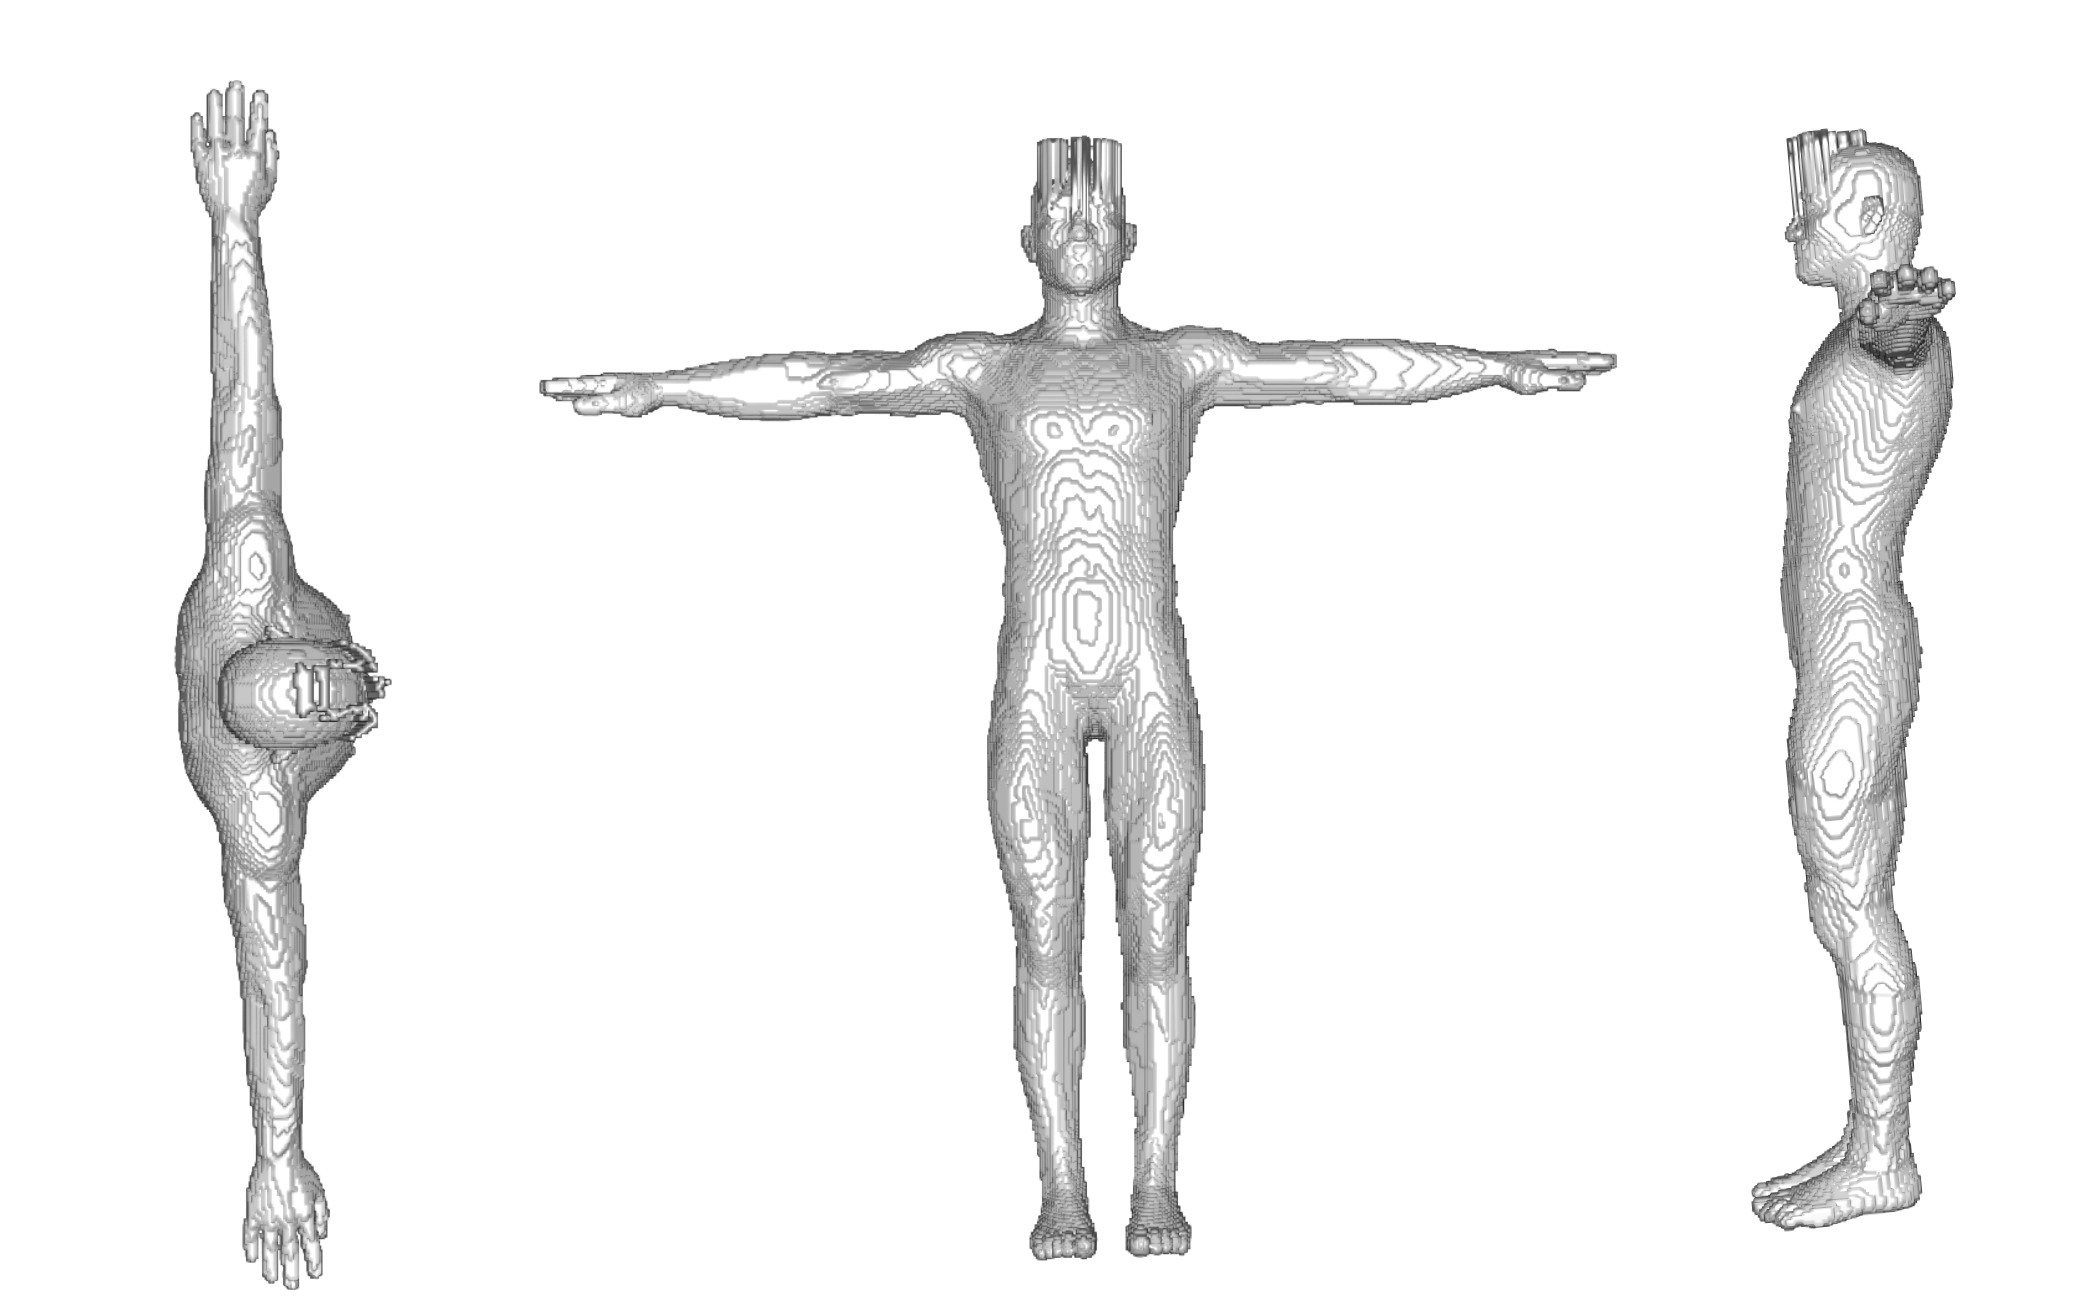
\includegraphics[width=11cm]{content/images/results/TPosition.png}
	\caption{The initial pose of the phantom data used to evaluate the method against the standardized position \cite{Squidifier2010DetailedMan}.}
	\label{fig:tPose}
\end{figure}

The first part of the result section is mainly about the performance of algorithm on the presented phantom of a man. The structure will be that first the initial pose and the armature in the data will be presented and afterwards the final T-pose of the data which is the output of the method applied. Then there is a section which handles the fetus data which is unfortunately also phantom data. The second major part of this chapter is about an influence analysis where results are presented which did not perform well and represent the effects of different influences in the given input data.

\newpage
\section{Performance of the algorithm}

\begin{figure} [htb!]
    \centering
	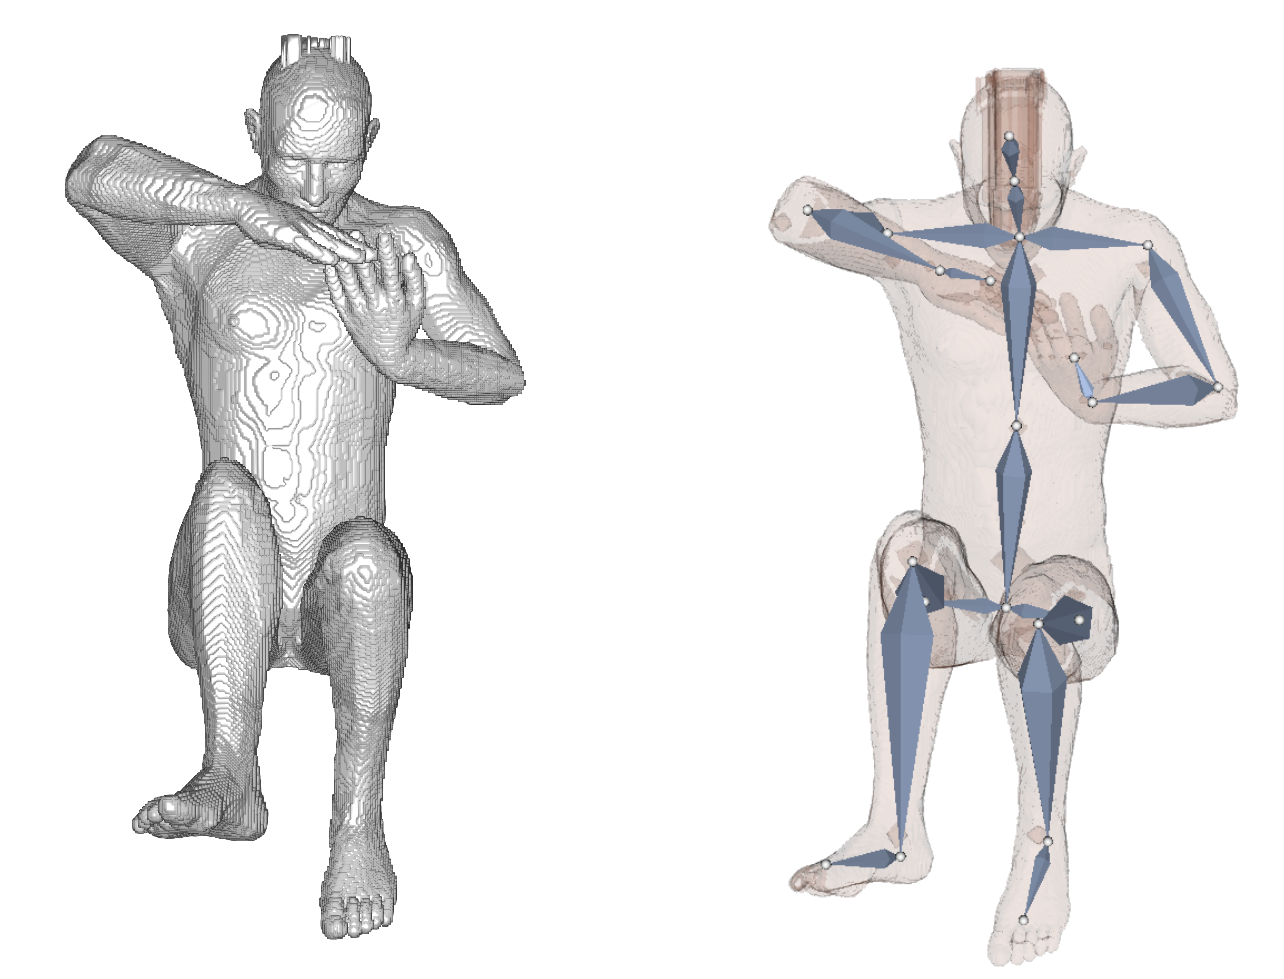
\includegraphics[width=13cm]{content/images/results/man1Front.png}
	\caption{Front view of the first fetus pose. On the left the volume visualization of the prototype and on the right the visualization of the included armature.}
	\label{fig:}
\end{figure}
\begin{figure} [htb!]
    \centering
	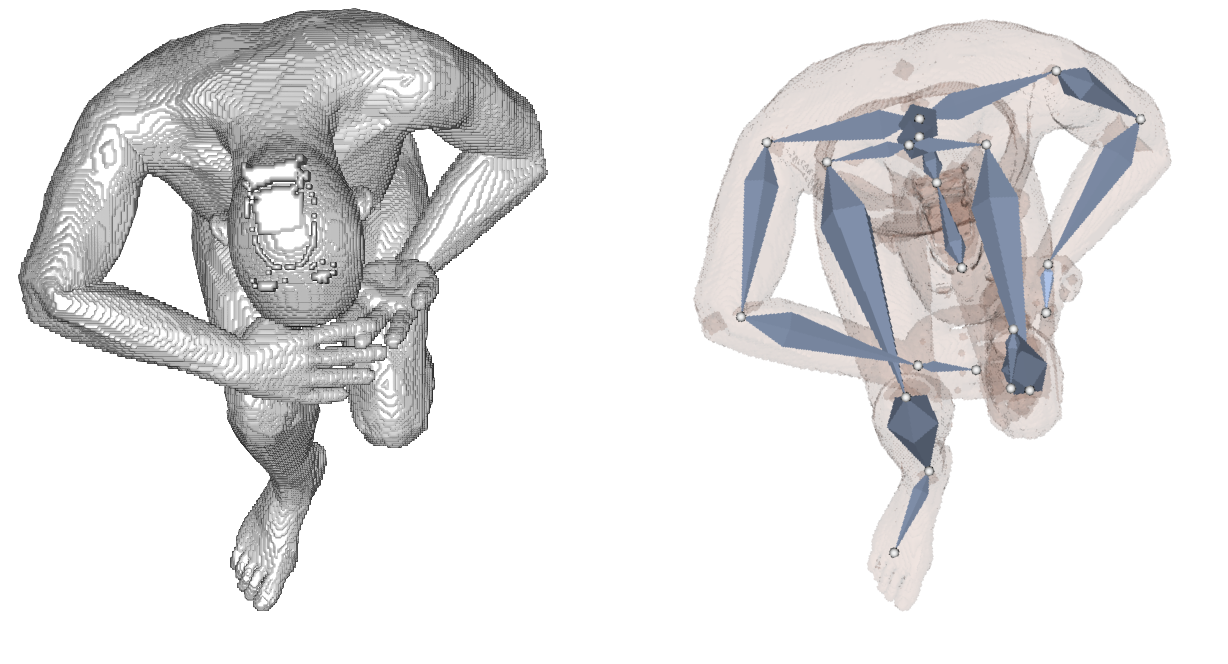
\includegraphics[width=13cm]{content/images/results/man1Top.png}
	\caption{Top view of the same formation also volume and armature view.}
	\label{fig:}
\end{figure}

\begin{figure} [htb!]
    \centering
	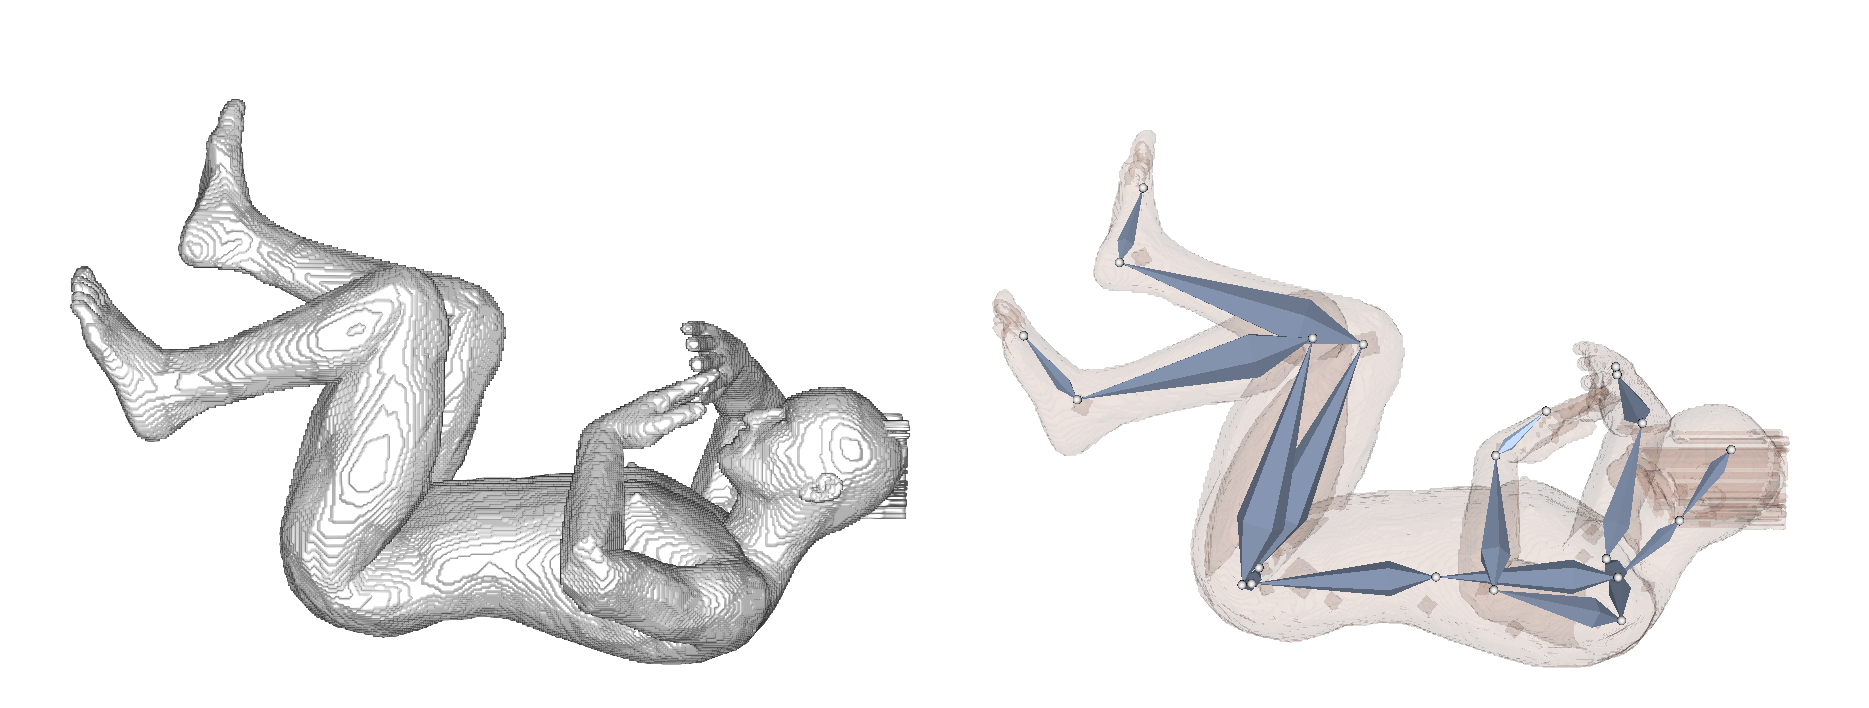
\includegraphics[width=15cm]{content/images/results/man1Side.png}
	\caption{Side view of the pose also with visible armature and volume visualization.}
	\label{fig:}
\end{figure}

\vspace*{2cm}

\begin{figure} [htb!]
    \centering
	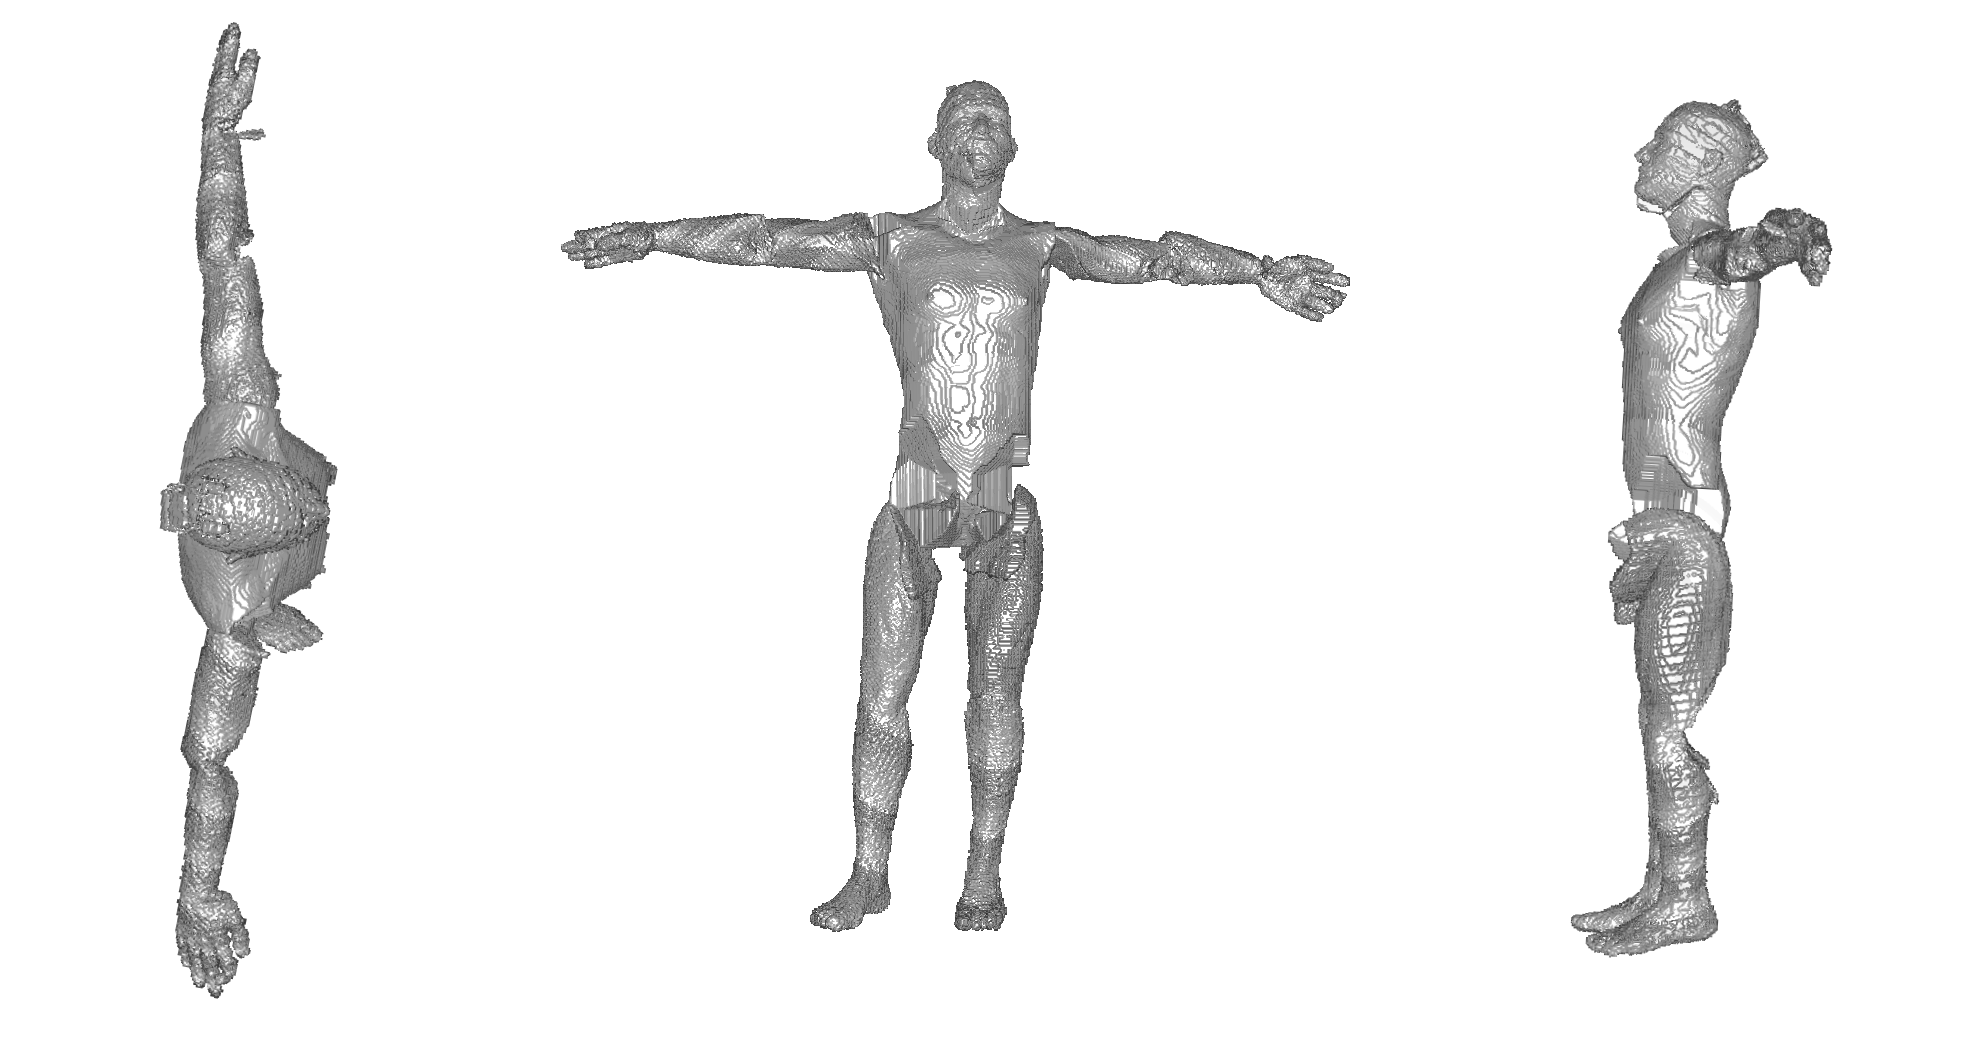
\includegraphics[width=16cm]{content/images/results/man1Result.png}
	\caption{The result T-pose of the first fetus pose from left to right: Top view, front view and side view.}
	\label{fig:}
\end{figure}
%% START MAN 2
\newpage
\begin{figure} [htb!]
    \centering
	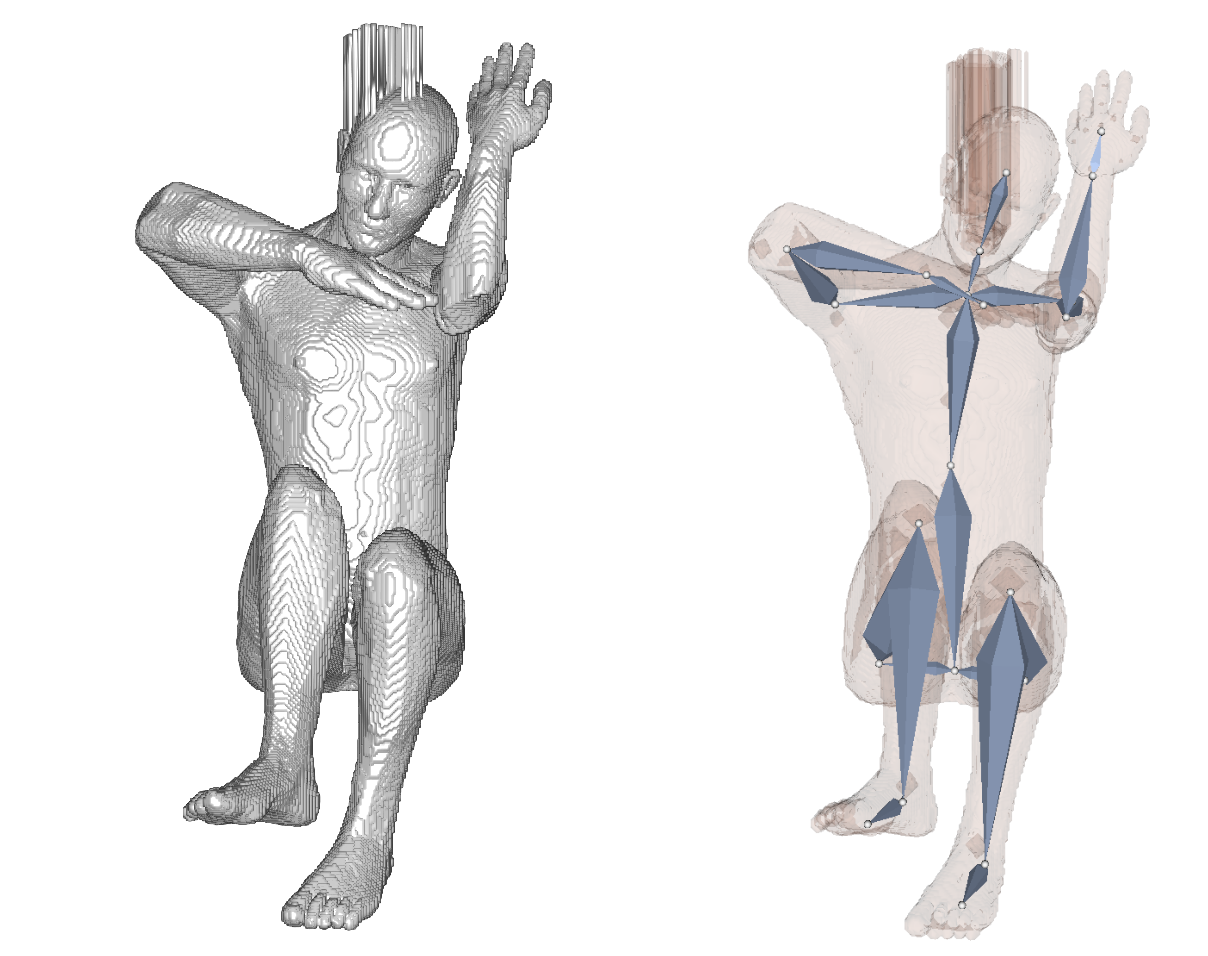
\includegraphics[width=13cm]{content/images/results/man2Front.png}
	\caption{Front view of the second fetus pose. On the left the volume visualization of the prototype and on the right the visualization of the included armature.}
	\label{fig:}
\end{figure}
\begin{figure} [htb!]
    \centering
	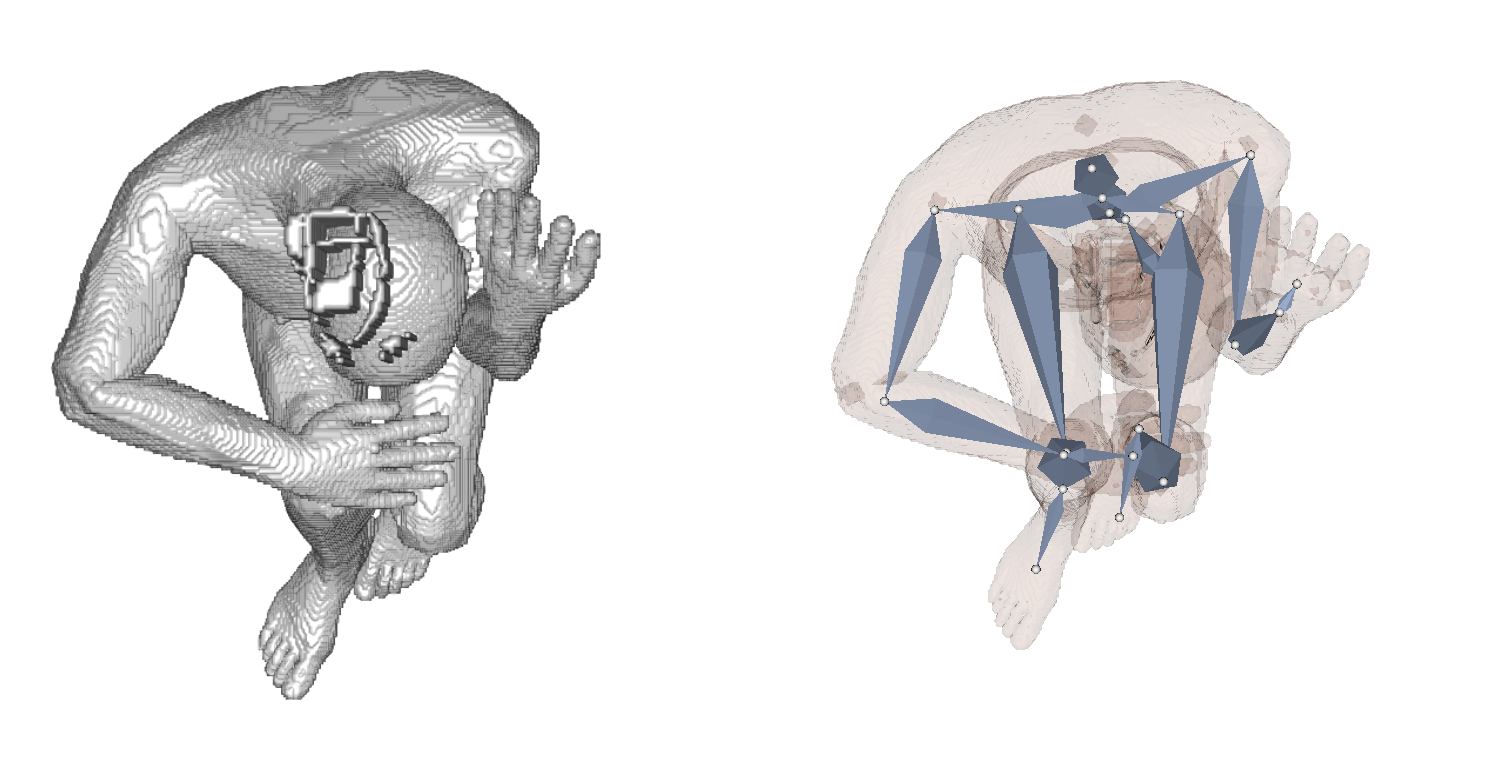
\includegraphics[width=13cm]{content/images/results/man2Top.png}
	\caption{Top view of the same formation also volume and armature view.}
	\label{fig:}
\end{figure}

\begin{figure} [htb!]
    \centering
	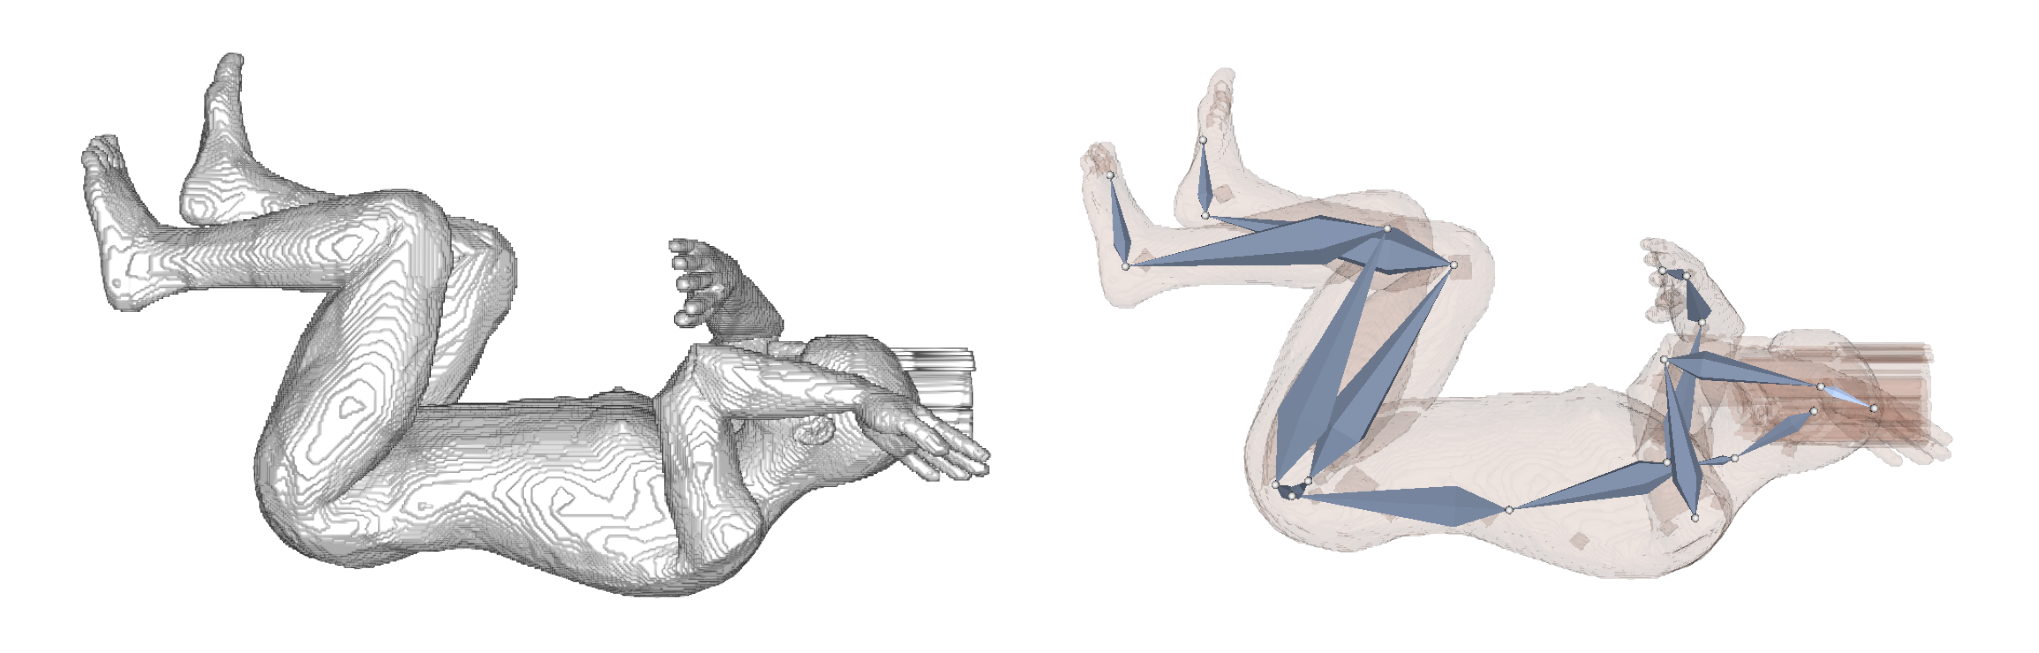
\includegraphics[width=15cm]{content/images/results/man2Side.png}
	\caption{Side view of the pose also with visible armature and volume visualization.}
	\label{fig:}
\end{figure}
\vspace*{3cm}
\begin{figure} [htb!]
    \centering
	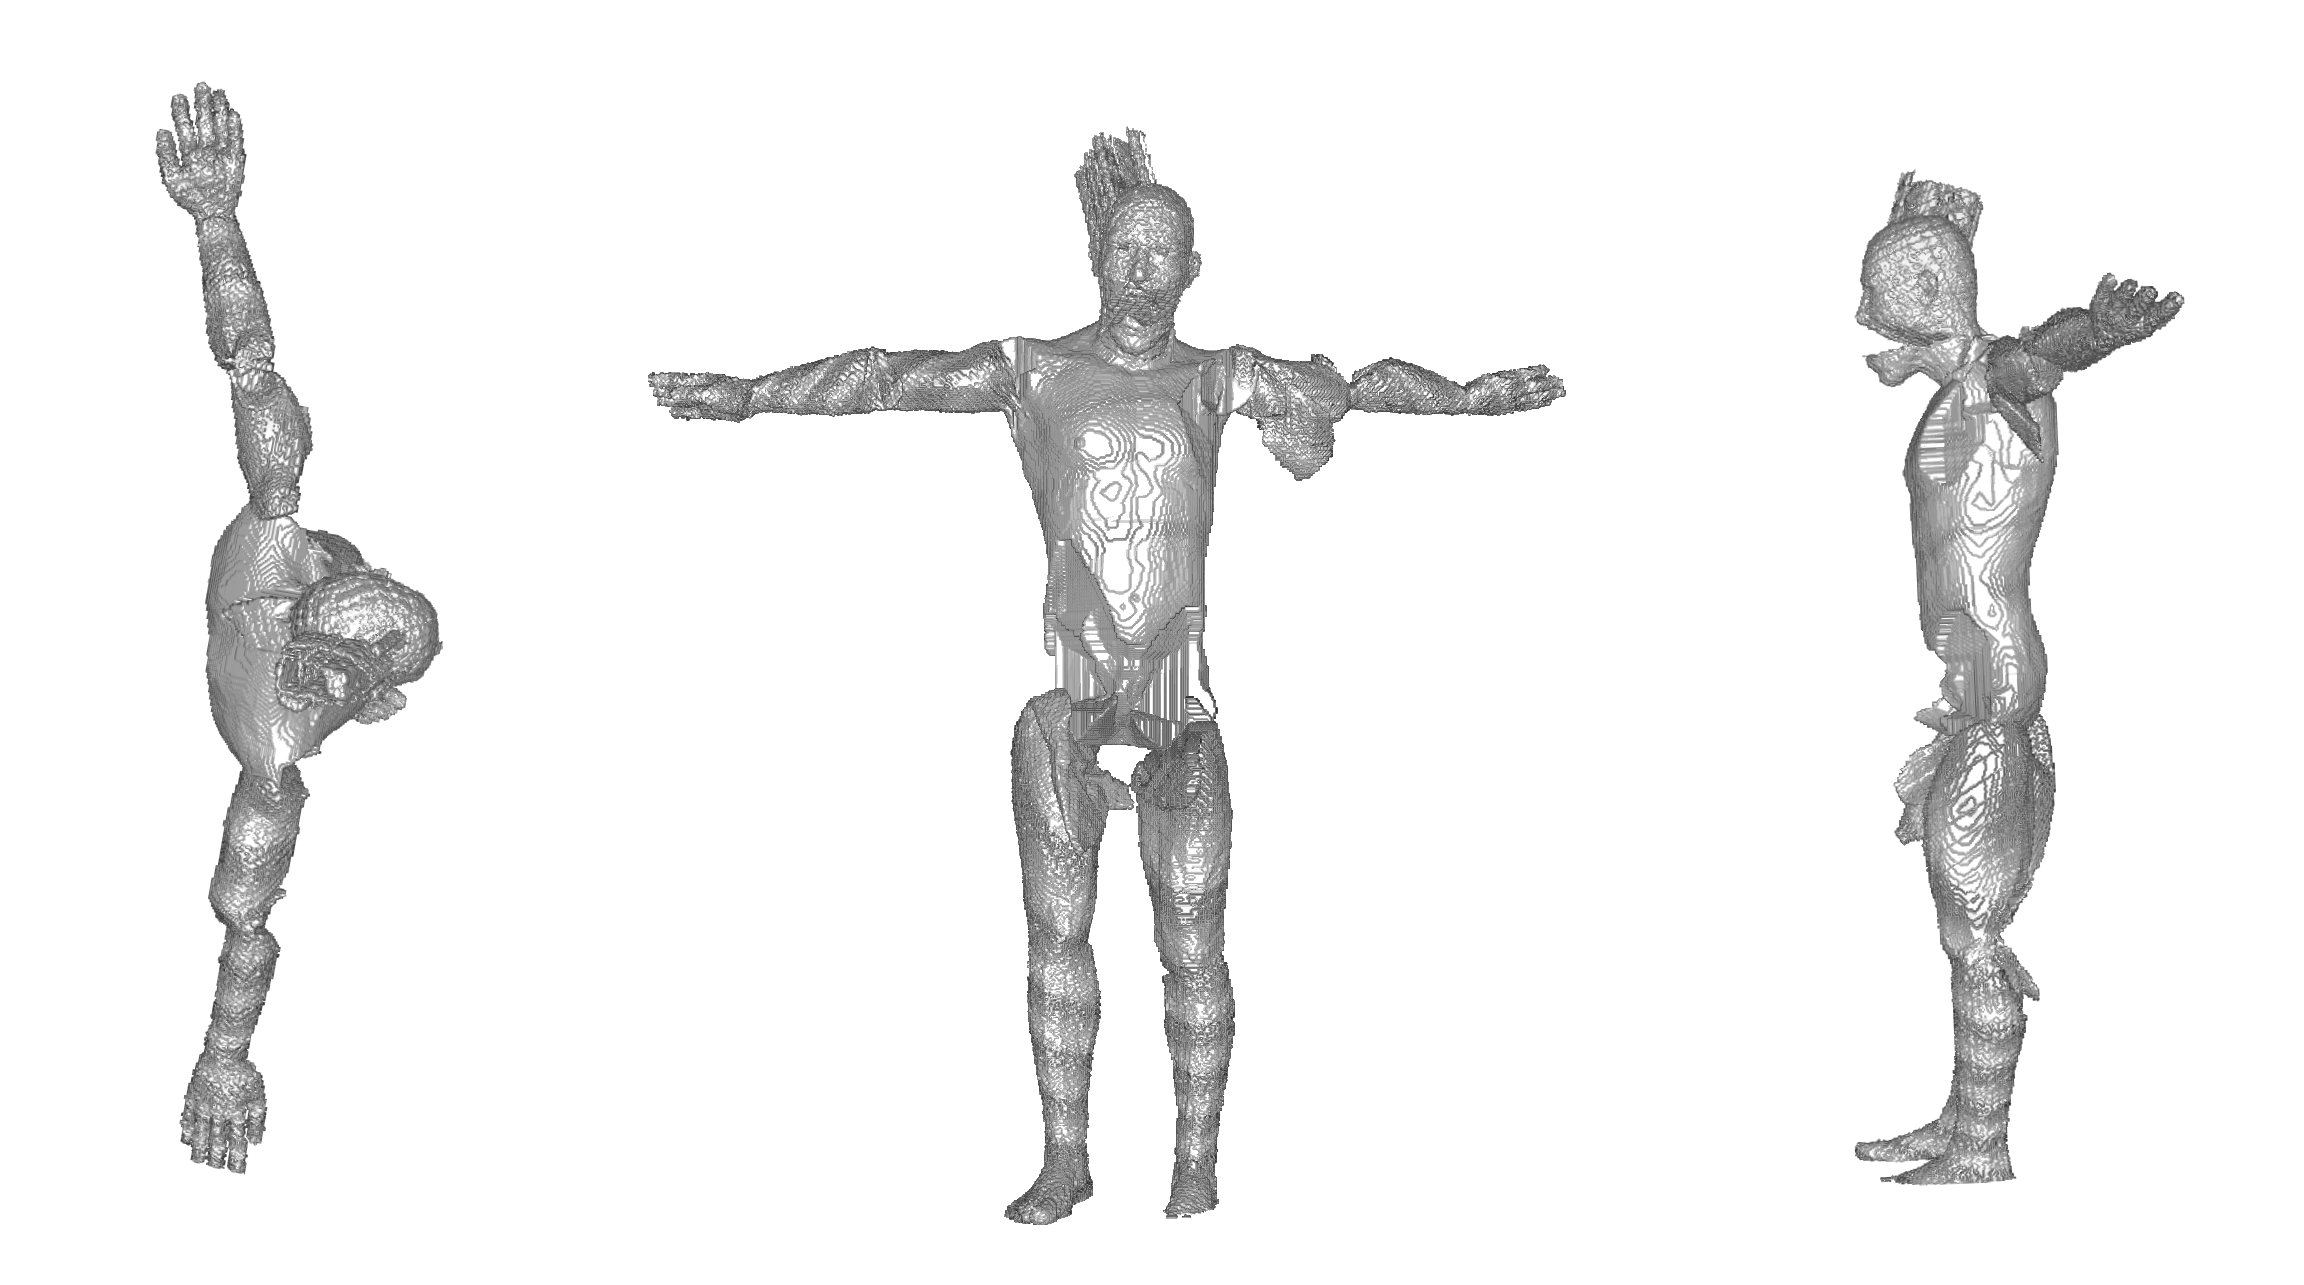
\includegraphics[width=15cm]{content/images/results/man2Result.png}
	\caption{The result T-pose of the second fetus pose from left to right: Top view, front view and side view.}
	\label{fig:}
\end{figure}
\newpage
%% START MEN 3
\begin{figure} [htb!]
    \centering
	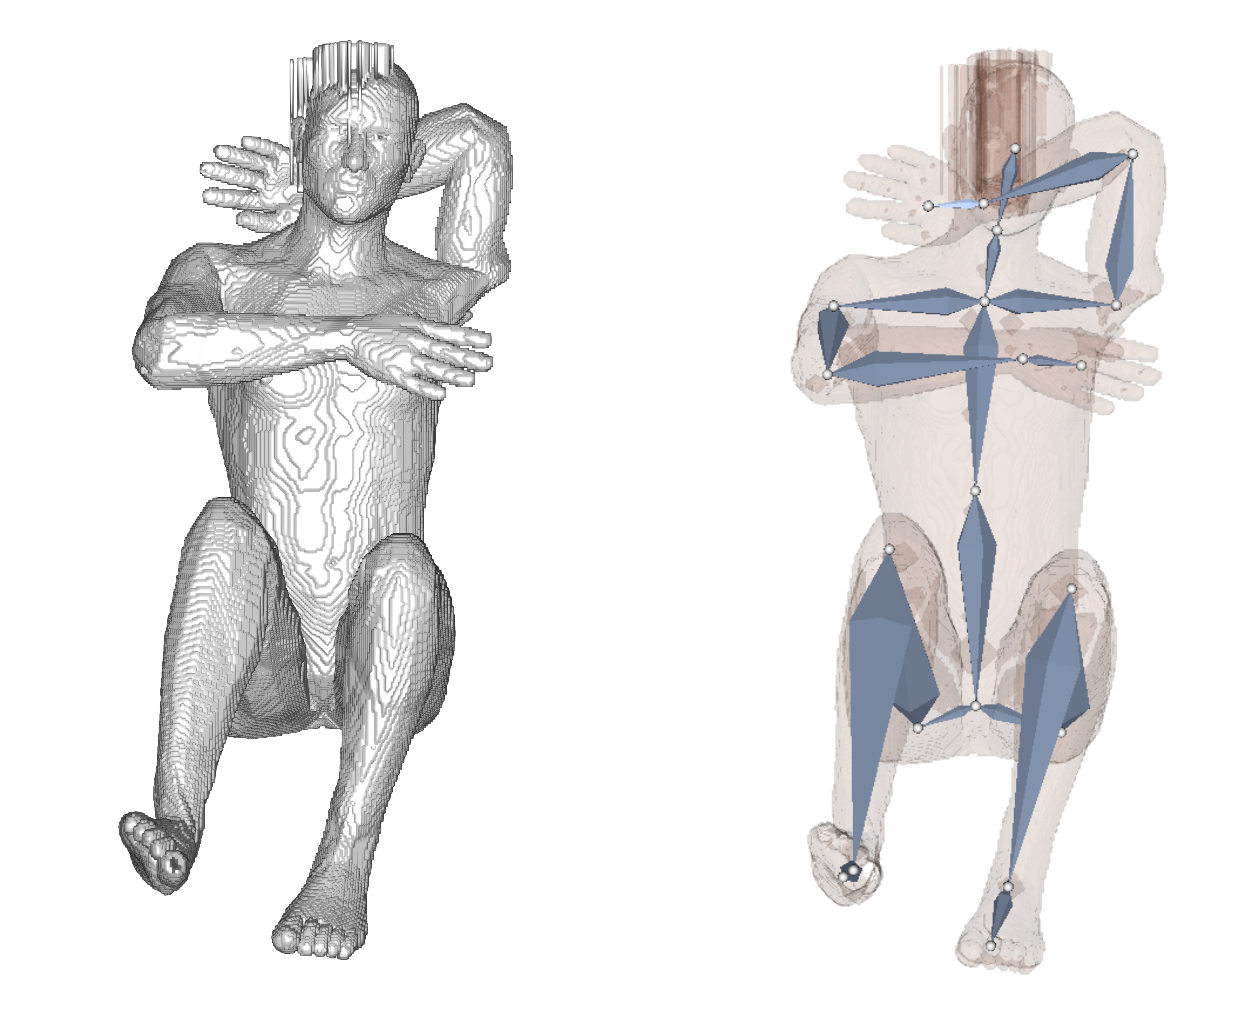
\includegraphics[width=13cm]{content/images/results/man3Front.png}
	\caption{Front view of the third fetus pose. On the left the volume visualization of the prototype and on the right the visualization of the included armature.}
	\label{fig:}
\end{figure}
\begin{figure} [htb!]
    \centering
	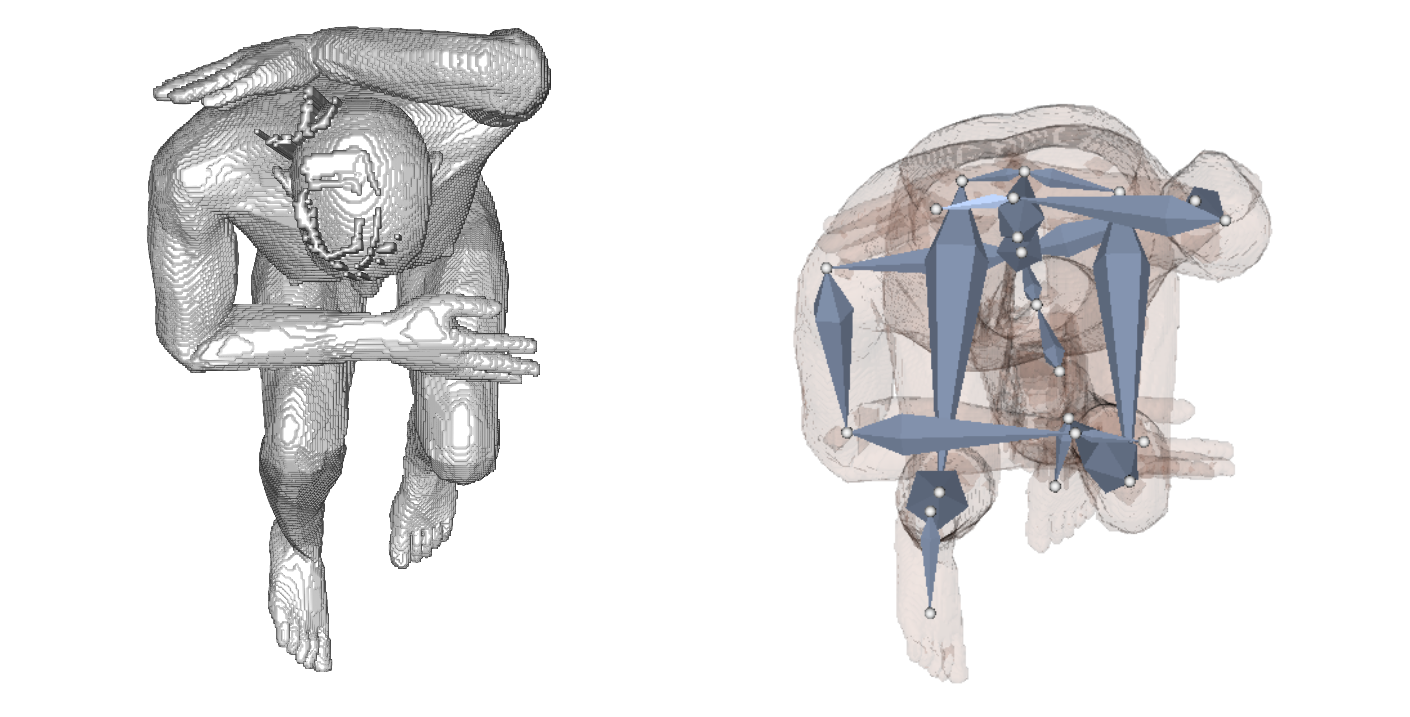
\includegraphics[width=13cm]{content/images/results/man3Top.png}
	\caption{Top view of the same formation also volume and armature view.}
	\label{fig:}
\end{figure}

\begin{figure} [htb!]
    \centering
	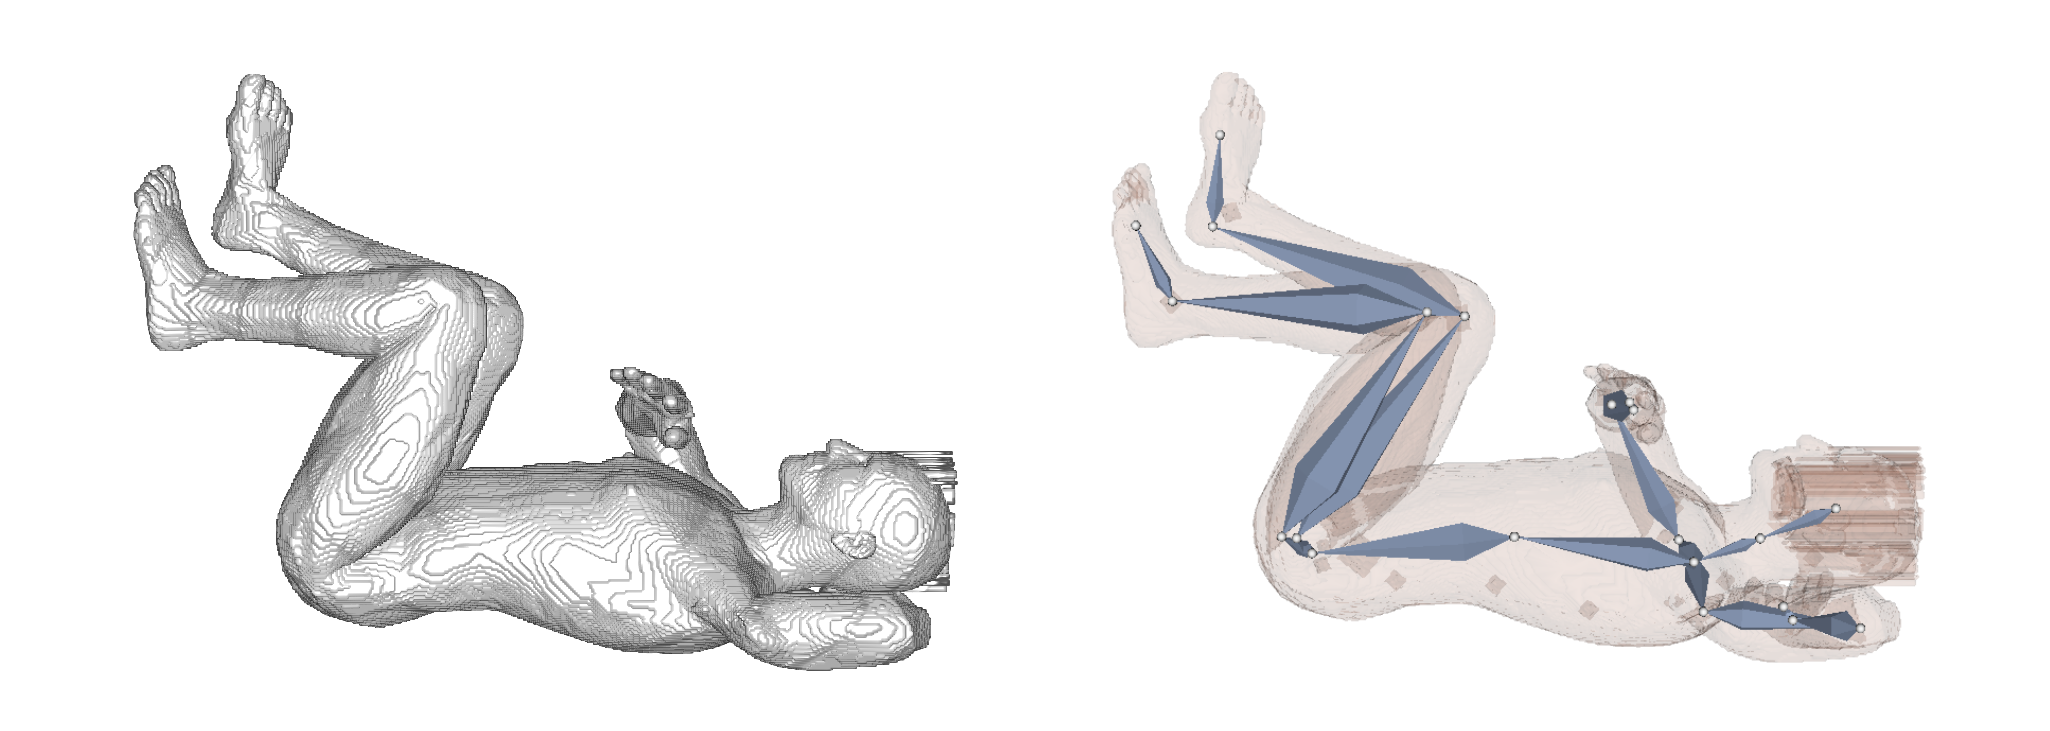
\includegraphics[width=15cm]{content/images/results/man3Side.png}
	\caption{Side view of the pose also with visible armature and volume visualization.}
	\label{fig:}
\end{figure}

\vspace{3cm}

\begin{figure} [htb!]
    \centering
	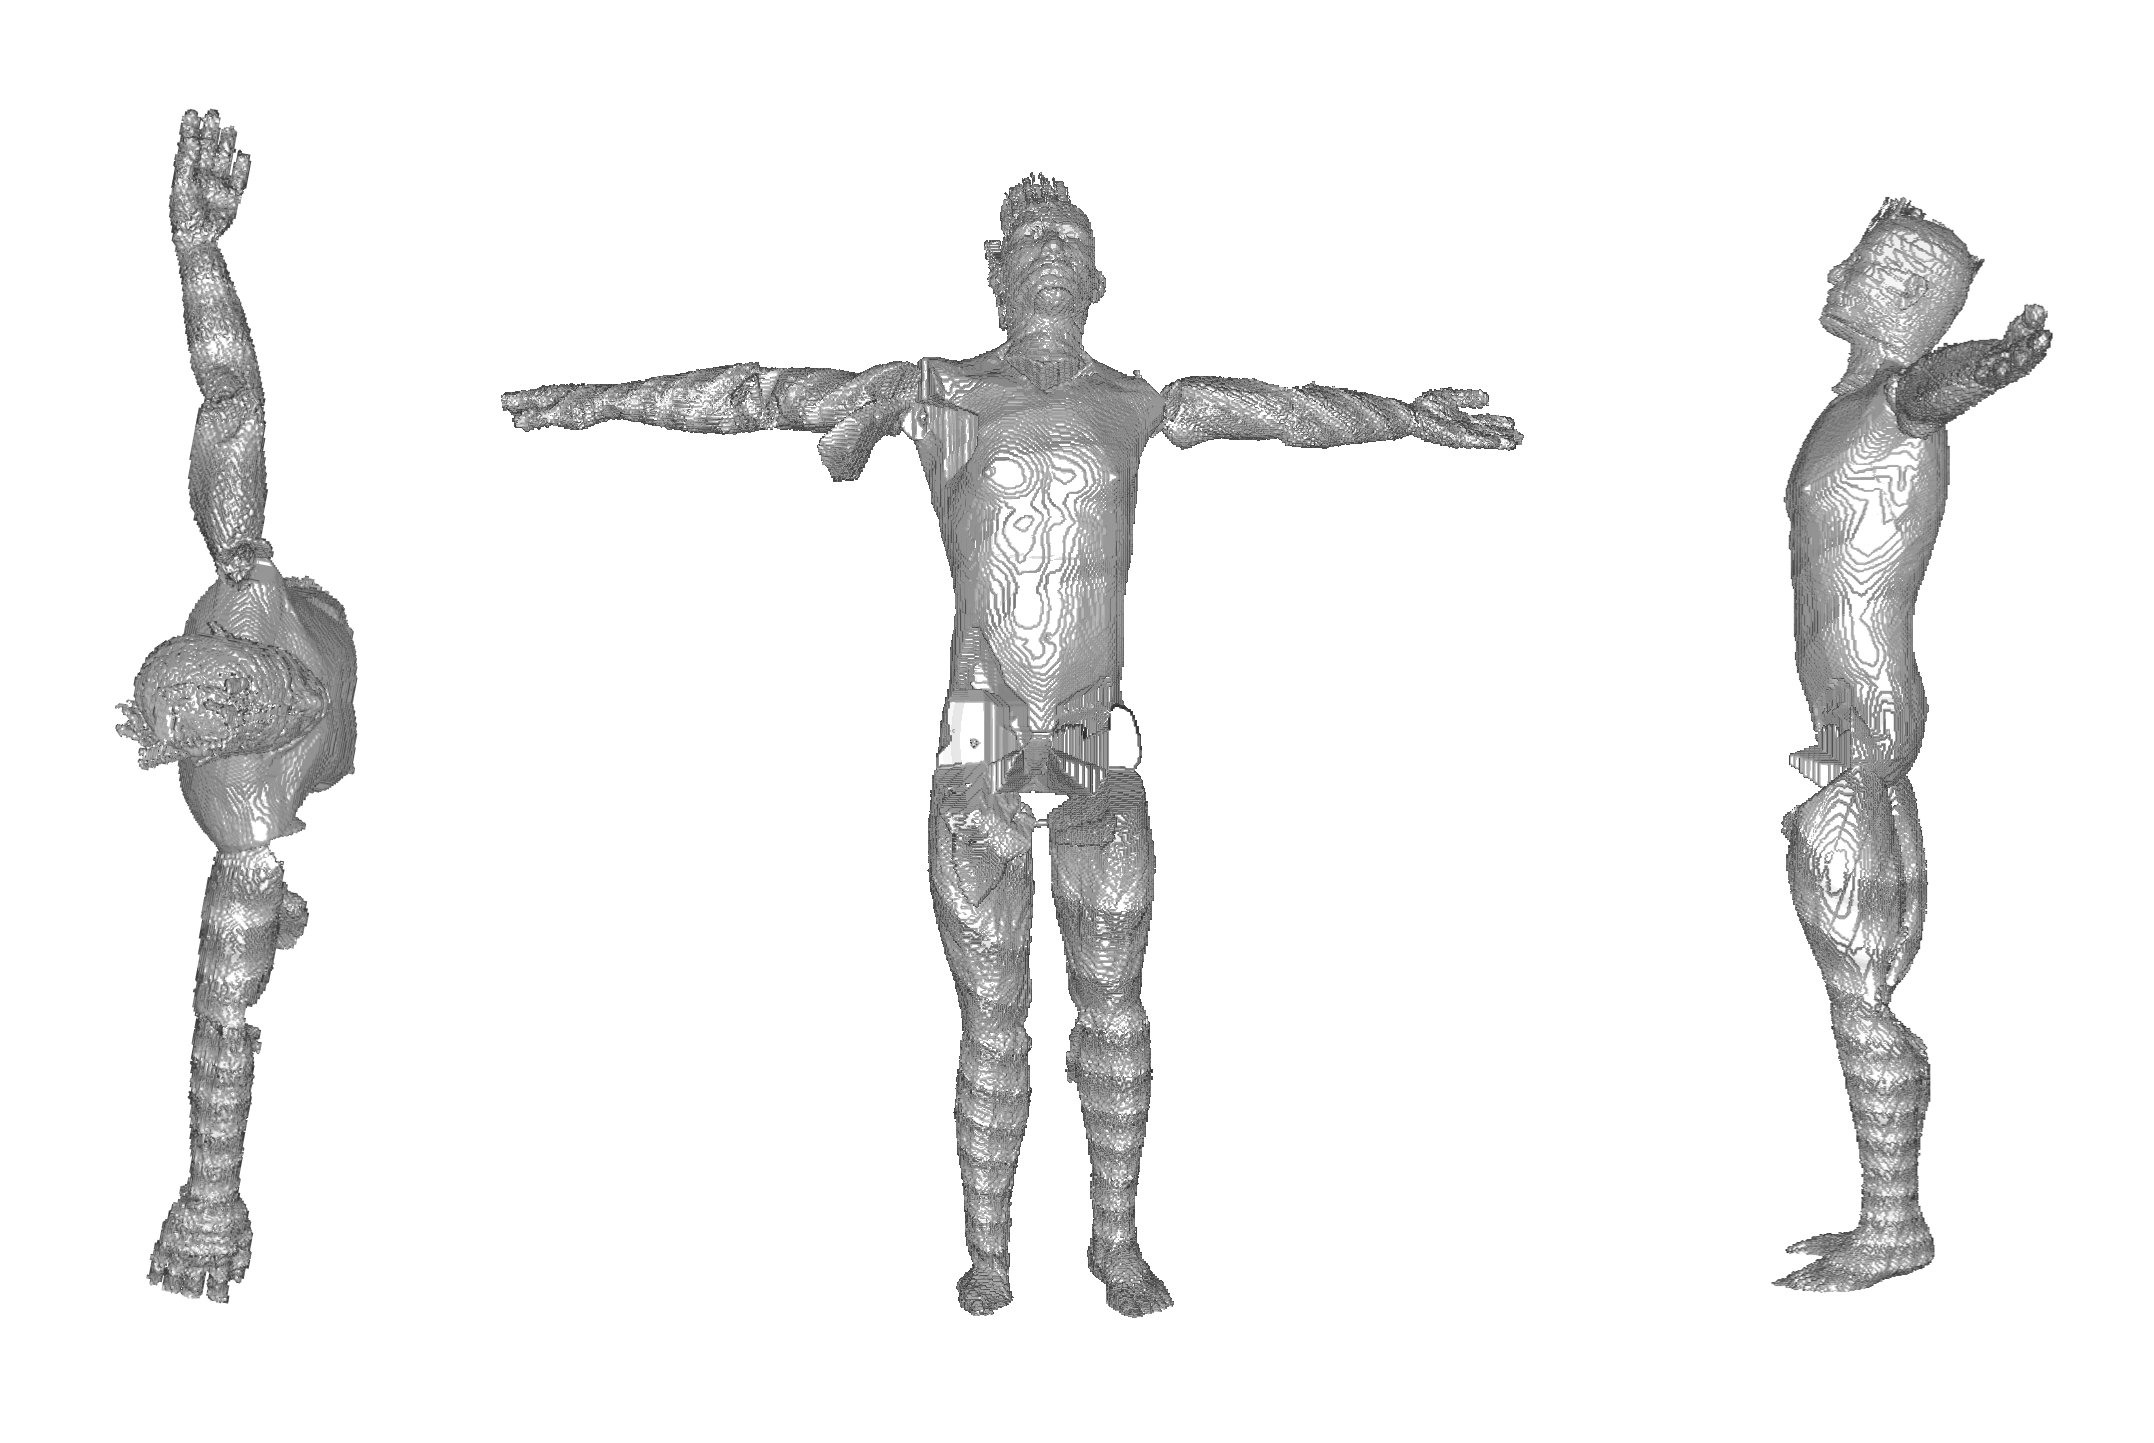
\includegraphics[width=15cm]{content/images/results/man3Result.png}
	\caption{The result T-pose of the third fetus pose from left to right: Top view, front view and side view.}
	\label{fig:}
\end{figure}
%% START MAN 4
\newpage
\begin{figure} [htb!]
    \centering
	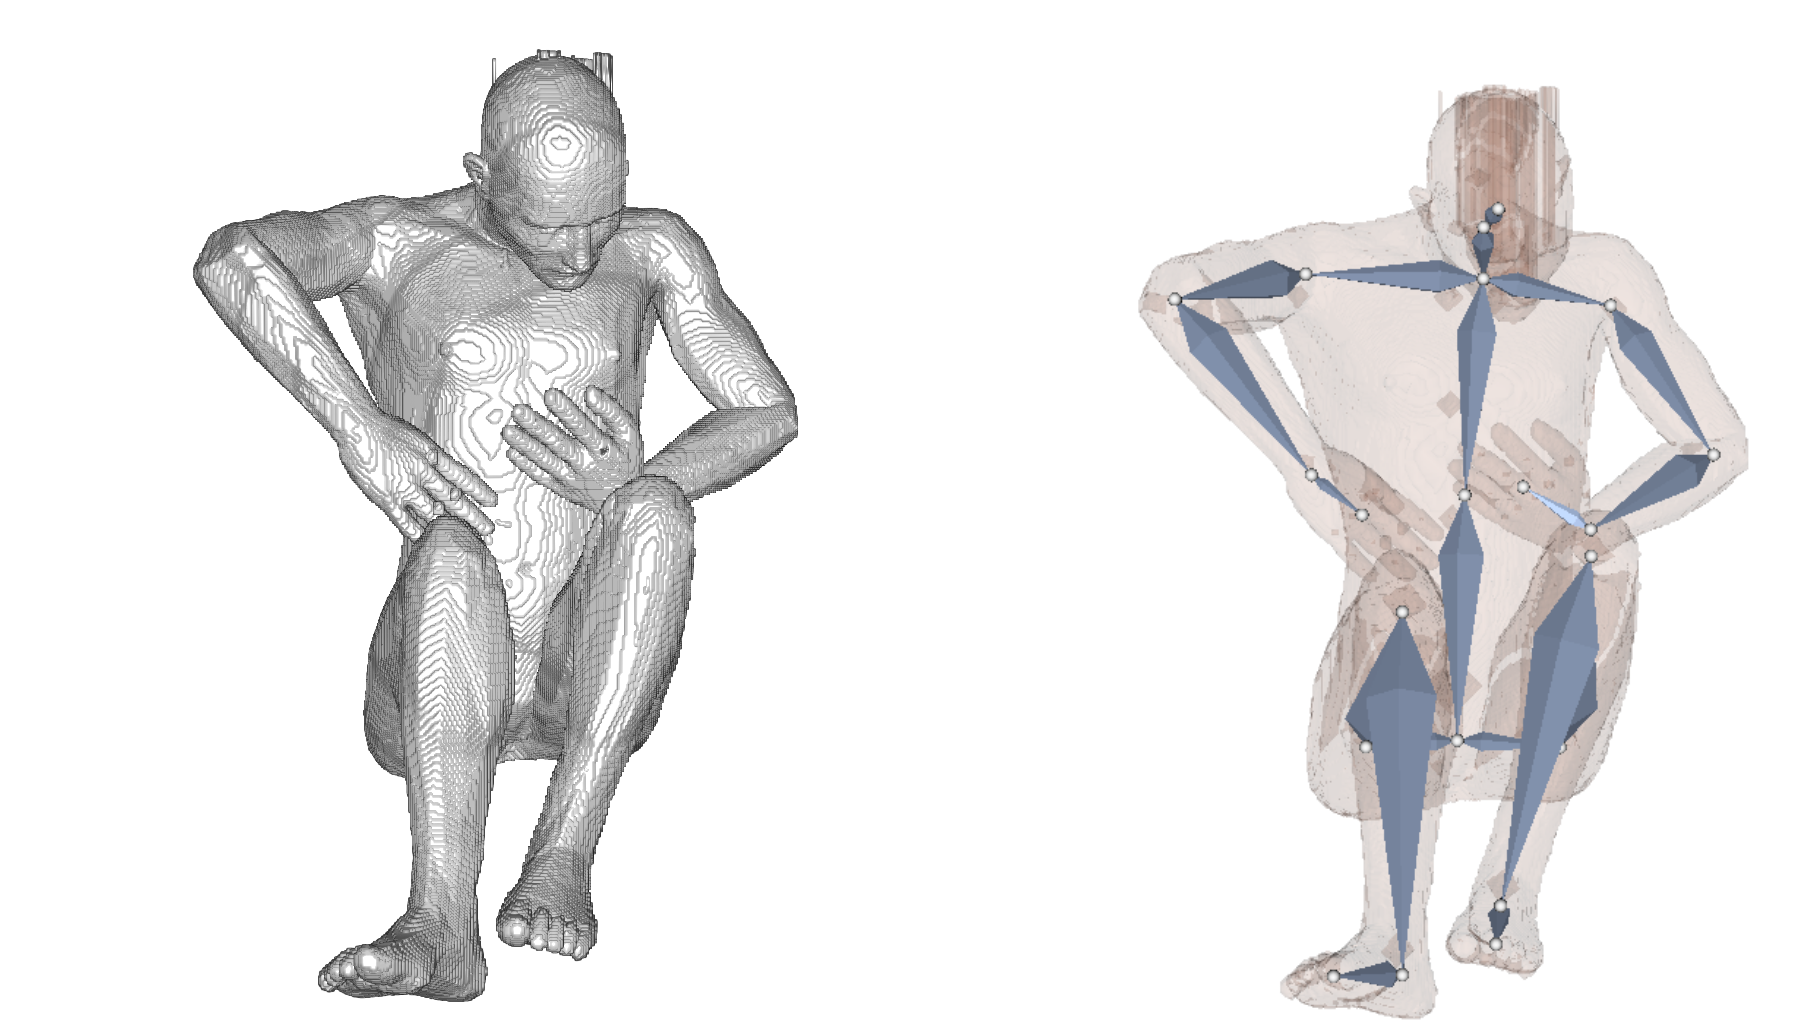
\includegraphics[width=13cm]{content/images/results/man4Front.png}
	\caption{Front view of the fourth fetus pose. On the left the volume visualization of the prototype and on the right the visualization of the included armature.}
	\label{fig:}
\end{figure}
\begin{figure} [htb!]
    \centering
	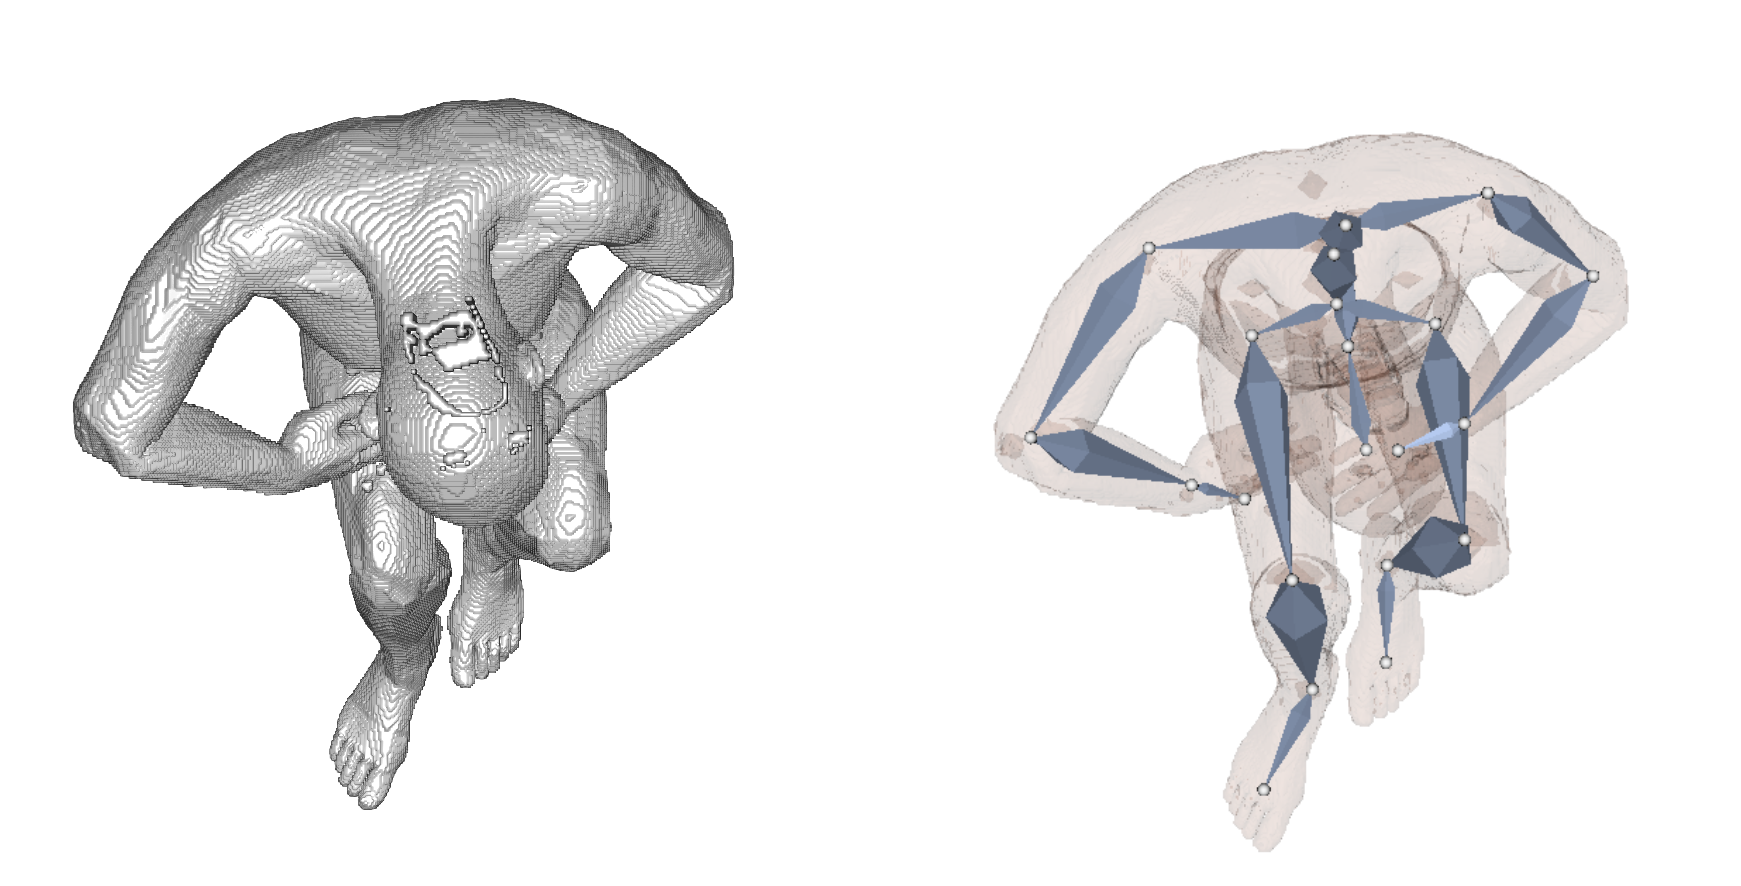
\includegraphics[width=13cm]{content/images/results/man4Top.png}
	\caption{Top view of the same formation also volume and armature view.}
	\label{fig:}
\end{figure}

\begin{figure} [htb!]
    \centering
	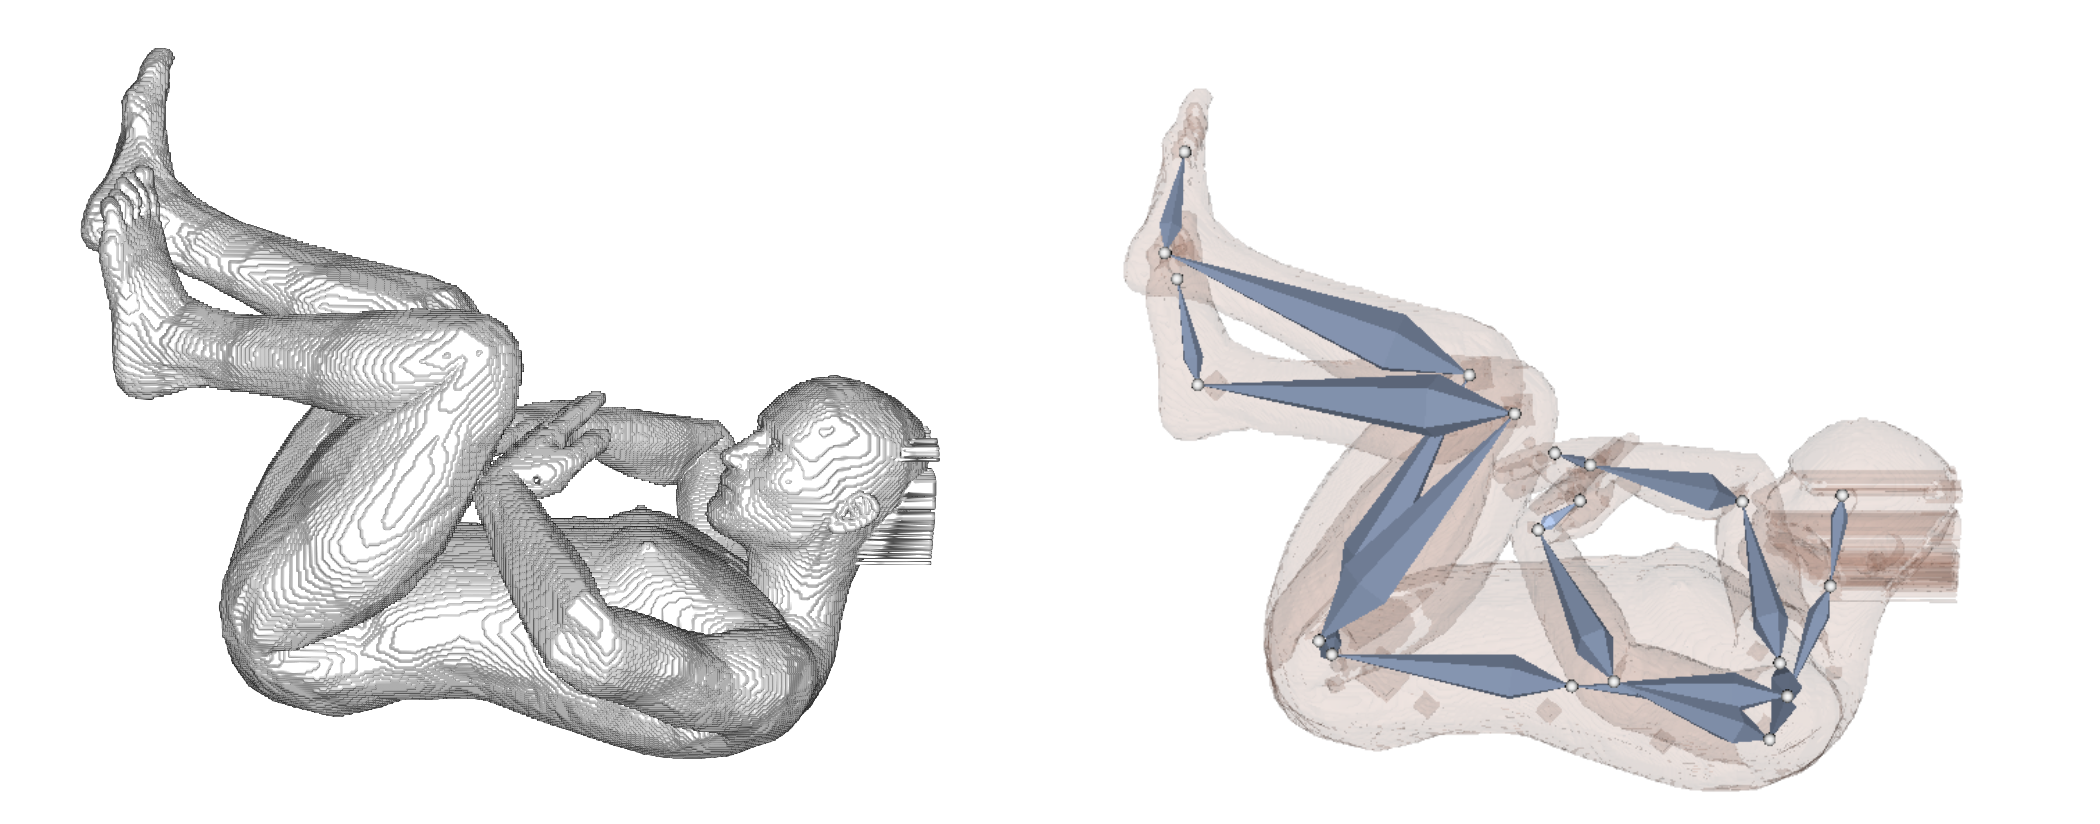
\includegraphics[width=15cm]{content/images/results/man4Side.png}
	\caption{Side view of the pose also with visible armature and volume visualization.}
	\label{fig:}
\end{figure}
\vspace*{3cm}
\begin{figure} [htb!]
    \centering
	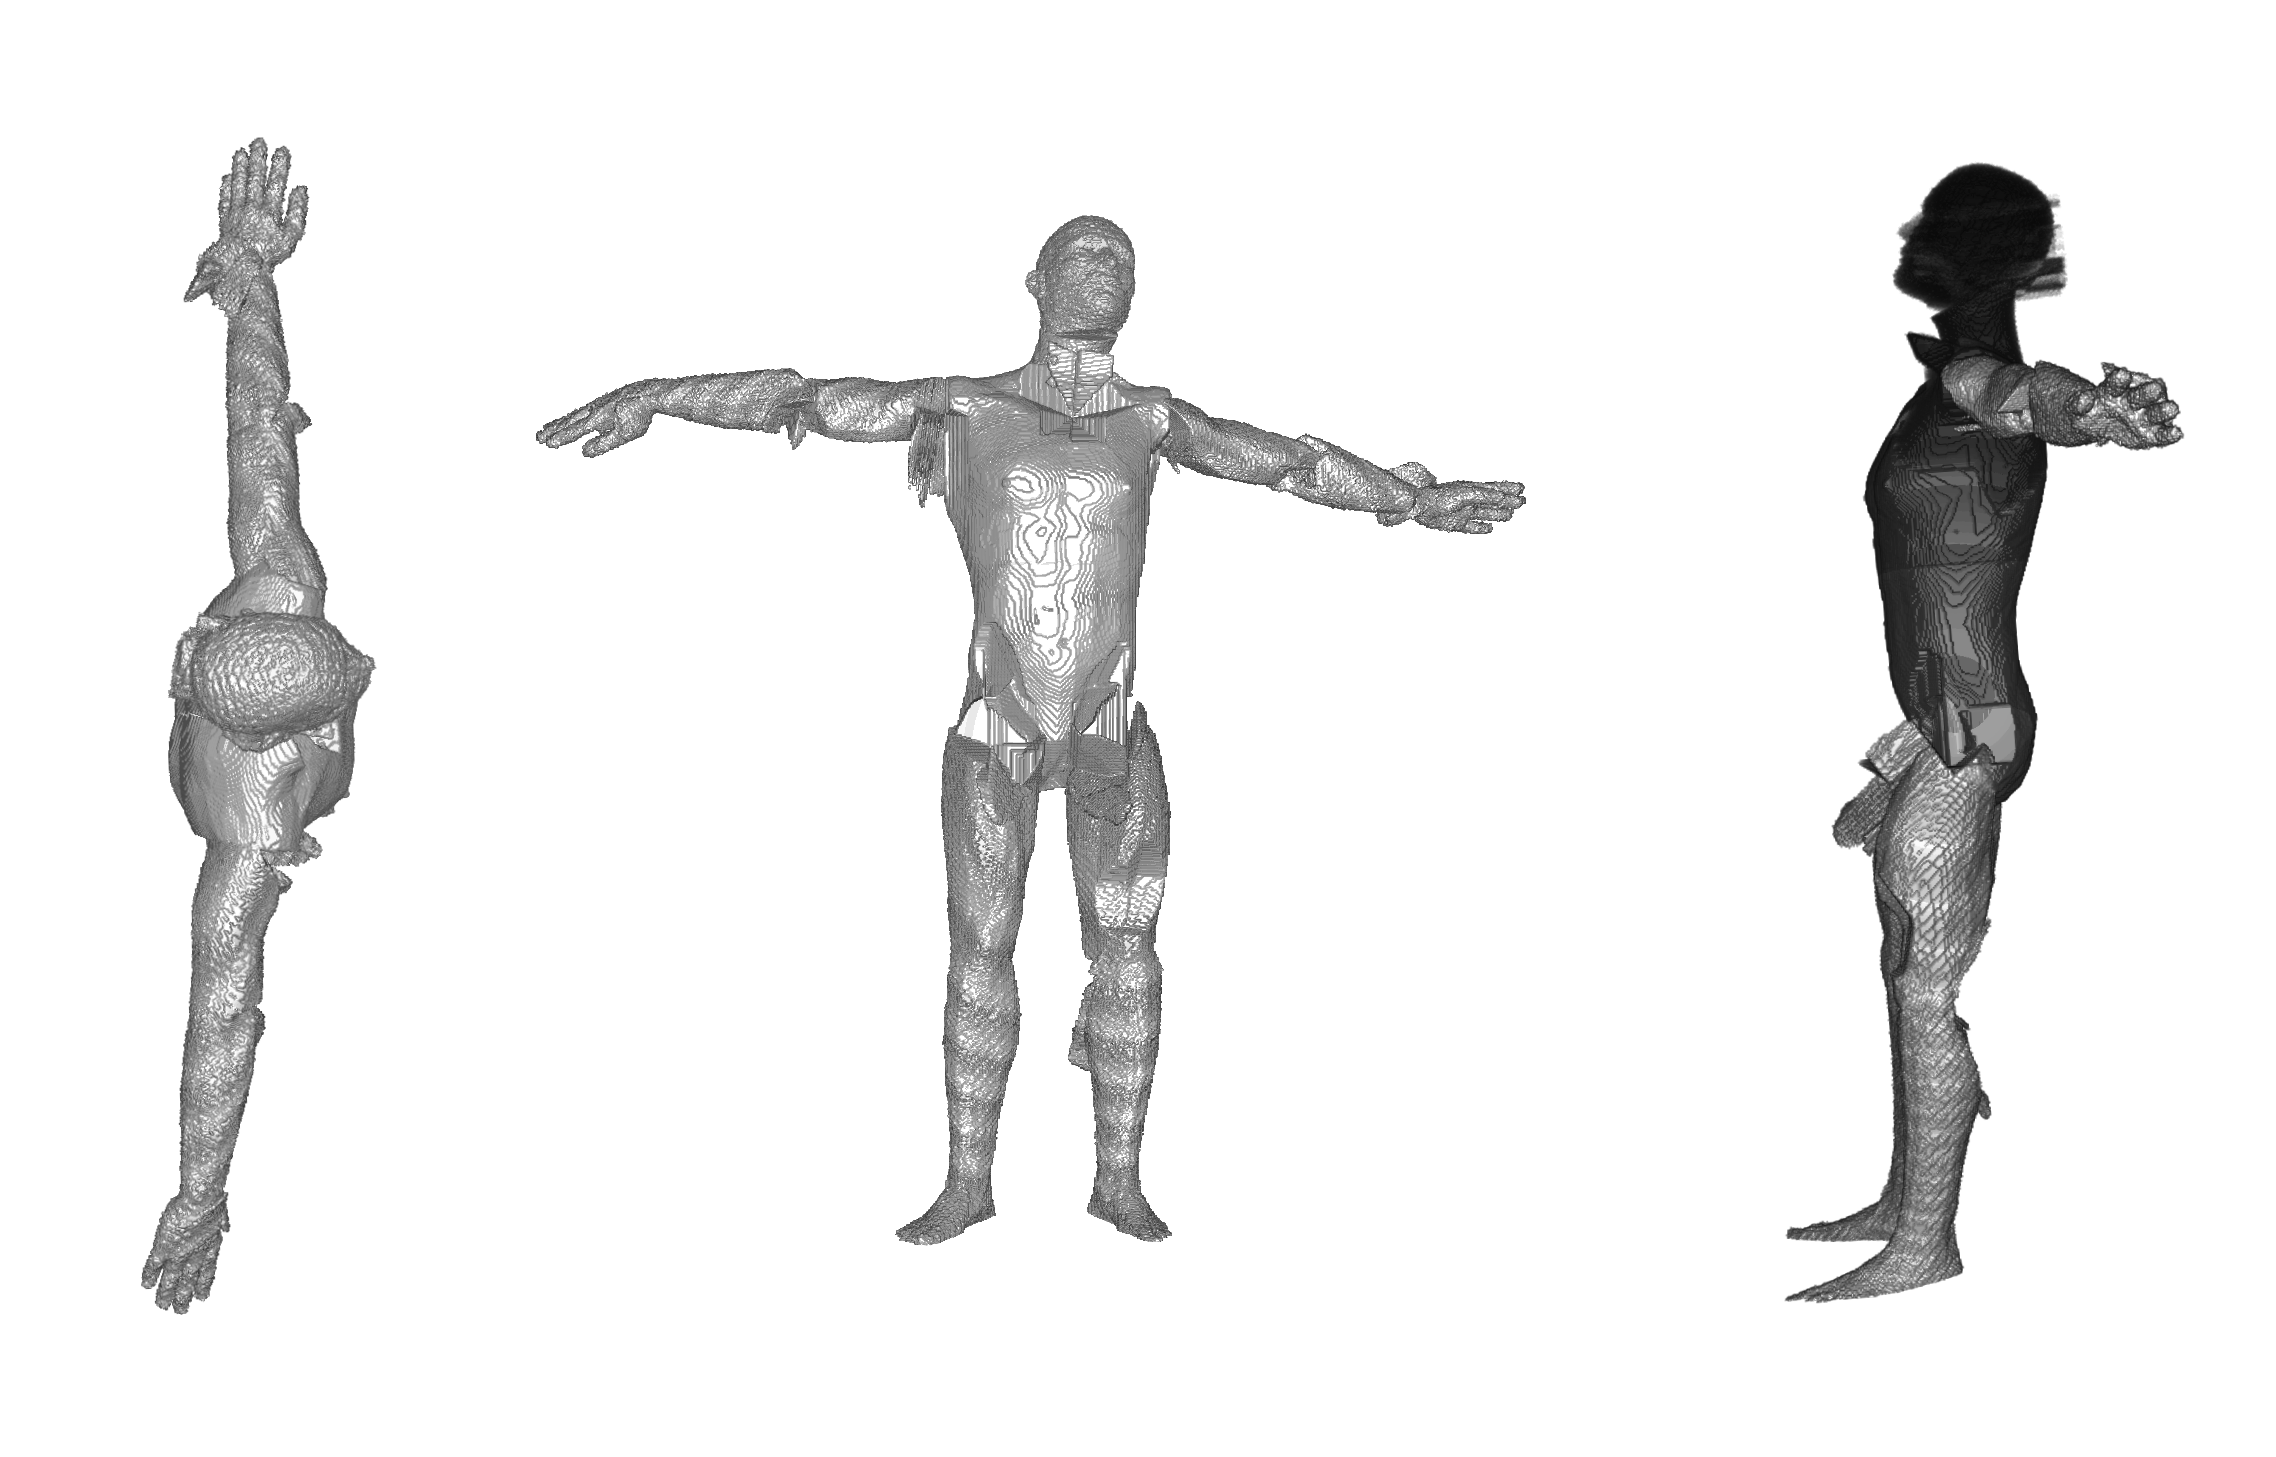
\includegraphics[width=16cm]{content/images/results/man4Result.png}
	\caption{The result T-pose of the fourth fetus pose from left to right: Top view, front view and side view.}
	\label{fig:}
\end{figure}
%% START MAN 5
\newpage
\begin{figure} [htb!]
    \centering
	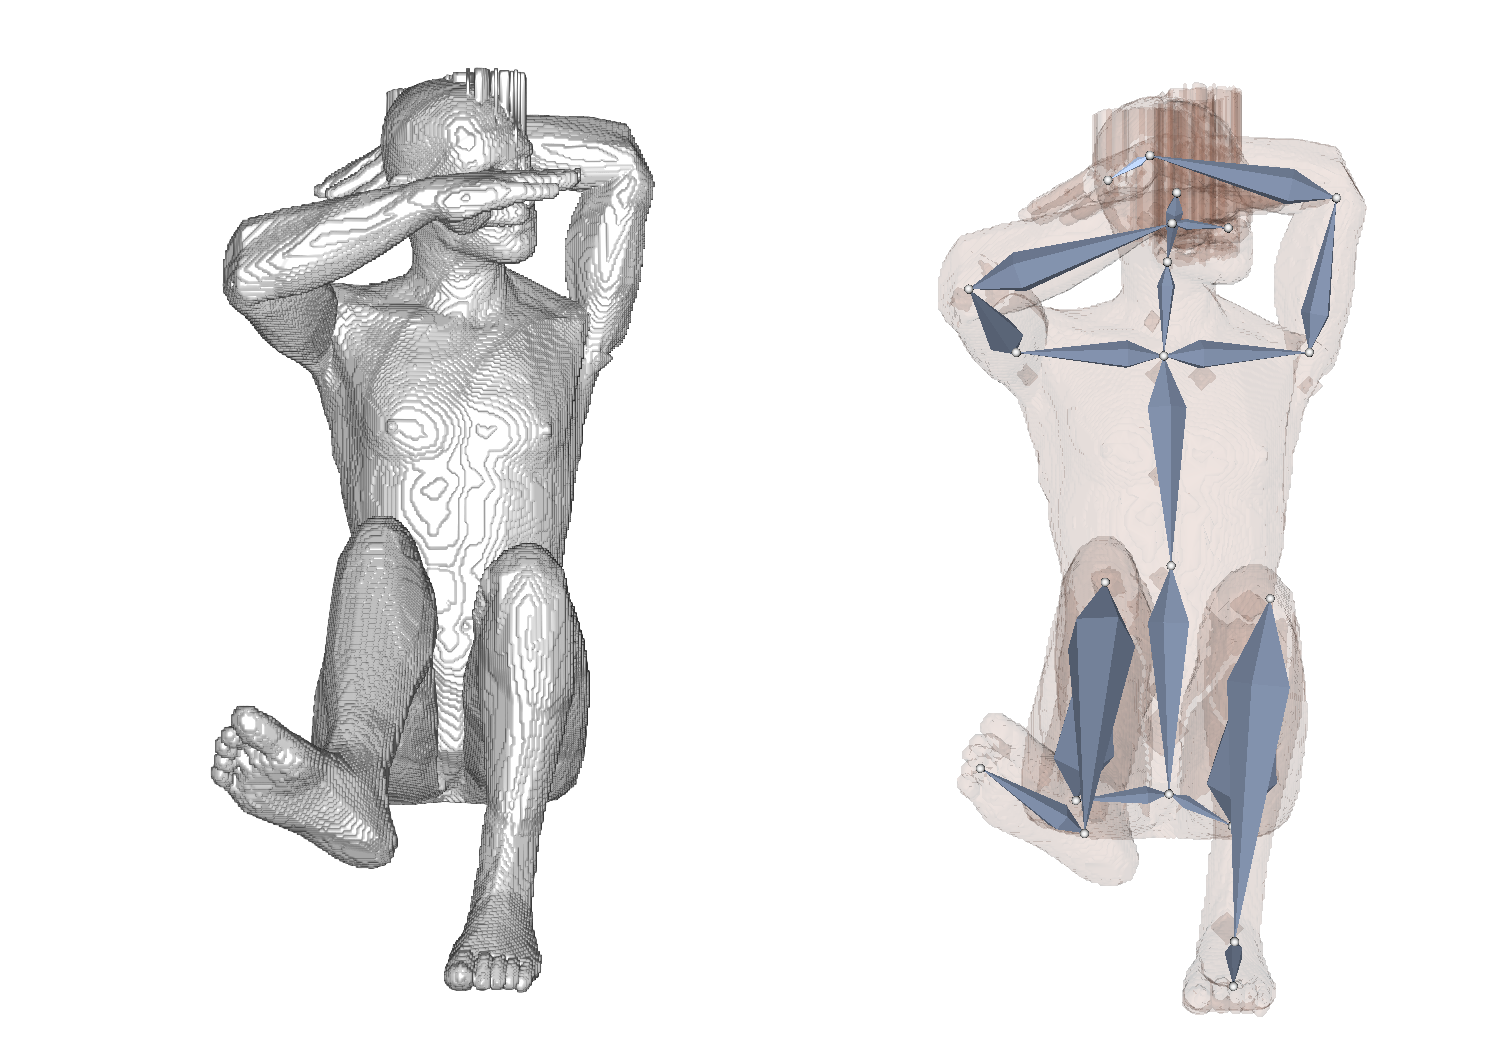
\includegraphics[width=13cm]{content/images/results/man5Front.png}
	\caption{Front view of the fifth fetus pose. On the left the volume visualization of the prototype and on the right the visualization of the included armature.}
	\label{fig:}
\end{figure}
\begin{figure} [htb!]
    \centering
	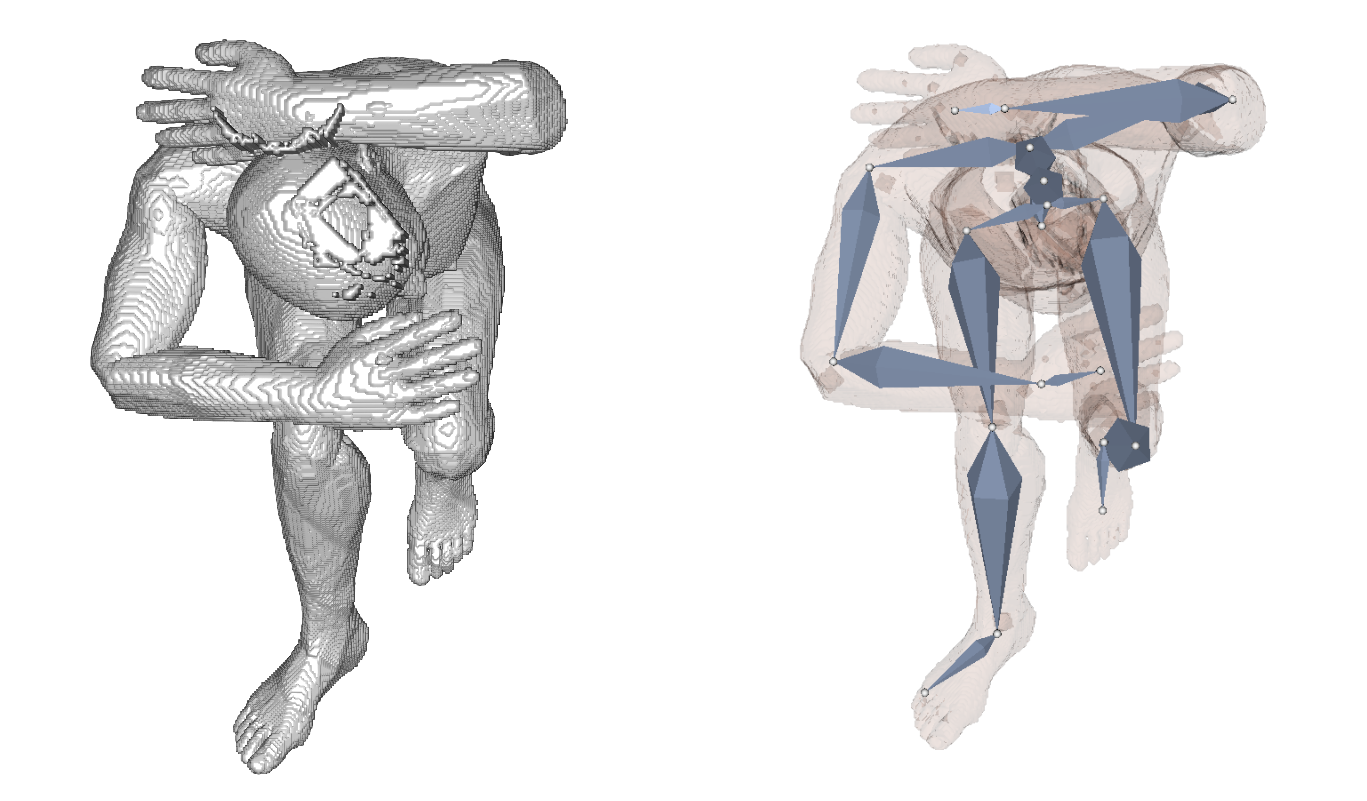
\includegraphics[width=13cm]{content/images/results/man5Top.png}
	\caption{Top view of the same formation also volume and armature view.}
	\label{fig:}
\end{figure}

\begin{figure} [htb!]
    \centering
	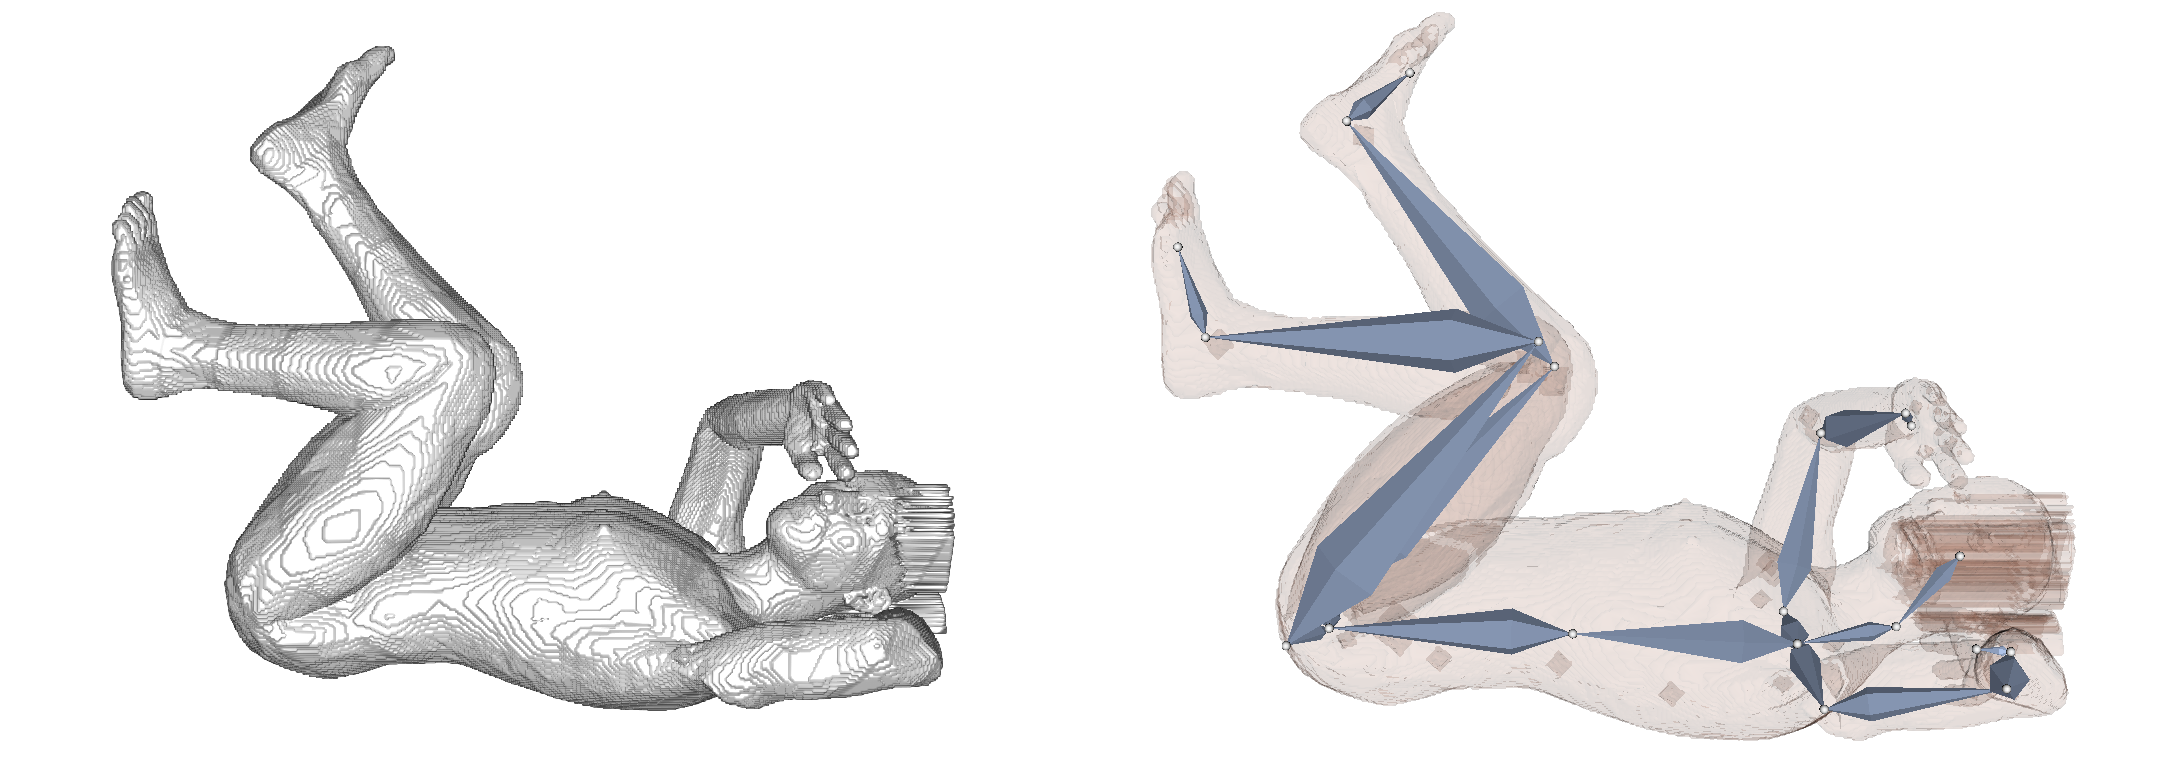
\includegraphics[width=15cm]{content/images/results/man5Side.png}
	\caption{Side view of the pose also with visible armature and volume visualization.}
	\label{fig:}
\end{figure}
\vspace{3cm}
\begin{figure} [htb!]
    \centering
	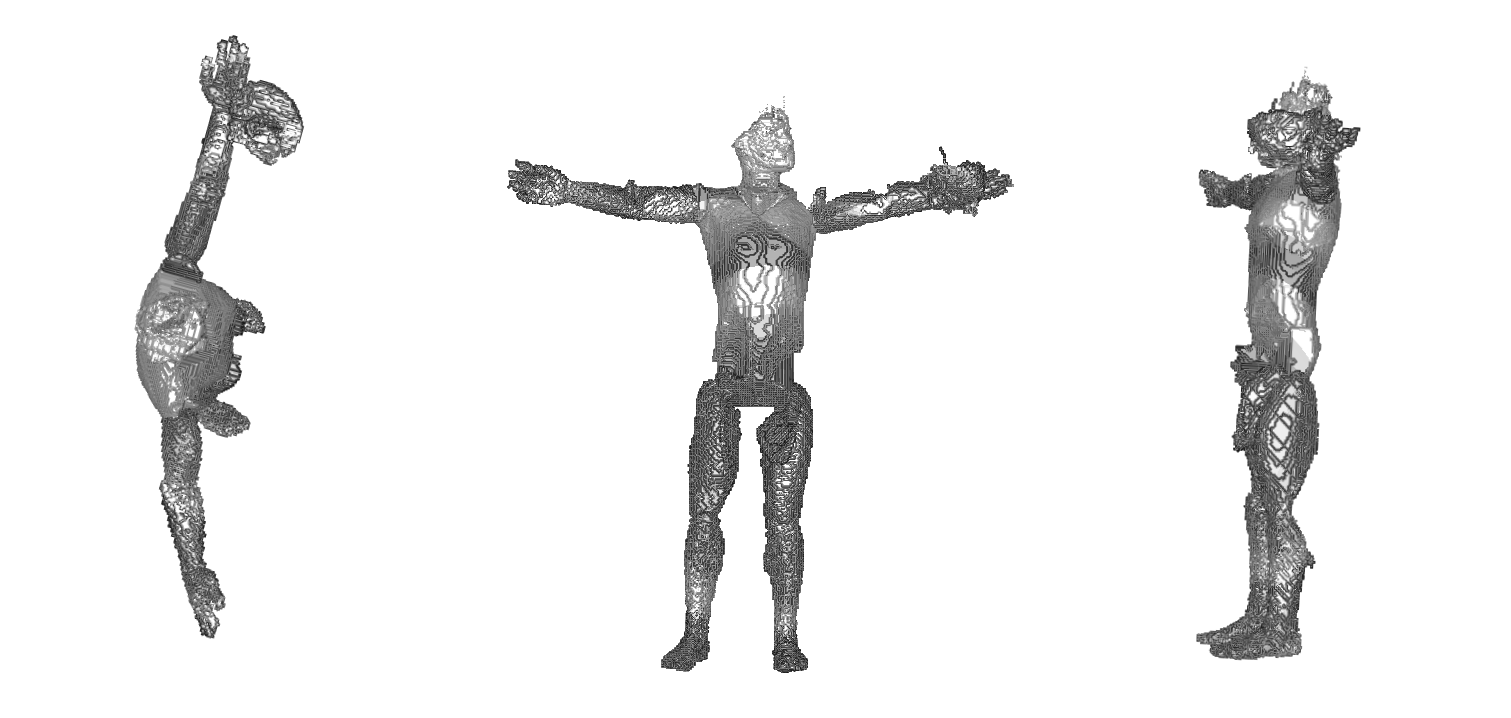
\includegraphics[width=16cm]{content/images/results/man5Result.png}
	\caption{The result T-pose of the fifth fetus pose from left to right: Top view, front view and side view.}
	\label{fig:}
\end{figure}

%% START MAN 6
\newpage
\begin{figure} [htb!]
    \centering
	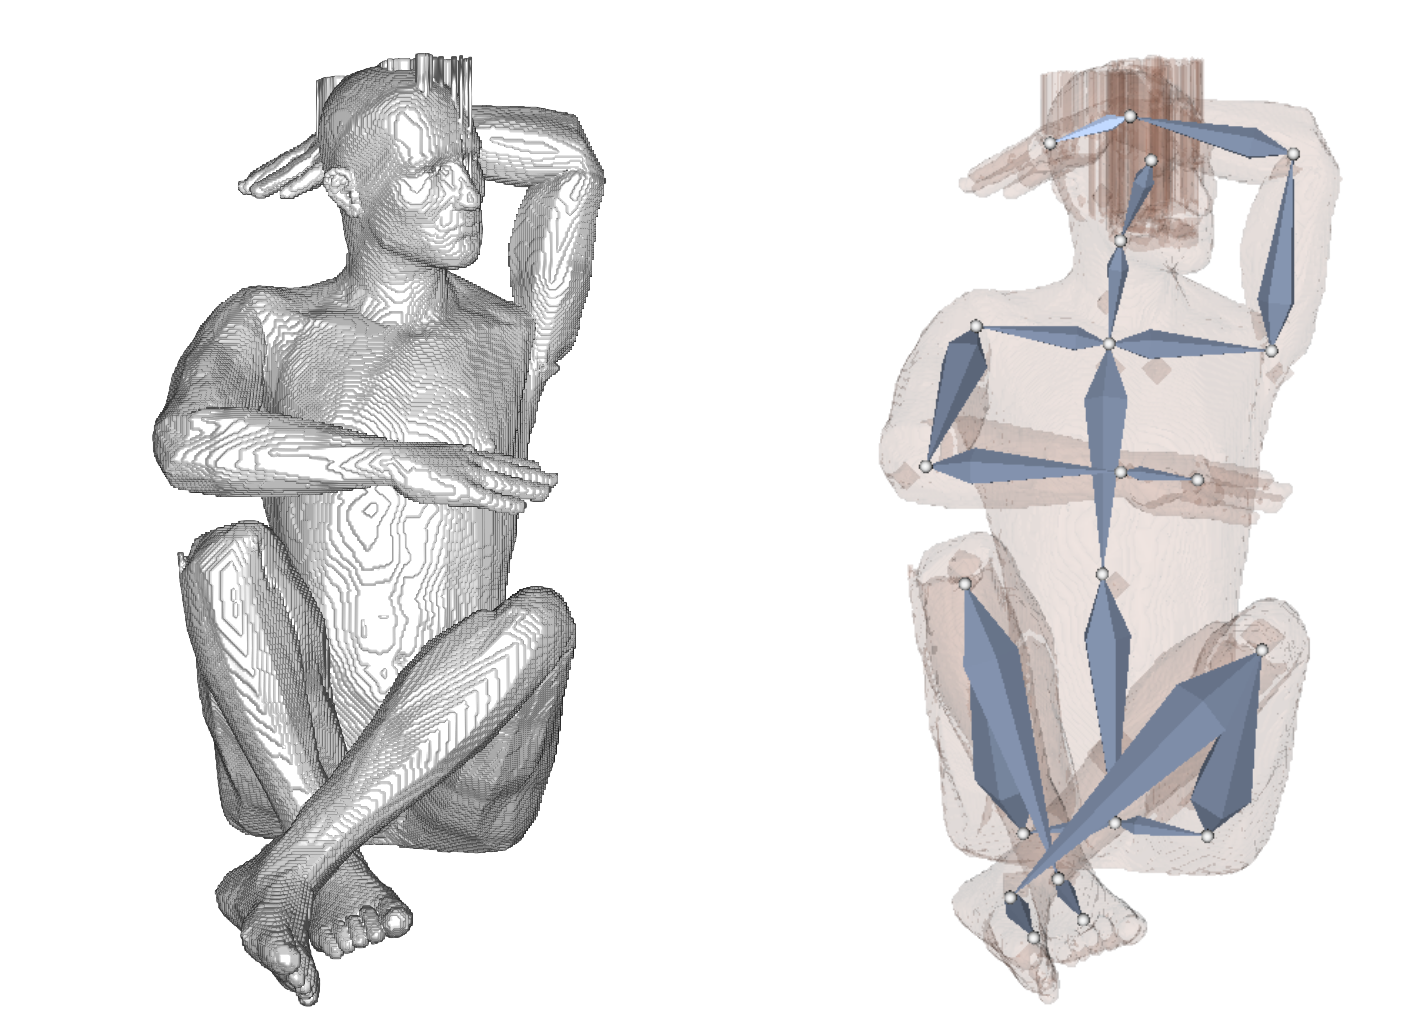
\includegraphics[width=13cm]{content/images/results/man6Front.png}
	\caption{Front view of the sisxth fetus pose. On the left the volume visualization of the prototype and on the right the visualization of the included armature.}
	\label{fig:}
\end{figure}
\begin{figure} [htb!]
    \centering
	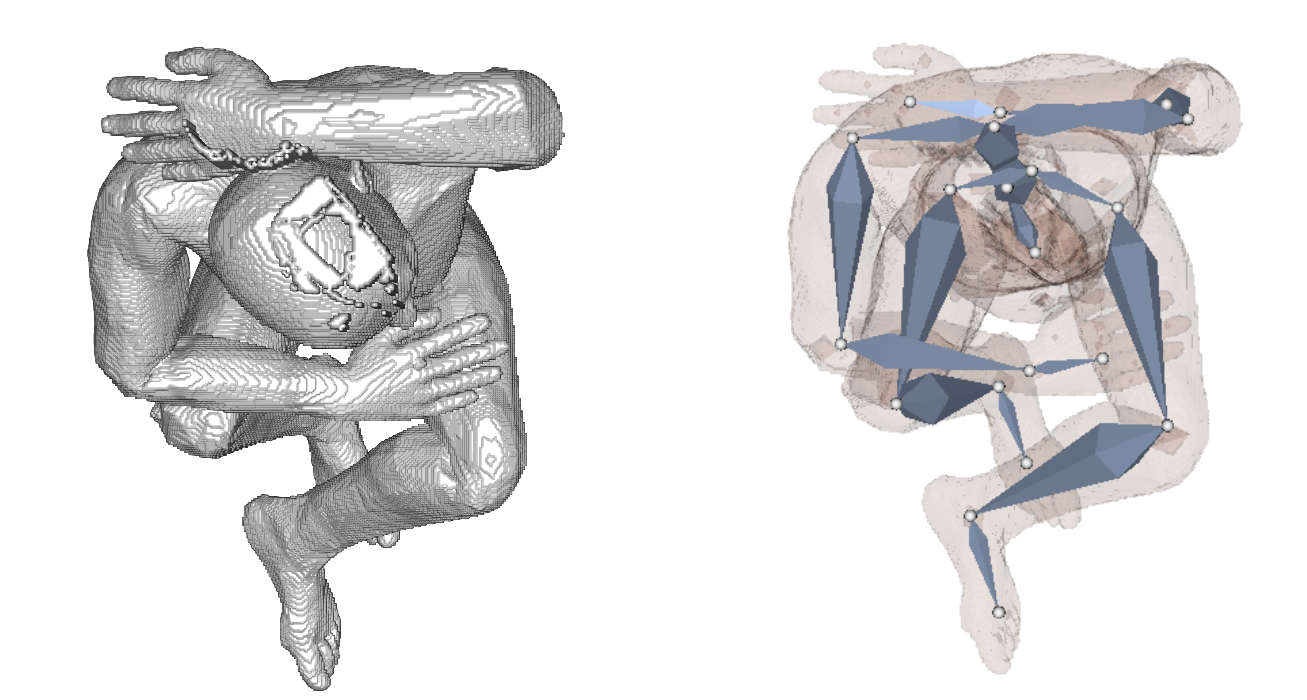
\includegraphics[width=13cm]{content/images/results/man6Top.png}
	\caption{Top view of the same formation also volume and armature view.}
	\label{fig:}
\end{figure}

\begin{figure} [htb!]
    \centering
	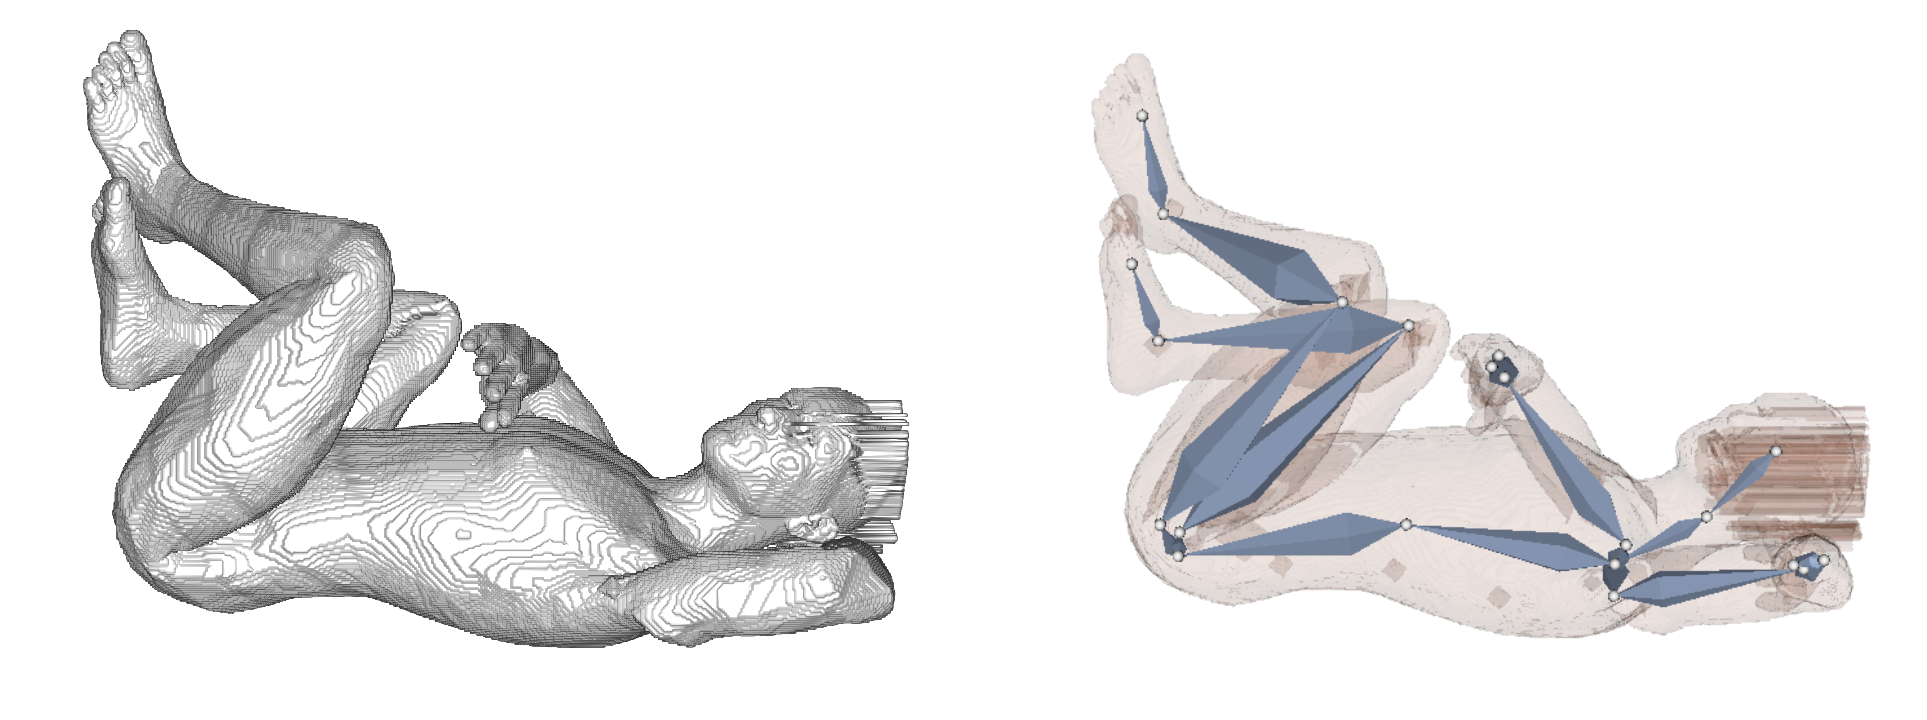
\includegraphics[width=15cm]{content/images/results/man6Side.png}
	\caption{Side view of the pose also with visible armature and volume visualization.}
	\label{fig:}
\end{figure}
\vspace{3cm}
\begin{figure} [htb!]
    \centering
	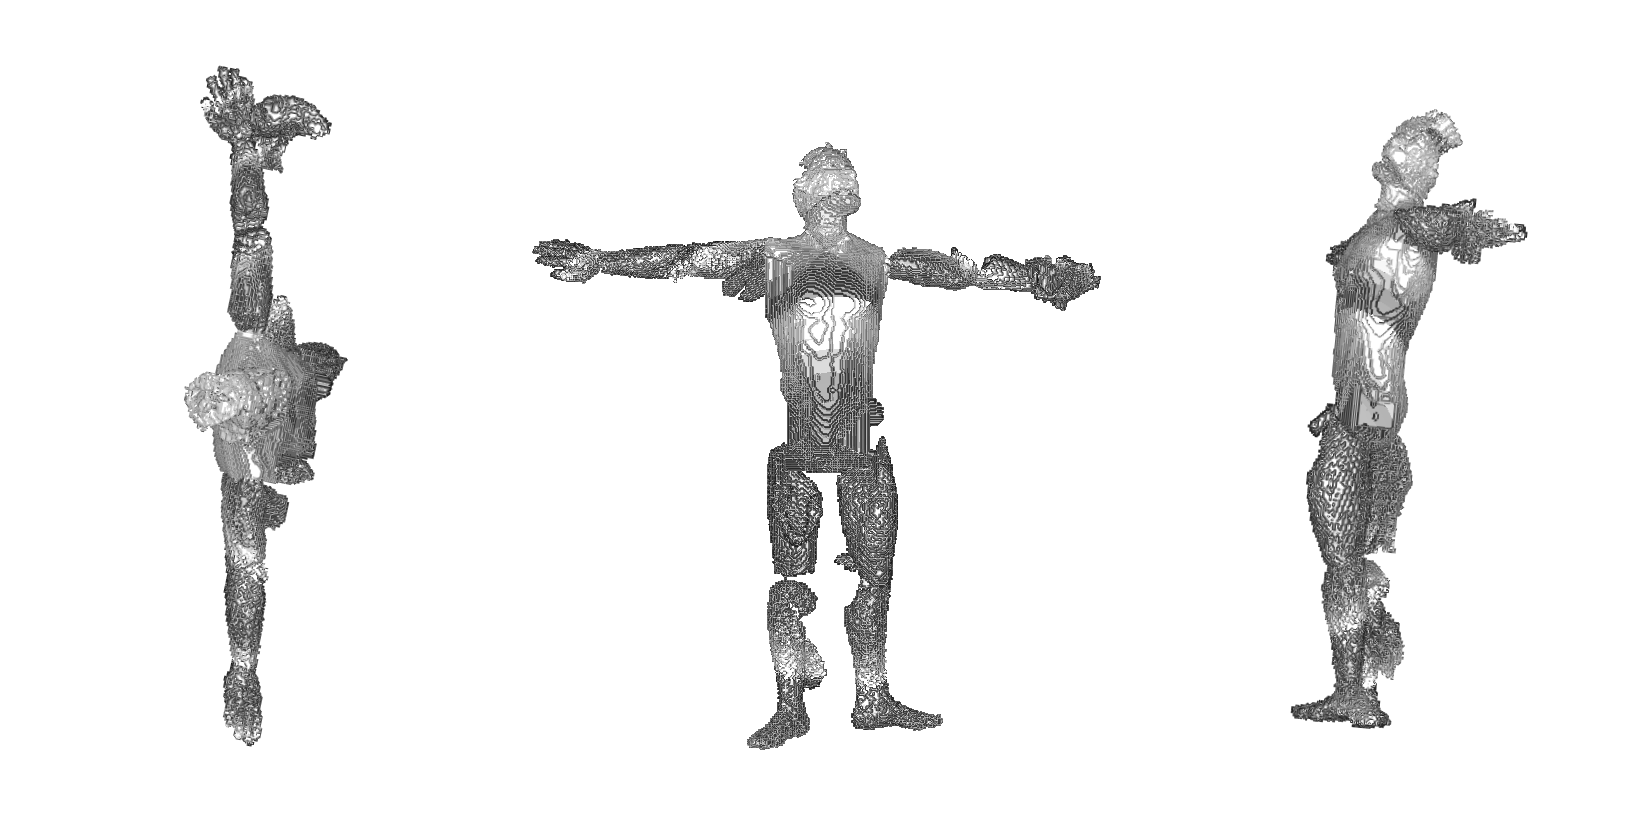
\includegraphics[width=16cm]{content/images/results/man6Result.png}
	\caption{The result T-pose of the sixth fetus pose from left to right: Top view, front view and side view.}
	\label{fig:}
\end{figure}

%% START MAN 7
\newpage
\begin{figure} [htb!]
    \centering
	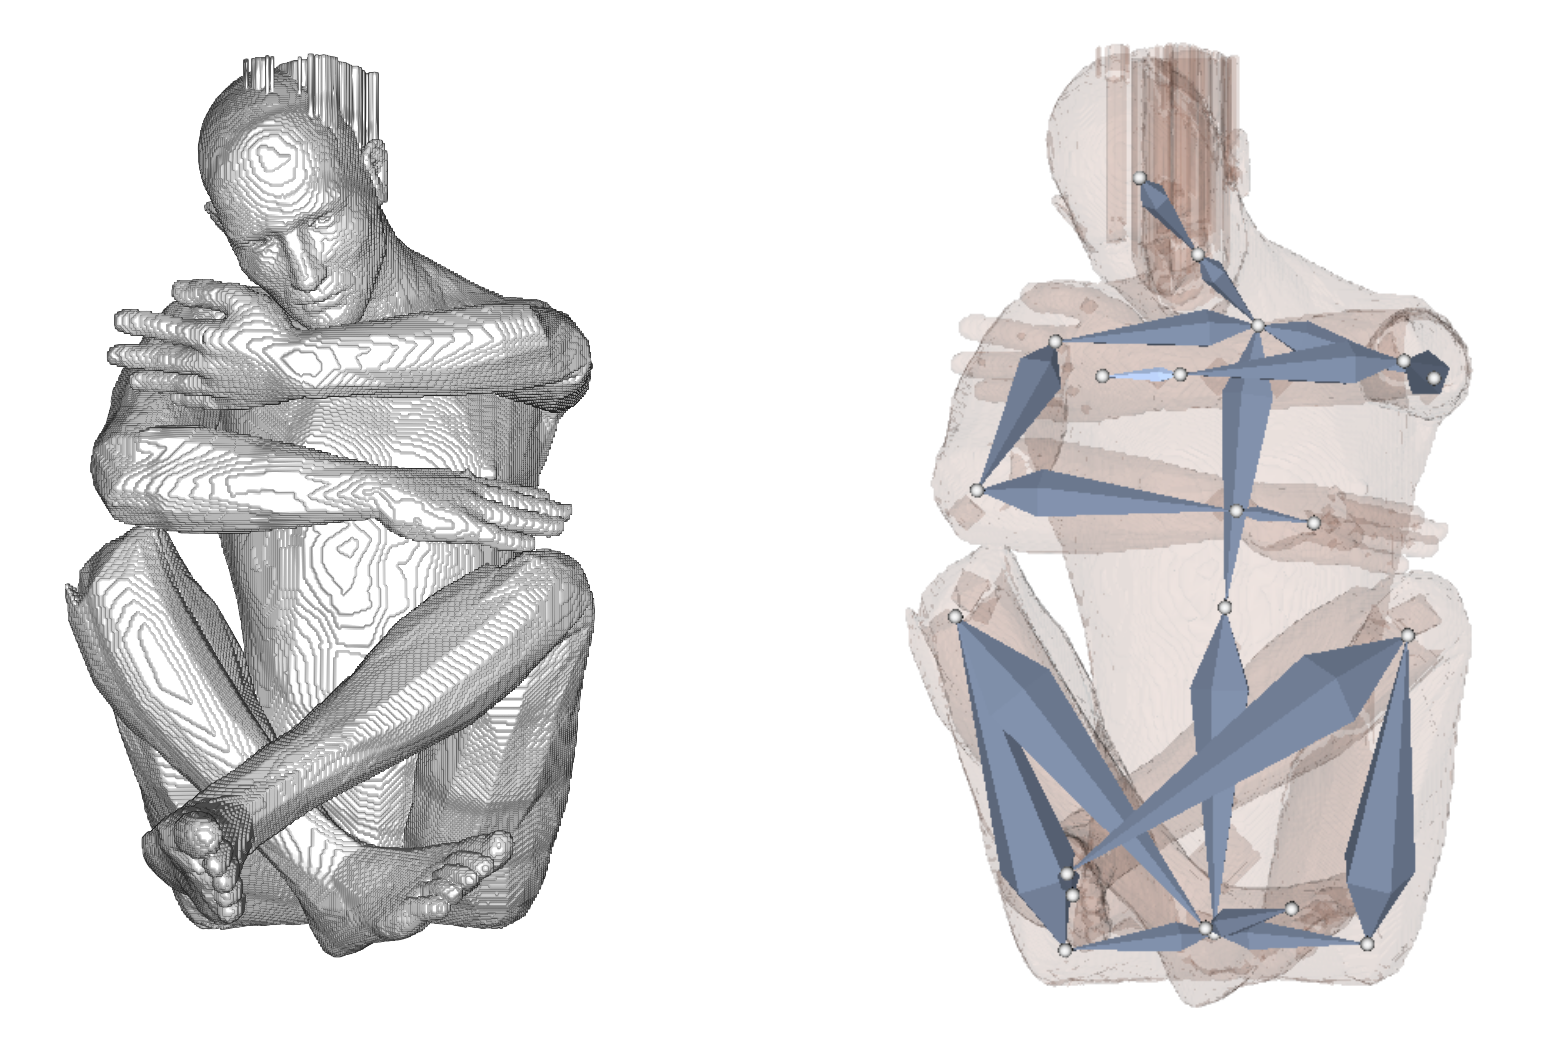
\includegraphics[width=13cm]{content/images/results/man7Front.png}
	\caption{Front view of the seventh fetus pose. On the left the volume visualization of the prototype and on the right the visualization of the included armature.}
	\label{fig:}
\end{figure}
\begin{figure} [htb!]
    \centering
	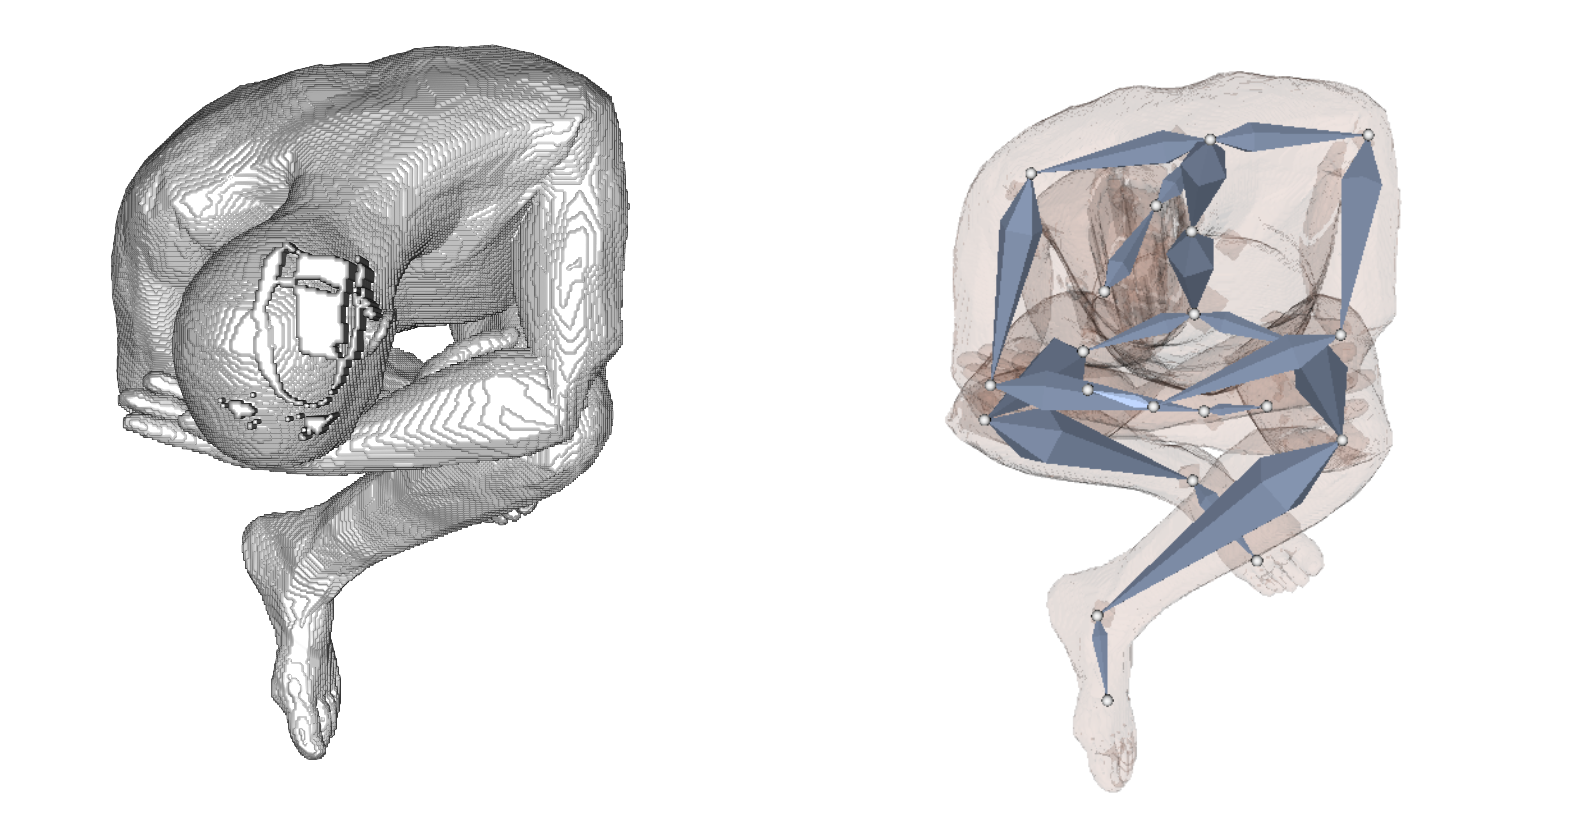
\includegraphics[width=13cm]{content/images/results/man7Top.png}
	\caption{Top view of the same formation also volume and armature view.}
	\label{fig:}
\end{figure}

\begin{figure} [htb!]
    \centering
	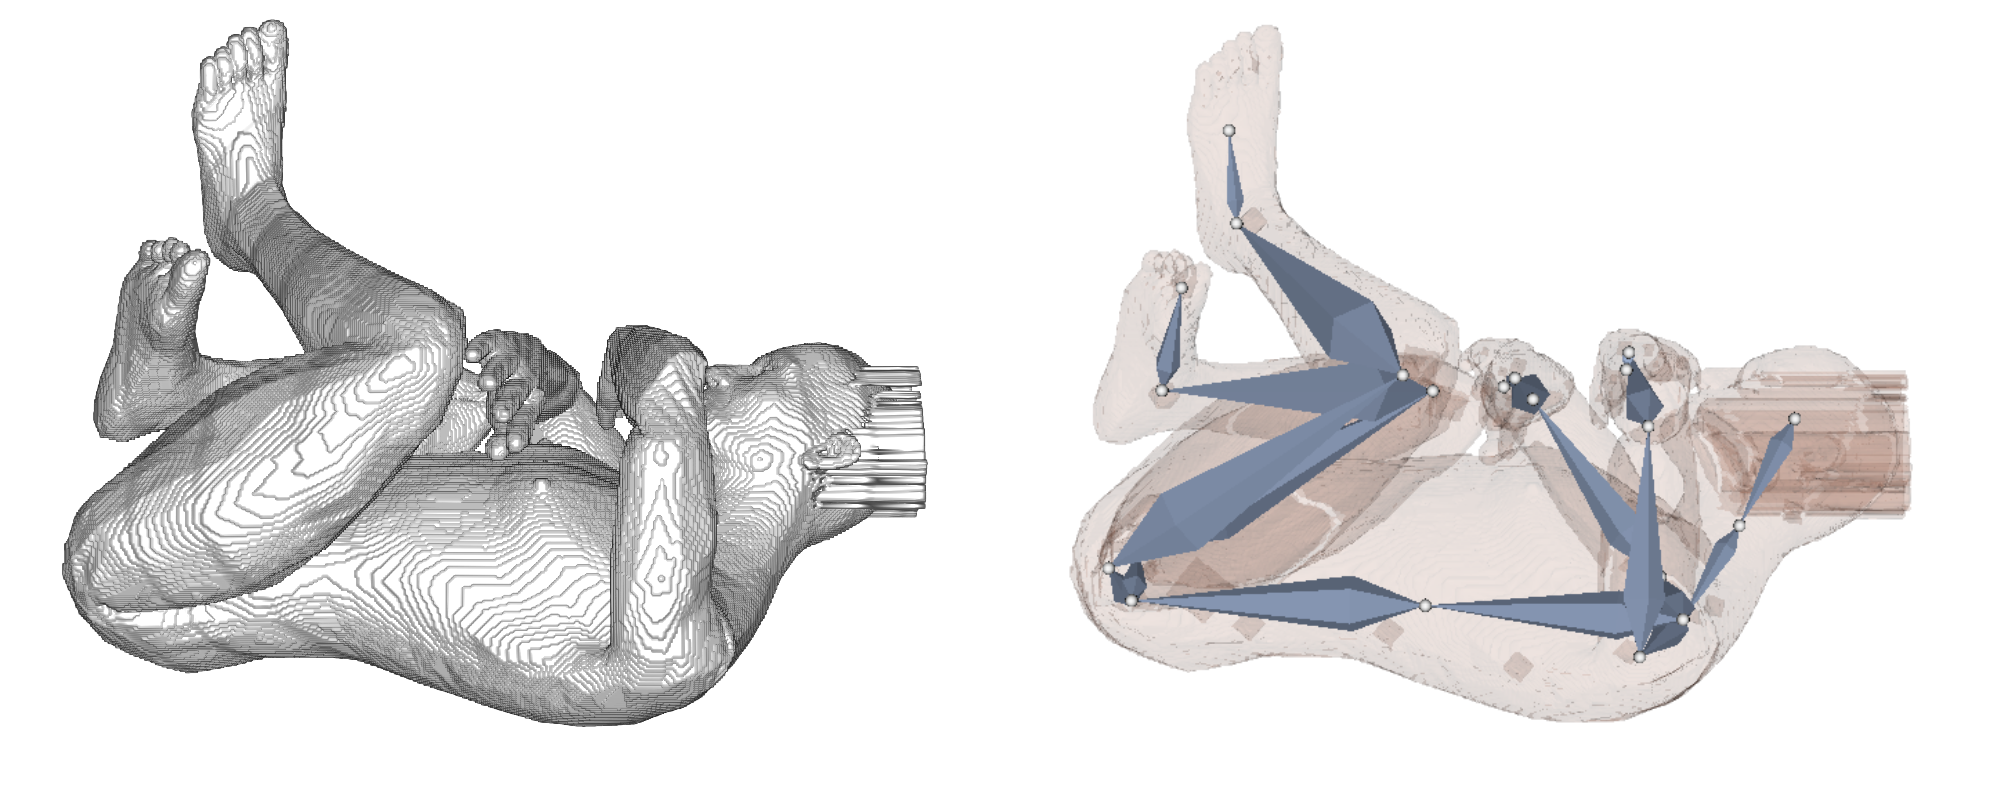
\includegraphics[width=15cm]{content/images/results/man7Side.png}
	\caption{Side view of the pose also with visible armature and volume visualization.}
	\label{fig:}
\end{figure}
\vspace{3cm}
\begin{figure} [htb!]
    \centering
	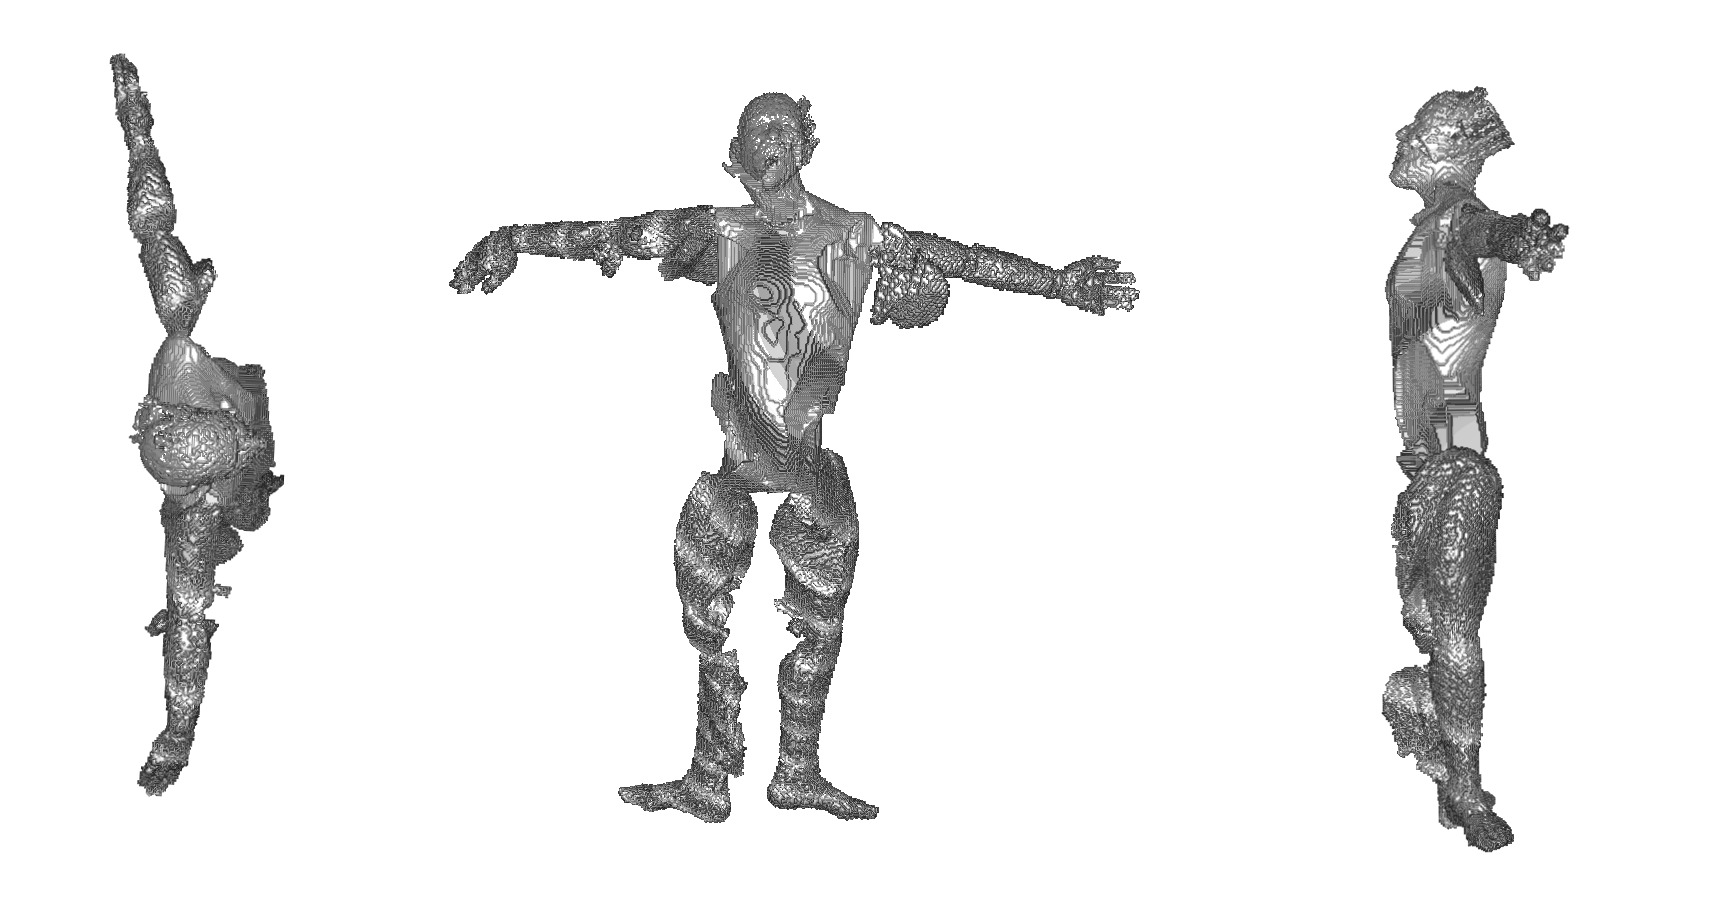
\includegraphics[width=16cm]{content/images/results/man7Results.png}
	\caption{The result T-pose of the seventh fetus pose from left to right: Top view, front view and side view.}
	\label{fig:}
\end{figure}

\clearpage
\subsubsection{Performance statistics}
As stated in the begin of this chapter performance analysis is importing when presenting a novel method or approach and therefore we tried to measure how good the algorithm performs. The performance is measured using different operations. First there is a time consuming part involved in the process of having the T-pose transformed data namely the rigging, described in \ref{sct:rigging}. Therefore the time being spent in the program Blender \cite{Foundation2019Blender} has been measured from the step of loading the data until the result has been saved for further processing. The overview of the times is shown in Table \ref{tbl:duration}. The average duration of the whole process being done in Blender is \textbf{seven} Minutes. The rigging is performed by the author and therefore maybe someone less familiar would perform slower. 

\begin{table}[!htb]
    \centering
    \begin{tabular}{l|l|l|l}
    Phantom & Starting time & End time & Duration \\ \hline
    Man1    & 15:12         & 15:24    & 00:12    \\ \hline
    Man2    & 16:46         & 16:50    & 00:04    \\ \hline
    Man3    & 15:41         & 15:52    & 00:11    \\ \hline
    Man4    & 16:12         & 16:21    & 00:09    \\ \hline
    Man5    & 16:24         & 16:30    & 00:06    \\ \hline
    Man6    & 16:32         & 16:36    & 00:04    \\ \hline
    Man7    & 16:38         & 16:44    & 00:06   
    \end{tabular}
    \caption{Overview of the duration needed to rig the seven phantom models.}
    \label{tbl:duration}
\end{table}

The second and maybe most important measurement of performance is how well the transformed data represent the original T-pose. Therefore the result has been registered with the T-pose input and the scalar volume difference has been produced. The result of one of those measurements is shown in Figure \ref{fig:differences}. It somehow looks like that there is lots of data left and therefore the overlapping is low, but it has to be considered that the data is volumetric and therefore the number of voxels remaining is important and not if the rest still looks like a human. The analysis results are presented in Table \ref{tbl:performance}. The average of the overlap percentage is \textbf{}{79,02\%} which depends on how well the armature is placed in the data.
 
\begin{figure} [htb!]
	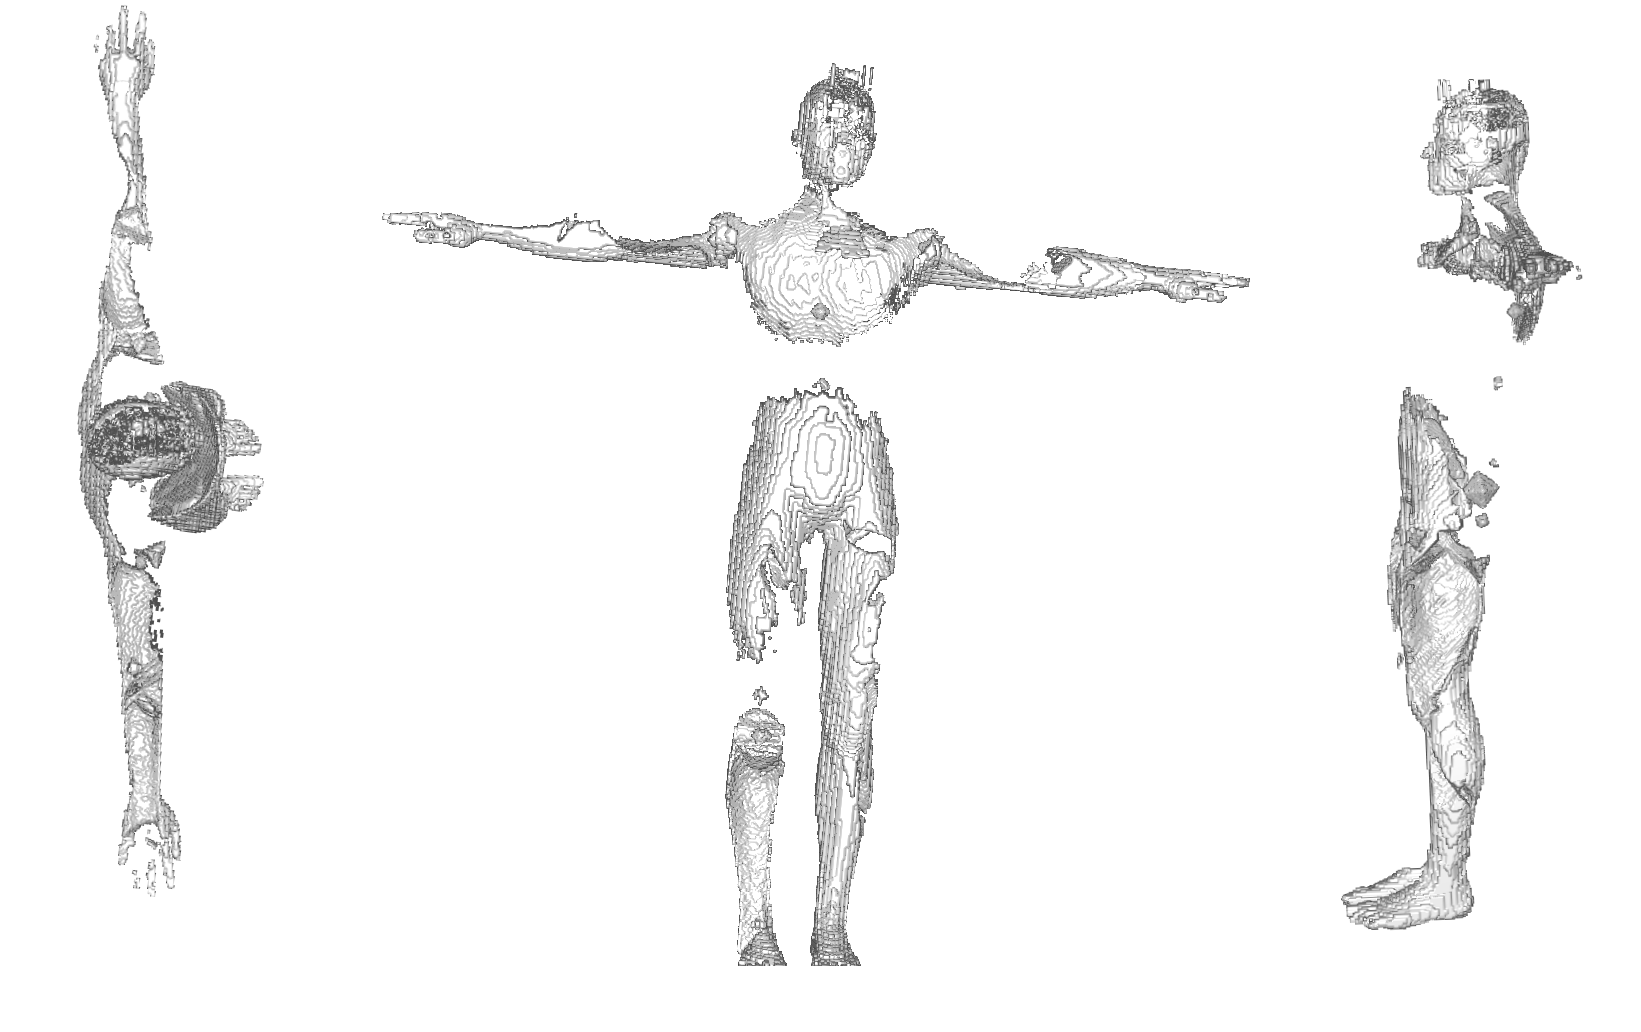
\includegraphics[width=14cm]{content/images/results/man4Differences}
	\caption{The result of the difference of the fourth fetus pose from left to right: Top view, front view and side view.}
	\label{fig:differences}
\end{figure}

\begin{table}[!htb]
    \centering
    \begin{tabular}{l|l|l|l}
    \begin{tabular}[c]{@{}l@{}}Total amount\\ voxels T-pose\end{tabular} & \begin{tabular}[c]{@{}l@{}}Amount of voxels\end{tabular}\\\begin{tabular}[c]{@{}l@{}}Percentage of voxels\\left after subtraction\end{tabular} & Percentage Left & Percentage Overlap \\ \hline
    2654642 & 790637 & 29,78\% & 70,22\% \\ \hline
    2654642 & 886471 & 33,39\% & 66,61\% \\ \hline
    2654642 & 572079 & 21,55\% & 78,45\% \\ \hline
    2654642 & 530825 & 20,00\% & 80,00\% \\ \hline
    2654642 & 492437 & 18,55\% & 81,45\% \\ \hline
    2654642 & 286991 & 10,81\% & 89,19\% \\ \hline
    2654642 & 338764 & 12,76\% & 87,24\%           
    \end{tabular}
    \caption{The table shows the total amount of voxels in the T-pose and the amount of voxels left after subtraction of the result of the method and the T-pose. The left two columns }
    \label{tbl:performance}
\end{table}

\clearpage
\subsection{Fetus data}
The fetus data presented in this section is also gathered from the internet. One dataset is a simple \gls{3d} model of a fetus \cite{SpecialboyBebyModel} and the other one a simulation of a whole fetus ultrasound scan produced by Cortes et.al. \cite{Cortes2016UltrasoundEvaluation}. This section is structured just as the one with the man phantoms. The difference between the datasets is that in this case there is no ground truth that can be compared so there is no T-pose which is the right solution. Therefore the only performance analysis can be done in terms of time needed for rigging the data.

\begin{figure} [htb!]
    \centering
	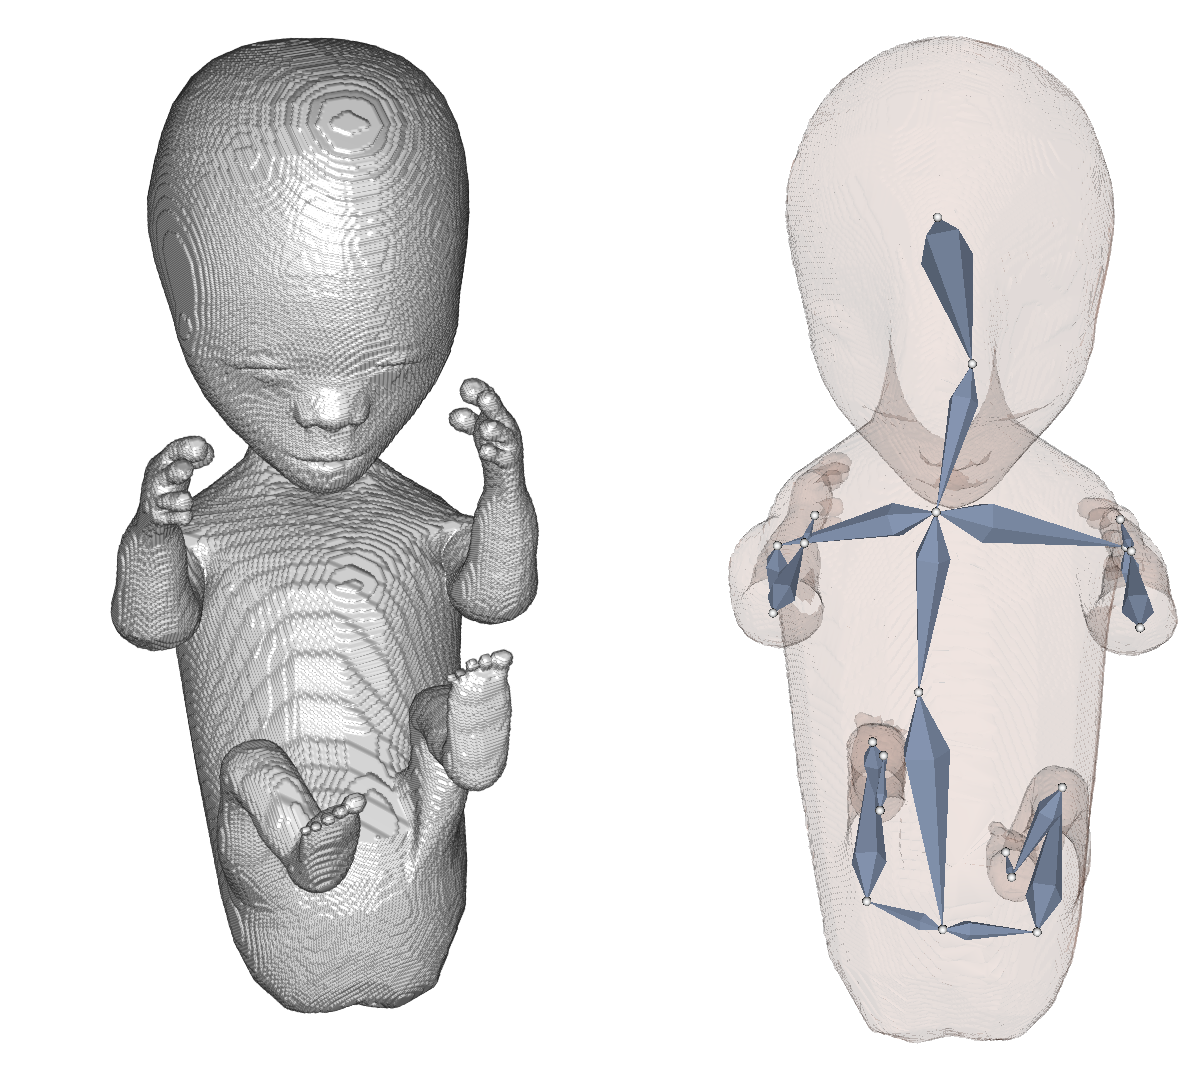
\includegraphics[width=11cm]{content/images/results/fetusModelFront.png}
	\caption{Front view of the fetus model \cite{SpecialboyBebyModel}. On the left the volume visualization of the prototype and on the right the visualization of the included armature.}
	\label{fig:}
\end{figure}
\begin{figure} [htb!]
    \centering
	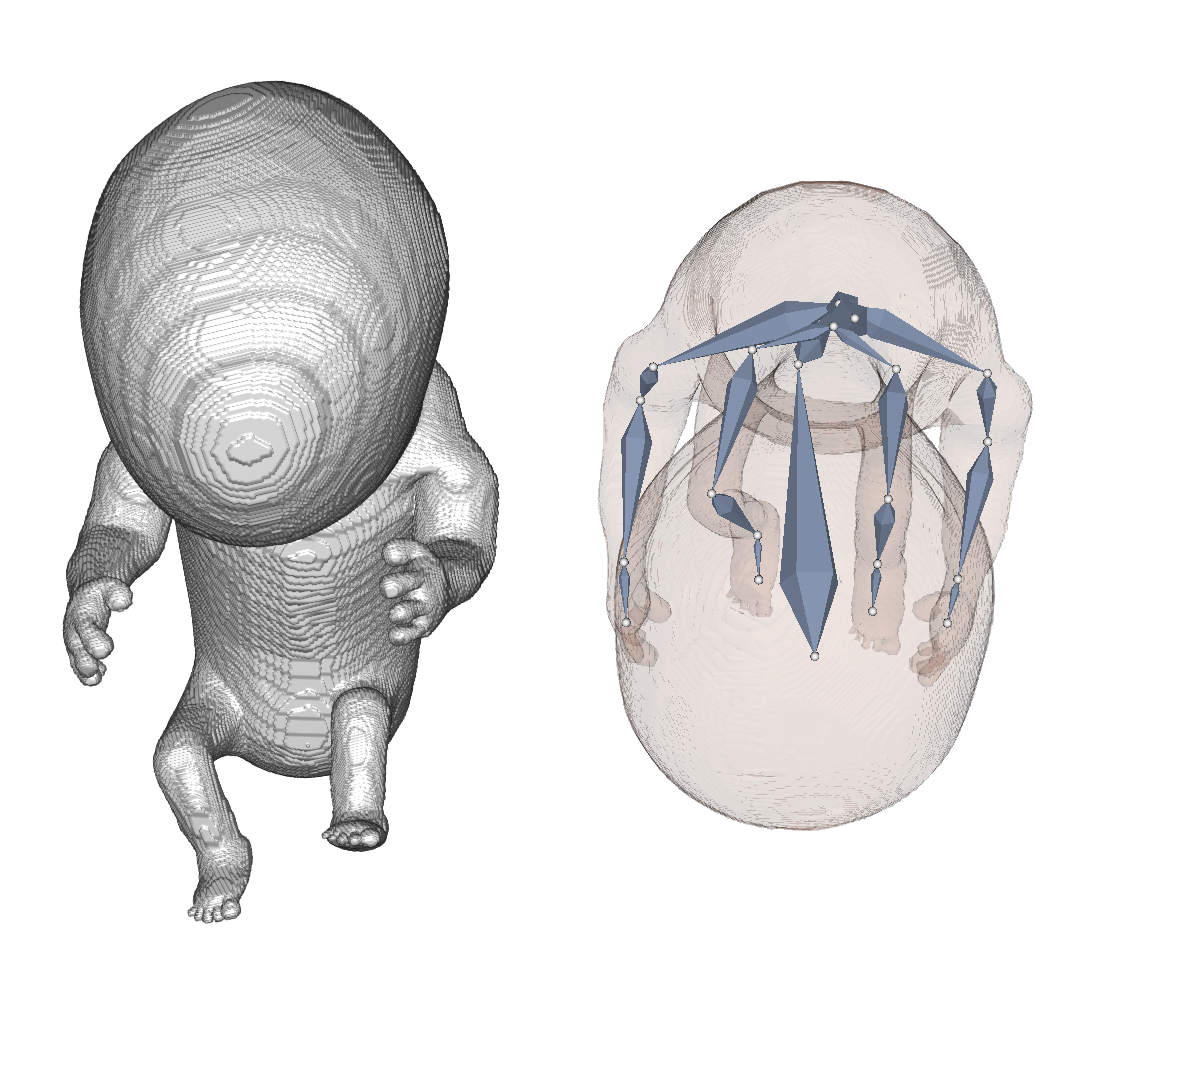
\includegraphics[width=13cm]{content/images/results/fetusModelTop.png}
	\caption{Top view of it also volume and armature view.}
	\label{fig:}
\end{figure}
\begin{figure} [htb!]
    \centering
	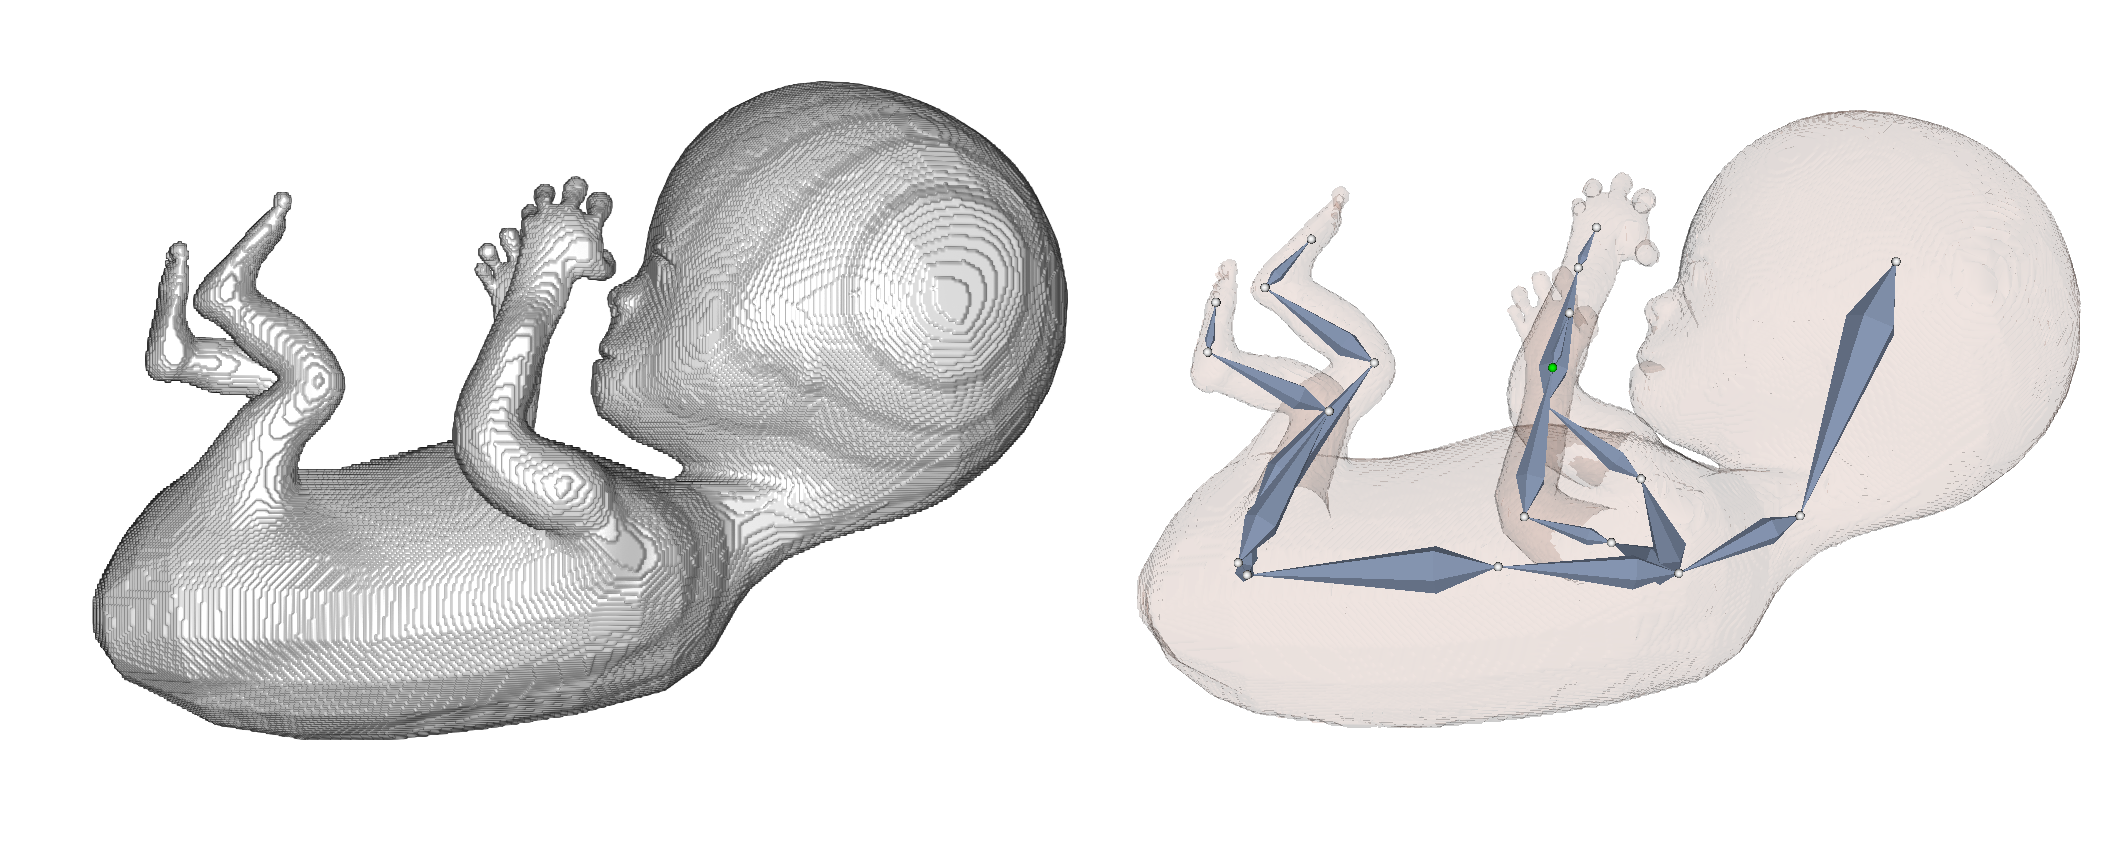
\includegraphics[width=14cm]{content/images/results/fetusModelSide.png}
	\caption{Side view of the pose also with visible armature and volume visualization.}
	\label{fig:}
\end{figure}
\begin{figure} [htb!]
    \centering
	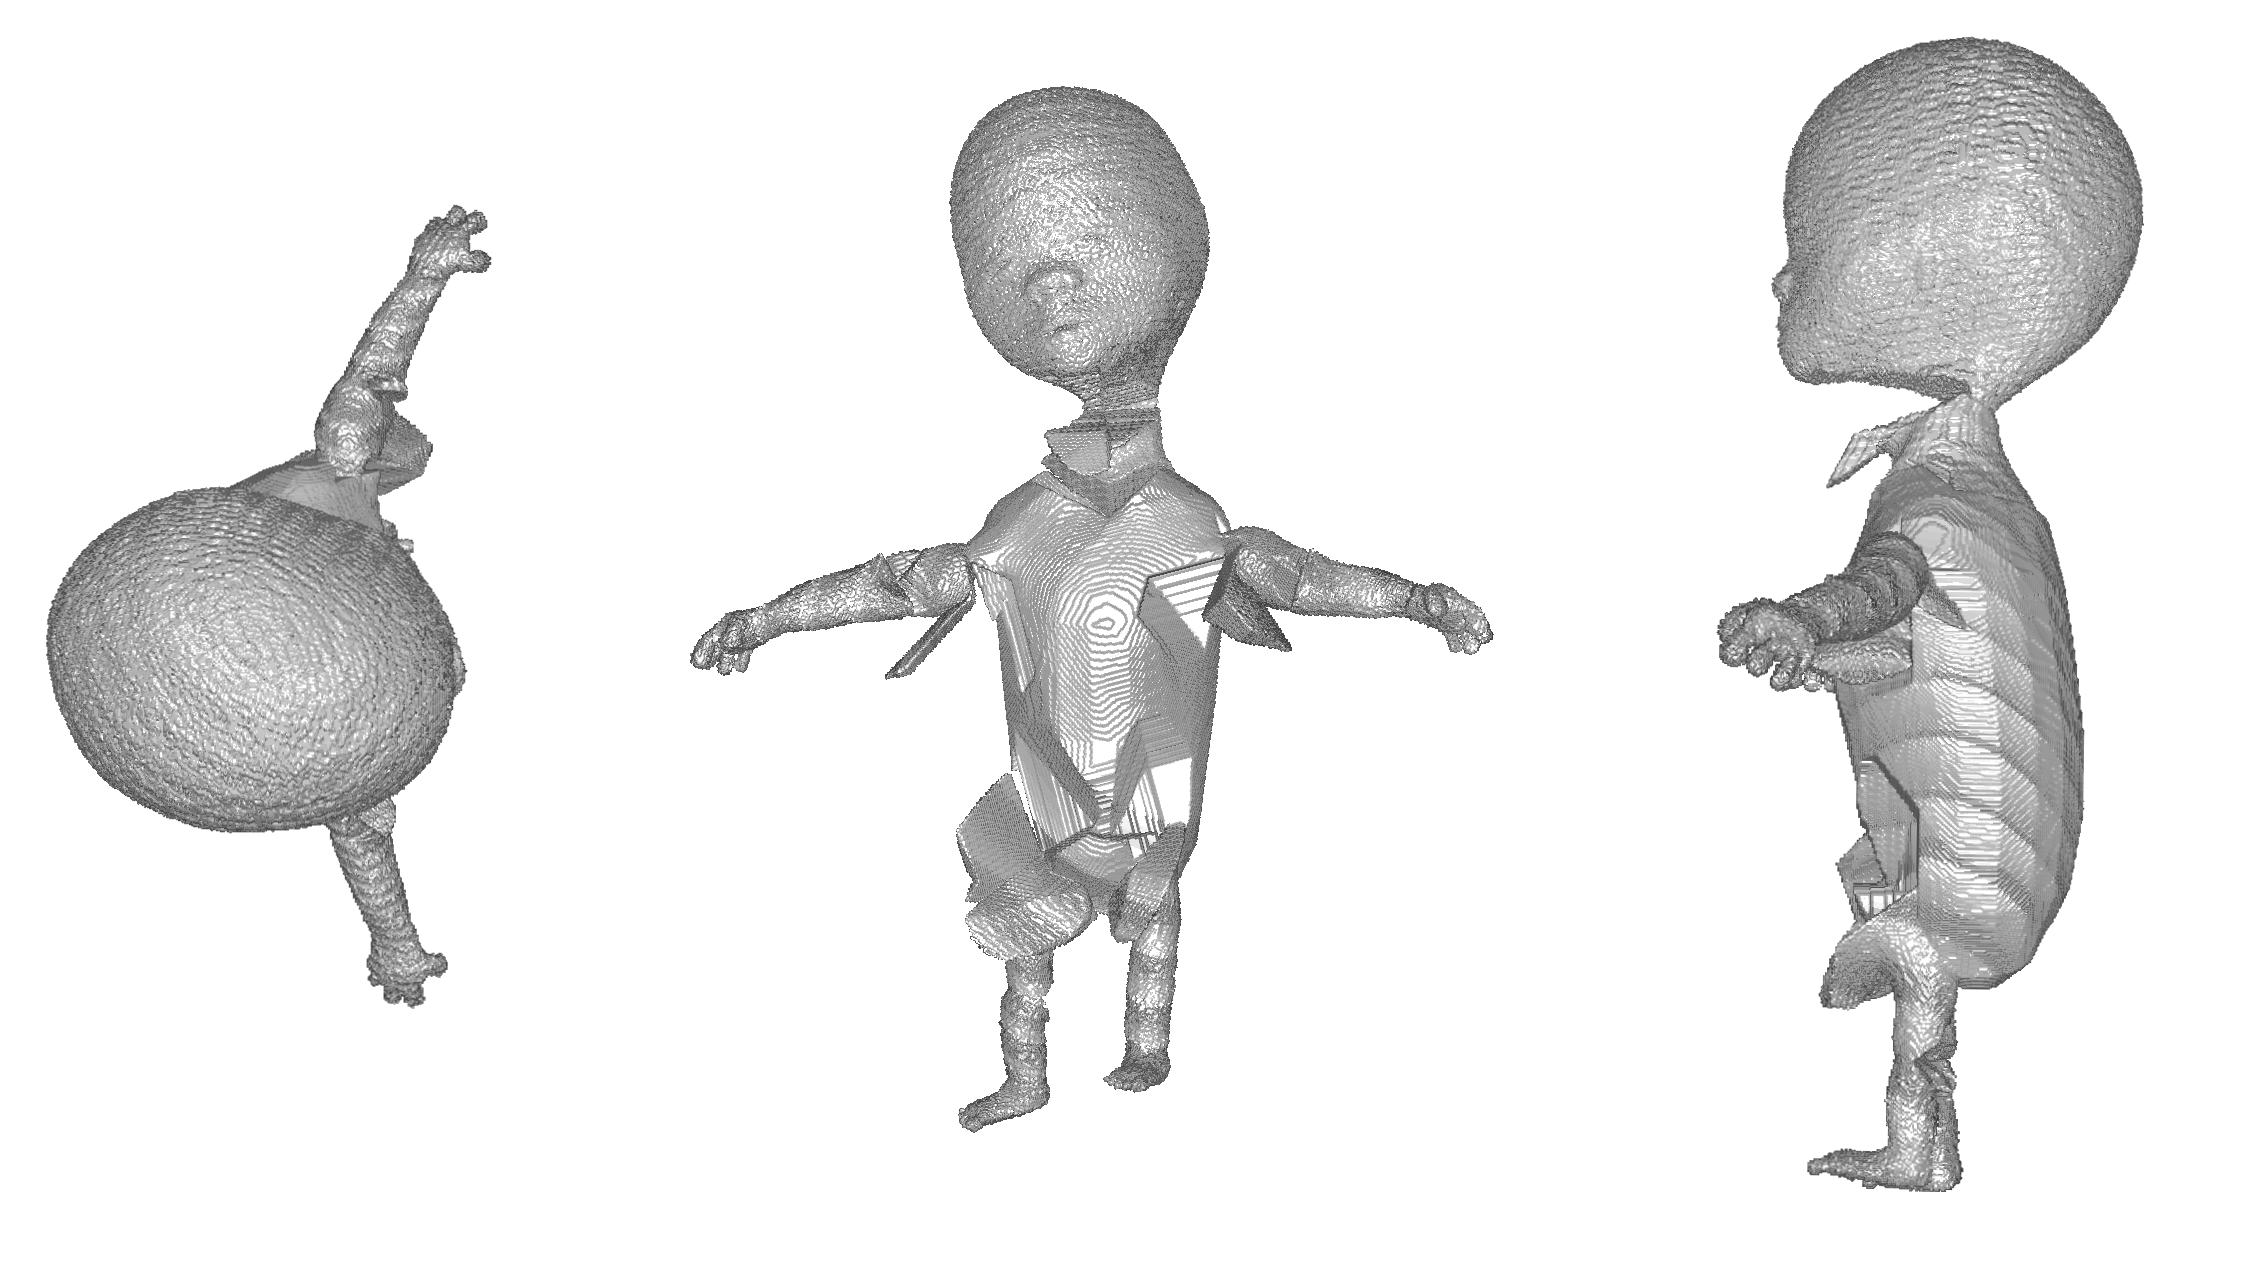
\includegraphics[width=14cm]{content/images/results/fetusModelResult.png}
	\caption{The result T-pose of the fetus model from left to right: Top view, front view and side view.}
	\label{fig:}
\end{figure}
\newpage

The following data shows the phantom model which represents how the output of a full fetus ultrasound scan may look like. The data has been pre-filtered in order to make is usable for the method presented. The original data is shown in Figure \ref{fig:phantomFetusOriginalData}.

\begin{figure} [htb!]
    \centering
	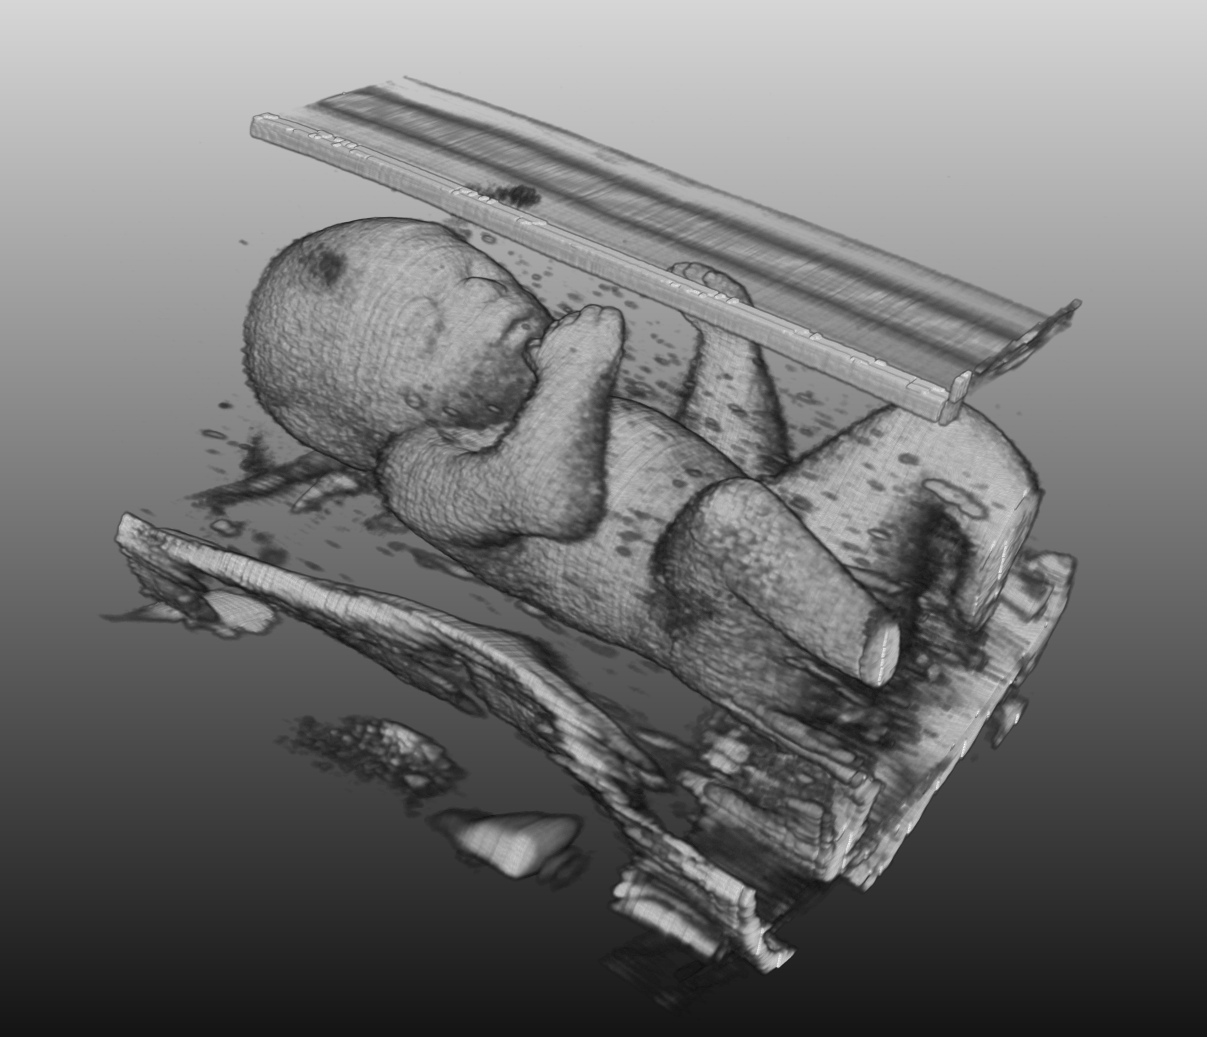
\includegraphics[width=8cm]{content/images/phantomFetusOr.PNG}
	\caption{Original phantom model created by Cortes \cite{Cortes2016UltrasoundEvaluation} which represents a phanom of a full fetus \gls{3d} ultrasound scan.}
	\label{fig:phantomFetusOriginalData}
\end{figure}

The result of the preprocessing step and the result of the fetus formation is shown here.
\begin{figure} [htb!]
    \centering
	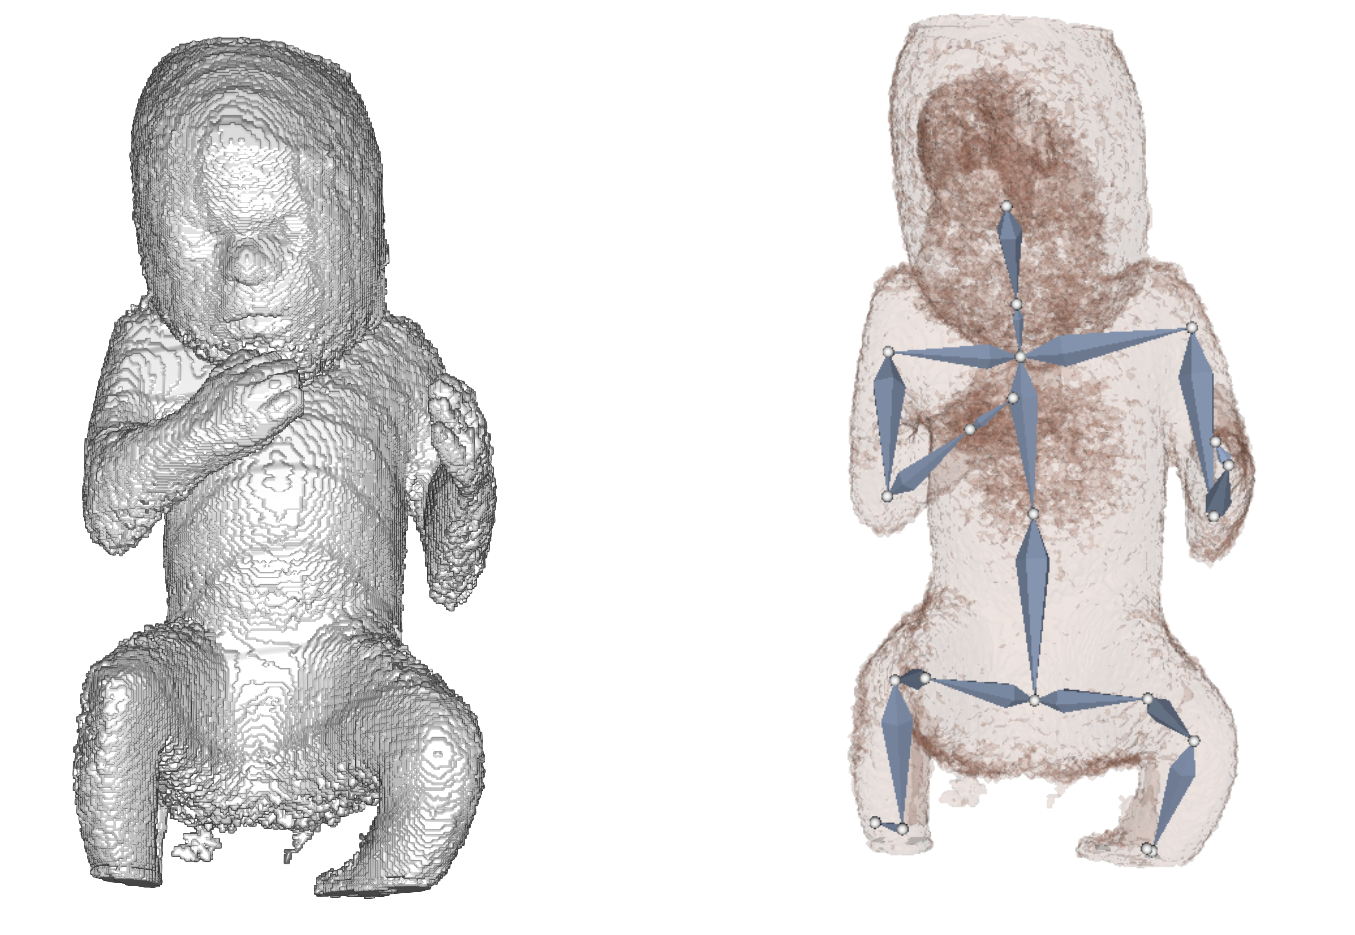
\includegraphics[width=13cm]{content/images/results/fetusPhantomFront.png}
	\caption{Front view of the fetus phantom provided by Cortes \cite{Cortes2016UltrasoundEvaluation}. On the left the volume visualization of the prototype and on the right the visualization of the included armature.}
	\label{fig:}
\end{figure}
\begin{figure} [htb!]
    \centering
	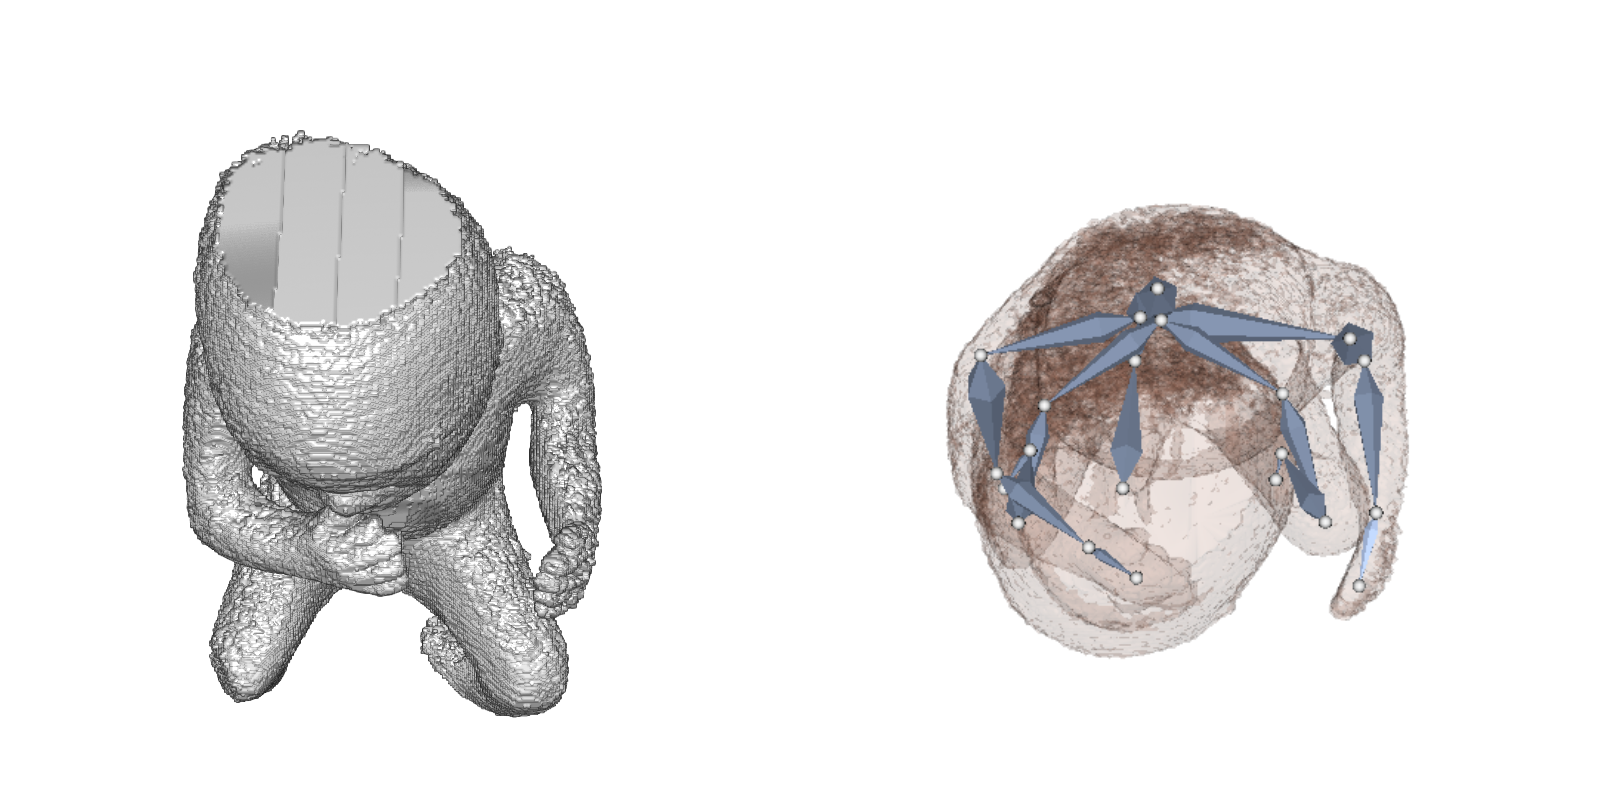
\includegraphics[width=13cm]{content/images/results/fetusPhantomTop.png}
	\caption{Top view of the phantom also volume and armature view.}
	\label{fig:}
\end{figure}
\begin{figure} [htb!]
    \centering
	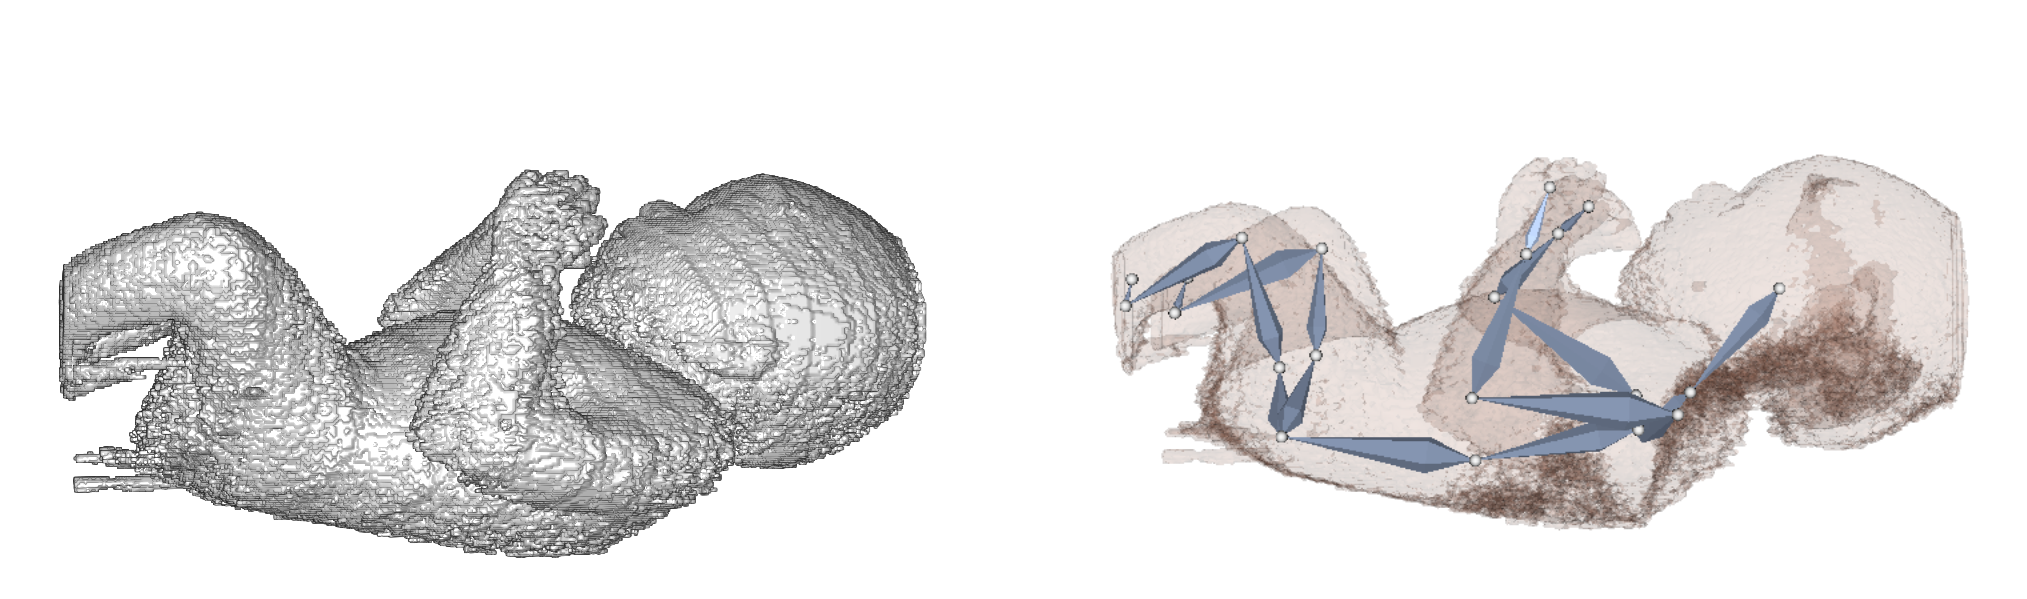
\includegraphics[width=15cm]{content/images/results/fetusPhantomSide.png}
	\caption{Side view of the pose also with visible armature and volume visualization.}
	\label{fig:}
\end{figure}
\begin{figure} [htb!]
    \centering
	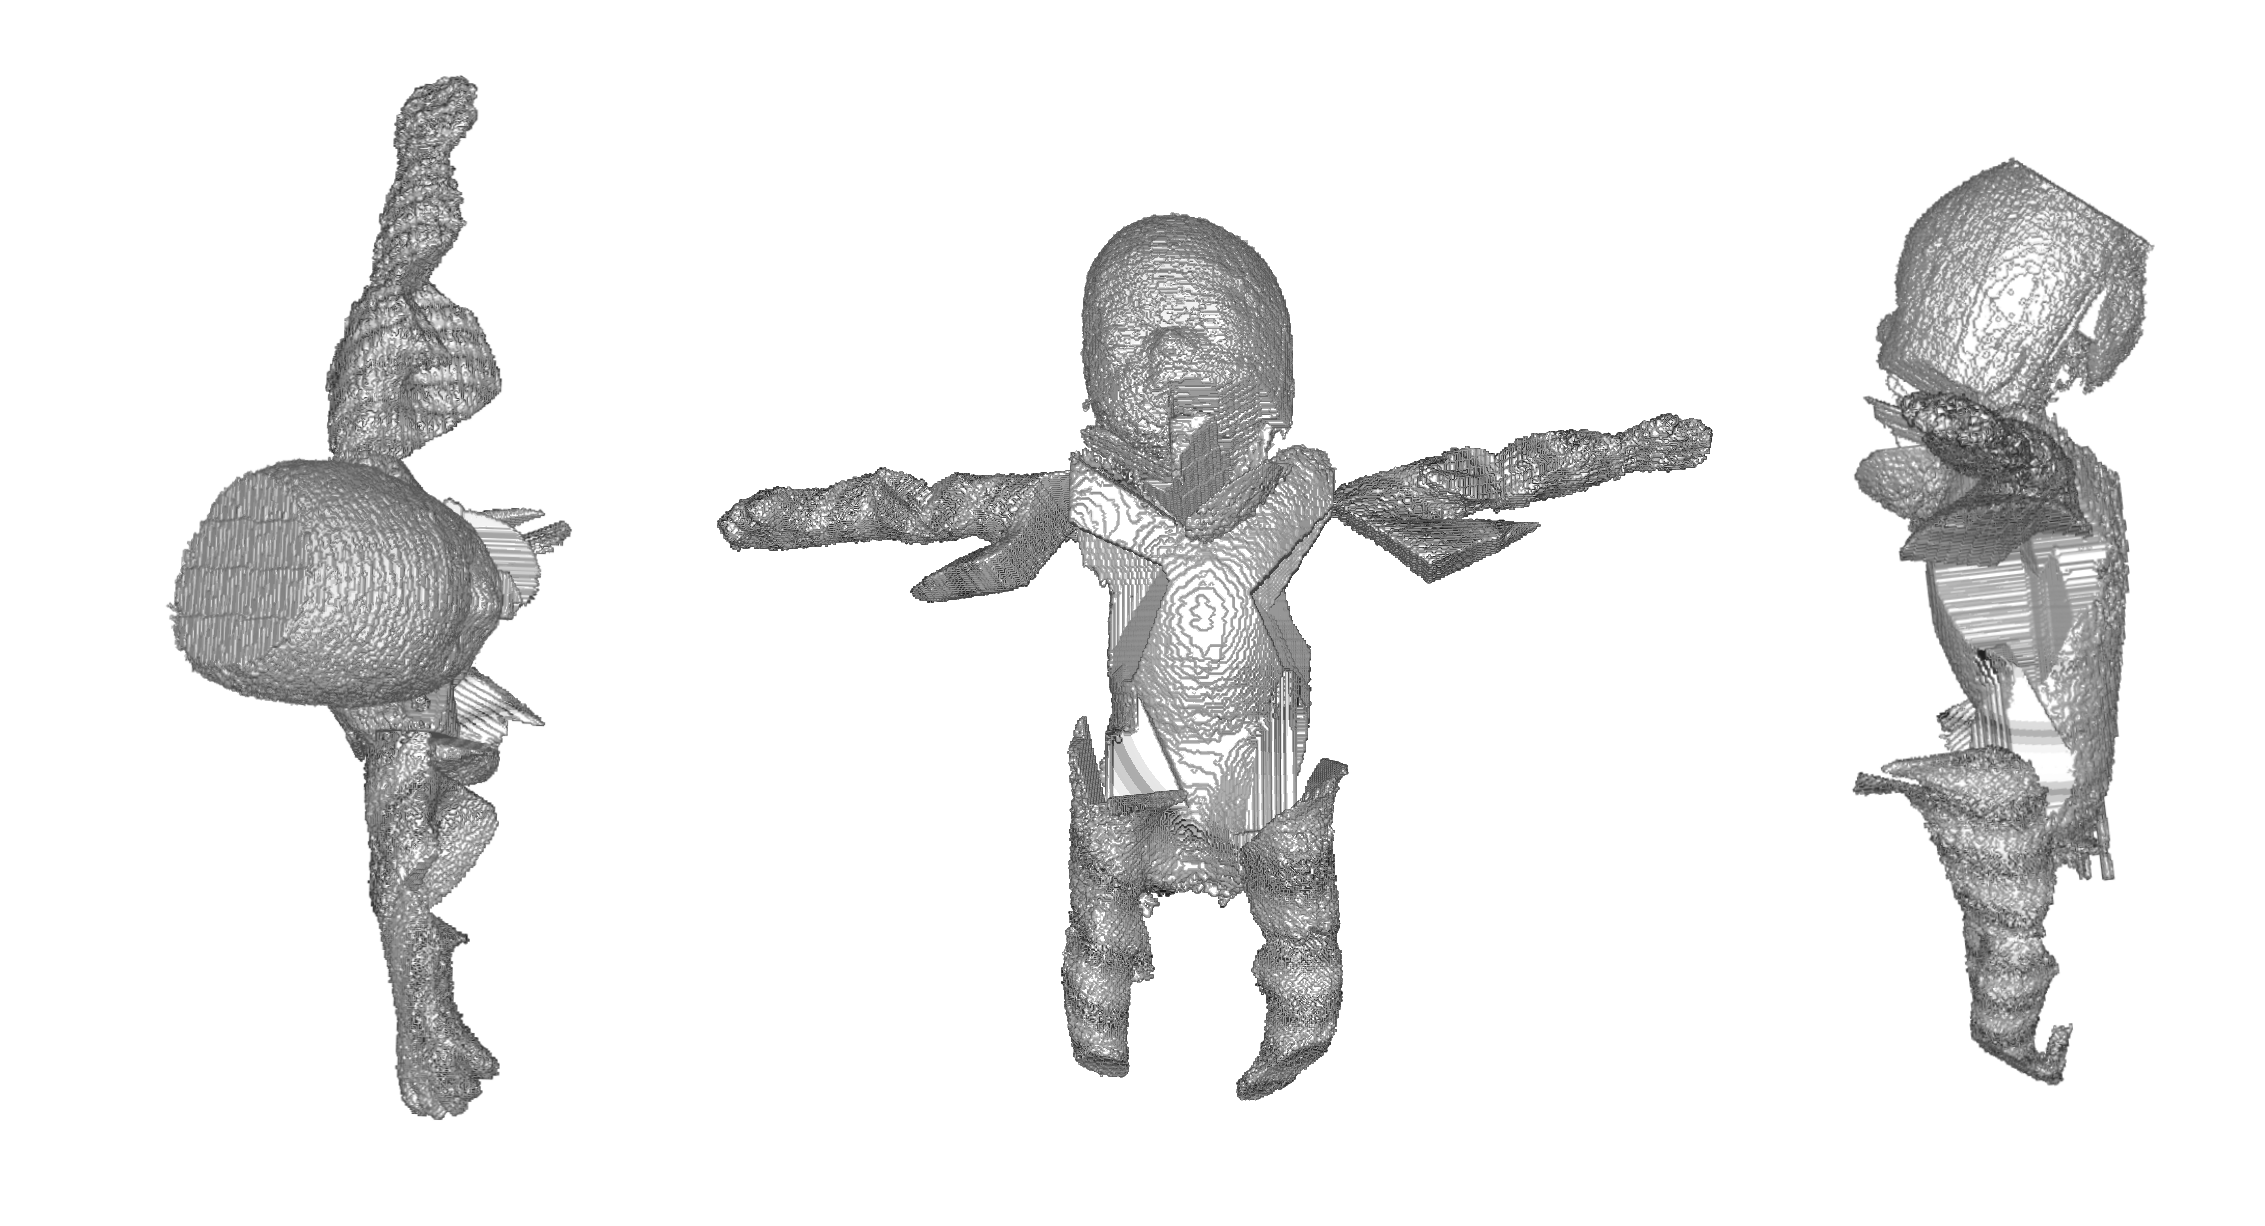
\includegraphics[width=16cm]{content/images/results/fetusPhantumResult.png}
	\caption{The result T-pose of the fetus phantom from left to right: Top view, front view and side view.}
	\label{fig:}
\end{figure}

\clearpage
The analysis of the method in terms of fetus like or phantom fetus model is represented by the time the end user needs in order to perform the manual step of rigging. Table \ref{tbl:fetusPerformance} represents the time needed to perform this manual step. The average time to do so is \textbf{eight} minutes.

\begin{table}[!htb]
    \centering
    \begin{tabular}{l|l|l|l}
                   & Starting time & End time & Duration \\\hline
    Fetus Model     & 18:50         & 18:56    & 00:06    \\\hline
    Fetus US Phantom & 19:00         & 19:11    & 00:11   
    \end{tabular}
    \label{tbl:fetusPerformance}
    \caption{Table representing the time needed for rigging the fetus model and the fetus ultrasound phantom.}
\end{table}

\section{Influence analysis}
This section of the results handles findings which somehow show where the limits of the method are. There are some influences which lead to major artefacts and unwanted results. Those like limiting cases are  presented here.

\subsection{Noise}

The first problem which has been identified is the influence of noise in the data. In case of the phantom ultrasound investigation result created by Cortes et.al. \cite{Cortes2016UltrasoundEvaluation} noise which is usual for an ultrasound investigation has been added. If this data is directly loaded into the blender application the result looks like shown in Figure \ref{fig:noiseVies} and Figure \ref{fig:noise3D}. This data cannot be used in order to rig the data and produce meaningful output. Therefore the preprocessing step has been established. The surrounding of the data has to be free of any noise. In fact the data representing the fetus itself may have some noise included which can be seen in the results of the fetus phantom.

\begin{figure} [htb!]
    \centering
	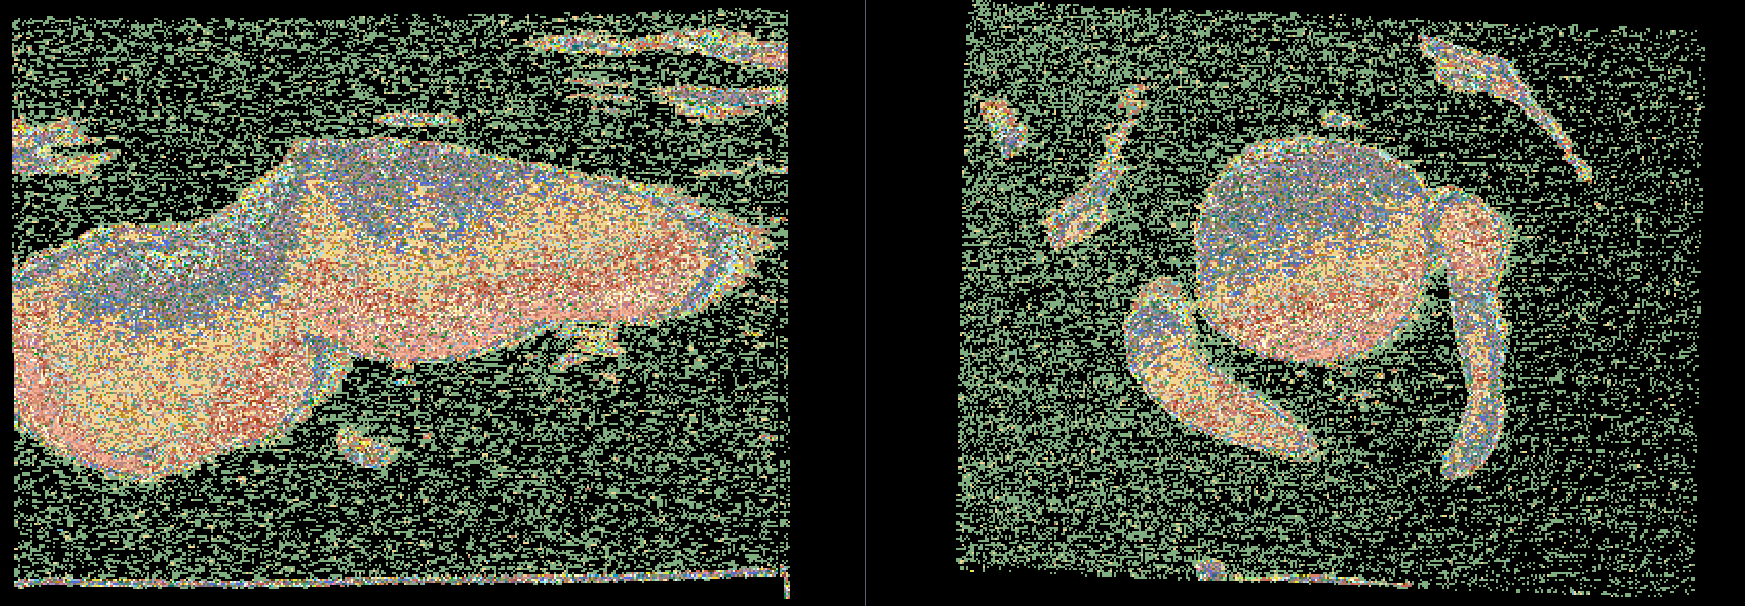
\includegraphics[width=13cm]{content/images/influence/viewsNoise.png}
	\caption{Different views of the noise in the phantom ultrasound data provided by Cortes et.al. \cite{Cortes2016UltrasoundEvaluation} in Bender \cite{Finet2014Bender:Morphing}.}
	\label{fig:noiseVies}
\end{figure}

\begin{figure} [htb!]
    \centering
	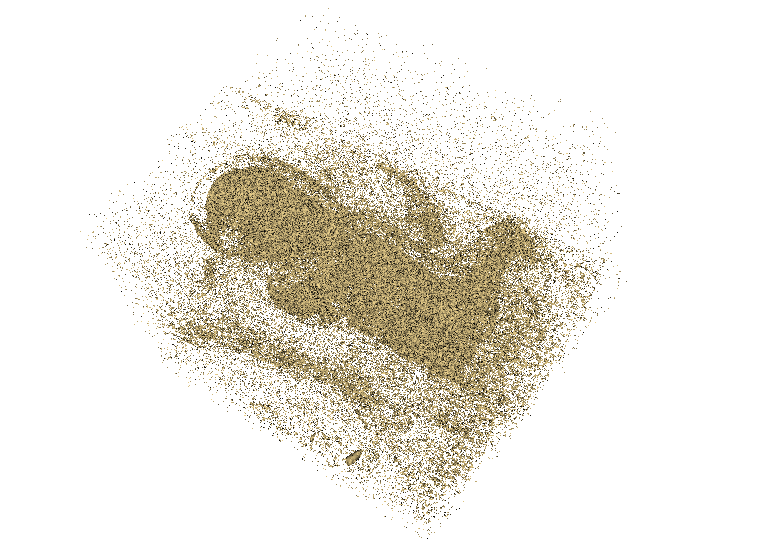
\includegraphics[width=13cm]{content/images/influence/noise3D.png}
	\caption{\gls{3d} visualisation of the fetus phantom with the noise included in Bender \cite{Finet2014Bender:Morphing}.}
	\label{fig:noise3D}
\end{figure}


\subsection{Weighting issues}

In some cases especially when the pose of the fetus is really packed and the limbs are very close to the body the weighting of the data does not perform very well. The problem is that if the arms are connected with the body the armature in the arms will compete with the armature in the body, namely the torso and the belly. The voxels in between those armature will be divided and the armature in the upper part will get a piece of the body which should not happen. Another example is given when the tighs are very close to he body they will somehow share some parts of the belly or of the pelvis. This phenomena is also likely to occur if the arms touch the legs. One example of this weighting issue is presented in Figure \ref{fig:weightingissue}.

\begin{figure} [htb!]
    \centering
	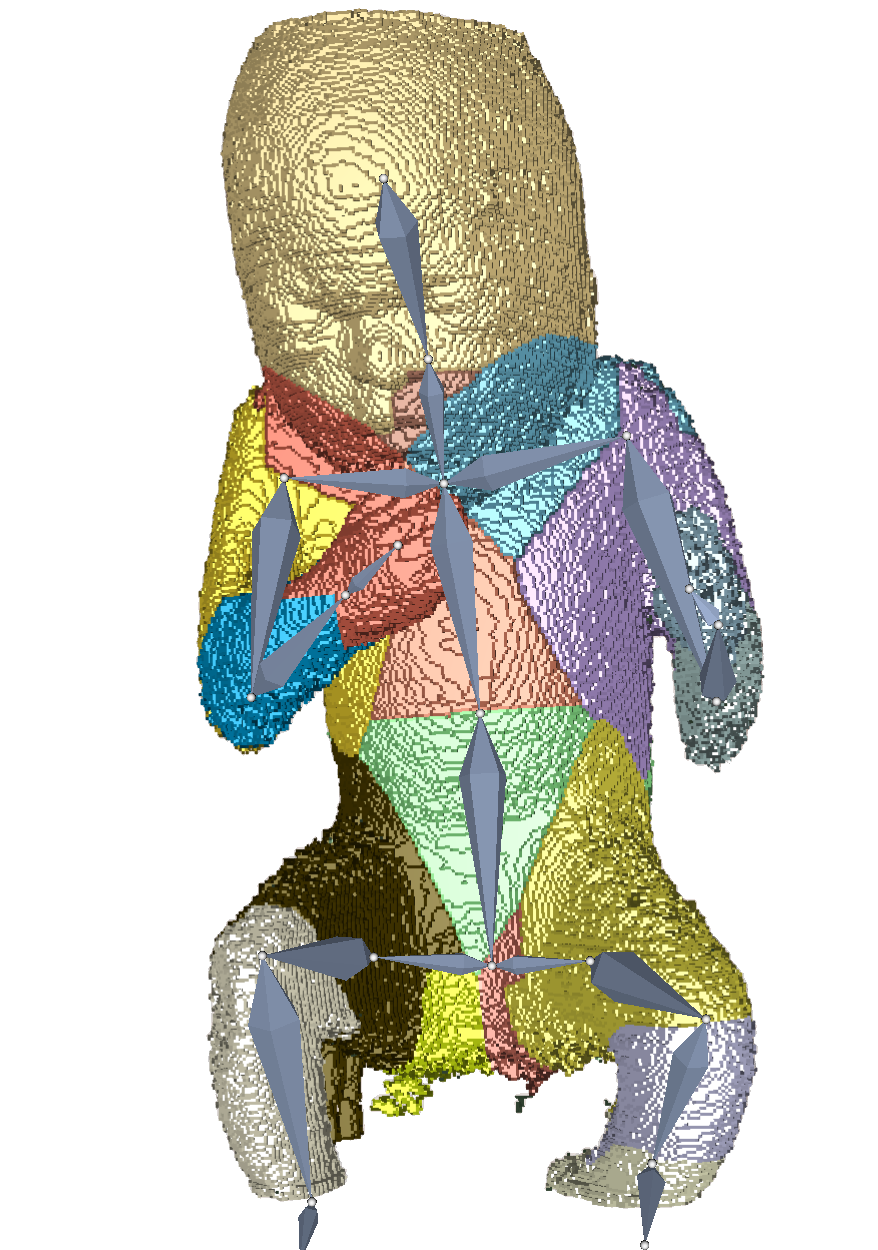
\includegraphics[width=9cm]{content/images/results/weightingIssues.png}
	\caption{Visualization of the weighting of the fetus phantom model. The arms and the legs have too much voxels assigned to them.}
	\label{fig:weightingissue}
\end{figure}

\newpage
\subsection{Limited space for rotation}

Another issue which has been faced during the evaluation phase was that the size of the volume to be worked with is somehow limited. The male phantom models have a resolution of 402x402 and around 250 in the depth which depends on the pose of the model. In order to perform all the rotations without limbs getting cut off by the volume borders first the volume is expanded by a factor of two which results in a volume size of around 800 times 800 and 500 in the depth. This is somehow also the limitation for the $threshold$ function in 3D Slicer. In some cases like the examples five, six and seven the expanding of the volume to the doubled size has not been enough. The initial result may be seen in Figure \ref{fig:rotationProblem}. If such datasets have to be analysed they have to be scaled down before they can be used. The scaling is done in case of  example five, six and seven and results in a lower resolution of the output.

\begin{figure} [htb!]
    \centering
	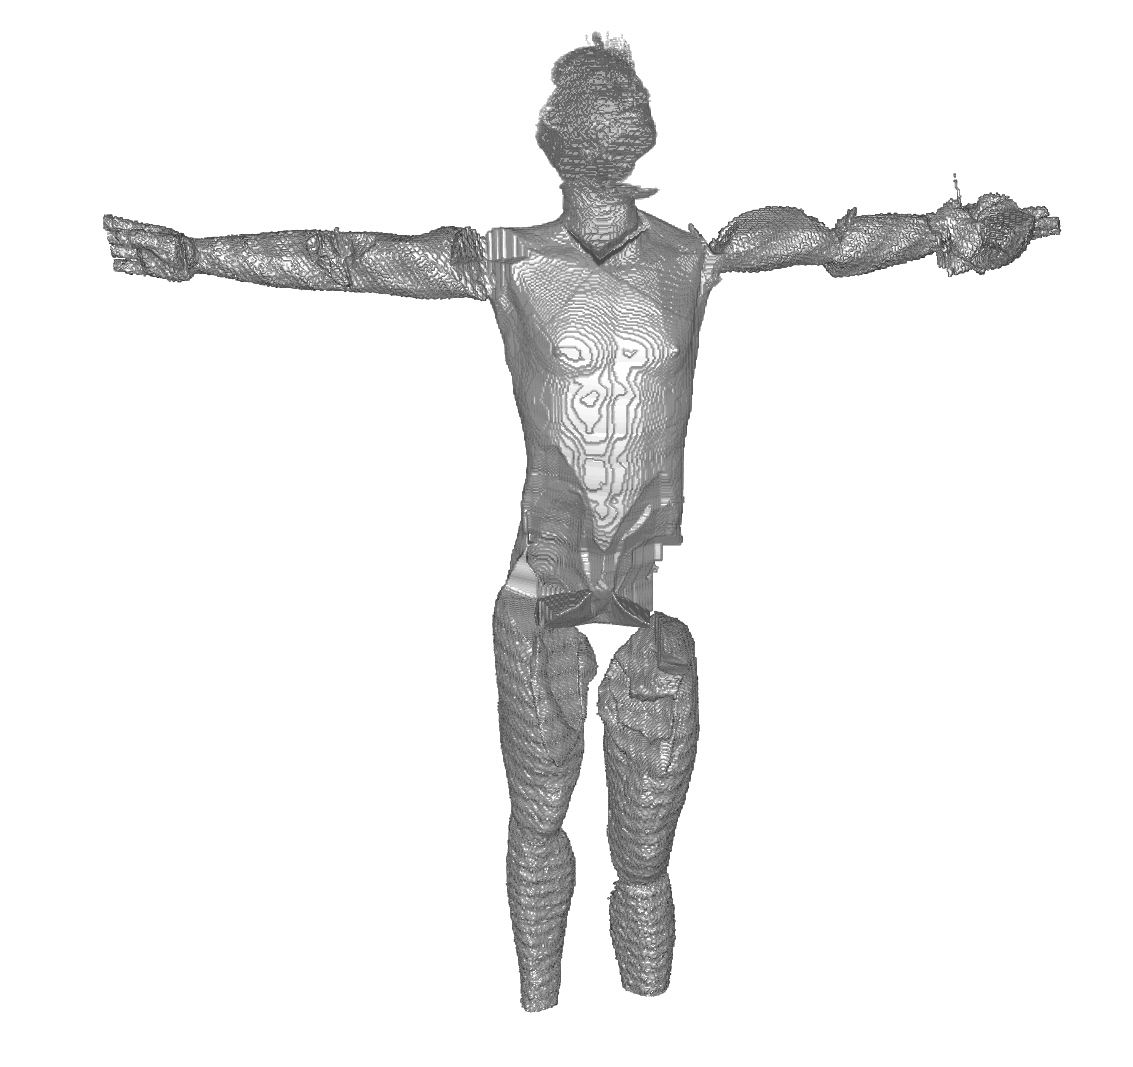
\includegraphics[width=14cm]{content/images/influence/rotationalProblem.png}
	\caption{The limited space for the rotation of the limbs leads to a cut off of the legs in case of the phantom man five}
	\label{fig:rotationProblem}
\end{figure}
